\section{Passive components- Inductors and Capacitors}
\title[Passive components- Inductors and Capacitors]{Passive components- Inductors and Capacitors}  

\begin{frame}[plain]
    \titlepage
\end{frame}


%%%%%%%%%%%%%%%%%%%%%%%%%%%%%%%%%%%%%%%%%%%%%%%%%%%%%%%%%%%%%
%% Magnetic Concepts %%
%%%%%%%%%%%%%%%%%%%%%%%%%%%%%%%%%%%%%%%%%%%%%%%%%%%%%%%%%%%%%

%%%%%%%%%%%%%%%%%%%%%%%%%%%%%%%%%%%%%%%%%%%%%%%%%%%%%%%%%%%%%
%% Importance of Magnetics
%%%%%%%%%%%%%%%%%%%%%%%%%%%%%%%%%%%%%%%%%%%%%%%%%%%%%%%%%%%%%
\begin{frame}
\frametitle{Why are Magnetic Components Important in Power Electronics?}
Magnetic components are indispensable building blocks of almost every power electronic converter. Unlike semiconductor devices, which process electrical energy through switching action, magnetic components enable energy storage, energy transfer, filtering, isolation, and voltage conversion.

\begin{itemize}
    \item Inductors store energy in magnetic fields and control current ripple.
    \item Transformers transfer energy between circuits while providing galvanic isolation.
    \item Magnetic components determine:
    \begin{itemize}
        \item Converter efficiency,
        \item Power density,
        \item Thermal performance,
        \item Electromagnetic compatibility (EMC).
    \end{itemize}
    \item In modern GaN- and SiC-based converters, magnetics often become the primary bottleneck limiting switching frequency and power density.
\end{itemize}
\end{frame}

%%%%%%%%%%%%%%%%%%%%%%%%%%%%%%%%%%%%%%%%%%%%%%%%%%%%%%%%%%%%%
%% Classification
%%%%%%%%%%%%%%%%%%%%%%%%%%%%%%%%%%%%%%%%%%%%%%%%%%%%%%%%%%%%%
\begin{frame}
\frametitle{Classification of Magnetic Components}
Magnetic components used in power electronics can be broadly classified into two categories:

\vspace{0.2cm}

\begin{enumerate}
\item \textbf{Energy-transfer devices}
\begin{itemize}
\item Transfer energy from one electrical port to another.
\item Ideally store no energy.
\item Examples:
\begin{itemize}
\item Power transformers,
\item Current transformers (CTs),
\item Pulse transformers.
\end{itemize}
\end{itemize}

\item \textbf{Energy-storage devices}
\begin{itemize}
\item Store energy temporarily in magnetic fields.
\item Examples:
\begin{itemize}
\item Power inductors,
\item Coupled inductors,
\item Flyback transformers.
\end{itemize}
\end{itemize}

\end{enumerate}

\vspace{0.15cm}

This distinction is fundamental because the design objectives of inductors and transformers are significantly different.

\end{frame}


%%%%%%%%%%%%%%%%%%%%%%%%%%%%%%%%%%%%%%%%%%%%%%%%%%%%%%%%%%%%%
%% Ampere's circuital law: magnetic field strength %%
%%%%%%%%%%%%%%%%%%%%%%%%%%%%%%%%%%%%%%%%%%%%%%%%%%%%%%%%%%%%%
\begin{frame}
	\frametitle{Amp\`ere's circuital law: magnetic field strength}
	\begin{columns}
		\begin{column}{0.55\textwidth}
			Relates the circulation of a magnetic field around a closed loop to the electric current passing through the loop:
            \begin{align}
                \mbox{Integral form:} \quad &\oint_{\partial S} \bm{H} \cdot \mathrm{d}\bm{s} = I_{\mathrm{f}},\\
                \mbox{Differential form:} \quad &\nabla \times \bm{H} = \bm{J}_{\mathrm{f}}. 
                \label{eq:ampere_law}
            \end{align}
            Here, $\bm{H}$ is the magnetic field strength, $\bm{J}_{\mathrm{f}}$ is the free current density, and $I_{\mathrm{f}}$ is the free current enclosed by the loop $\partial S$. 
            \vspace{0.25cm}
            \begin{itemize}
                \item<2-> Free current: current that is not bound to a material (i.e., without polarization and magnetization currents).
                \item<3-> SI-units: $[H] = \si{\ampere\per\metre}$, $[J] = \si{\ampere\per\metre\squared}$
            \end{itemize}
		\end{column}
        \hfill
		\begin{column}{0.4\textwidth}
			\begin{figure}
				\centering
				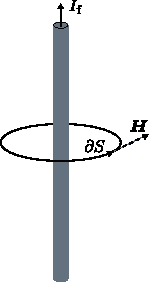
\includegraphics[height=0.7\textheight]{fig/lec07/Magnetic_field_strength_simple_conductor.pdf}
				\caption{Illustration of the magnetic field strength $\bm{H}$ around a simple conductor}
			\end{figure}
		\end{column}
		\end{columns}
\end{frame}


%%%%%%%%%%%%%%%%%%%%%%%%%%%%%%%%%%%%%%%%%%%%%%%%%%%%%%%%%%%%%
%% Ampere's circuital law: free current example %%
%%%%%%%%%%%%%%%%%%%%%%%%%%%%%%%%%%%%%%%%%%%%%%%%%%%%%%%%%%%%%
\begin{frame}
	\frametitle{Amp\`ere's circuital law: free current example}
	\begin{columns}
		\begin{column}{0.55\textwidth}
			What is the free current $I_{\mathrm{f}}$ enclosed by the loop $\partial S$?
            \begin{itemize}
                \item<2-> The current $I_1$ flows in the direction of the loop $\partial S$ (according to right-hand rule).
                \item<3-> The current $I_1$ must be counted $N$ times due to the $N$ turns of wire around the loop $\partial S$.
                \item<4-> The current $I_2$ flows in the opposite direction of the loop $\partial S$ (according to right-hand rule).
                \item<5-> Result:
            \end{itemize}
            \vspace{0.25cm}
            \onslide<5->{\begin{equation*}
                I_\mathrm{f} = N \cdot I_1 - I_2.
            \end{equation*}}
		\end{column}
        \hfill
		\begin{column}{0.45\textwidth}
			\begin{figure}
				\centering
				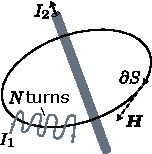
\includegraphics[height=0.5\textheight]{fig/lec07/Magnetic_field_strength_multiple_conductors.pdf}
				\caption{Arrangement with two electrical conductors}
			\end{figure}
		\end{column}
		\end{columns}
\end{frame}

%%%%%%%%%%%%%%%%%%%%%%%%%%%%%%%%%%%%%%%%%%%%%%%%%%%%%%%%%%%%%
%% Ampere's circuital law: simple solenoid  example%%
%%%%%%%%%%%%%%%%%%%%%%%%%%%%%%%%%%%%%%%%%%%%%%%%%%%%%%%%%%%%%
\begin{frame}
	\frametitle{Amp\`ere's circuital law: simple solenoid example}
	\begin{columns}
		\begin{column}{0.575\textwidth}
			Ampere's law for magnetic flux density $\bm{B}$ in vacuum:
            \begin{align}
                \mbox{Integral form:} \quad &\oint_{\partial S} \bm{B} \cdot \mathrm{d}\bm{s} = \mu_0 I,\\
                \mbox{Differential form:} \quad &\nabla \times \bm{B} = \mu_0\bm{J}. 
            \end{align}
            Here, $\mu_0$ is the permeability of free space, $\bm{J}$ is the total current density and $I$ is the total current enclosed by the loop $\partial S$. 
            \vspace{0.25cm}
            \begin{itemize}
                \item<2-> SI-unit: $[B] = \si{\tesla} = \si{\volt\second\per\metre\squared} = \si{\newton\per\ampere\per\metre}$
                \item<3-> Example contour $\partial S$  on the right covering $N$ turns and length $l$ (flux density within solenoid):
            \end{itemize}
            \onslide<4->{$$\oint_{\partial S} \bm{B} \cdot \mathrm{d}\bm{s} = N \mu_0 I  \Leftrightarrow B = \frac{N \mu_0 I}{l}$$}
		\end{column}
        \hfill
		\begin{column}{0.425\textwidth}
            \vspace{-0.2cm}
			\begin{figure}
				\centering
				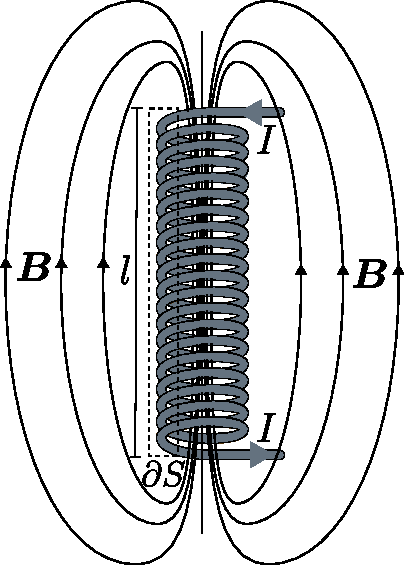
\includegraphics[height=0.68\textheight]{fig/lec07/Solenoid_Ampere_law.pdf}
				\caption{Magnetic flux density evaluated at the contour $\partial \bm{S}$  (adapted from: \href{https://commons.wikimedia.org/wiki/File:Solenoid_and_Ampere_Law.png}{Wikimedia Commons}, Goodphy, \href{https://creativecommons.org/licenses/by-sa/4.0/deed.en}{CC BY-SA 4.0})}
			\end{figure}
		\end{column}
		\end{columns}
\end{frame}

%%%%%%%%%%%%%%%%%%%%%%%%%%%%%%%%%%%%%%%%%%%%%%%%%%%%%%%%%%%%%
%% Shortcomings of the Ampere's circuital law %%
%%%%%%%%%%%%%%%%%%%%%%%%%%%%%%%%%%%%%%%%%%%%%%%%%%%%%%%%%%%%%
\begin{frame}
	\frametitle{Shortcomings of the Amp\`ere's circuital law}
	\begin{columns}
		\begin{column}{0.55\textwidth}
			Applying Amp\`ere's circuital law to a capacitor with a changing electric field $\bm{E}$ leads to a contradiction:
            \begin{itemize}
                \item Applying \eqref{eq:ampere_law} to $S_1$ yields:
                $$\oint_{\partial S_1} \bm{H} \cdot \mathrm{d}\bm{s} = I.$$
                \item<2-> In the case of $S_2$ we receive:
                $$\oint_{\partial S_2} \bm{H} \cdot \mathrm{d}\bm{s} = 0.$$
                \item<3-> However, both surfaces share the same bounding contour $\partial S$.
                \item<4-> Issue: The magnetic field strength $\bm{H}$ is not able to describe the displacement current.
            \end{itemize}
		\end{column}
        \hfill
		\begin{column}{0.45\textwidth}
			\begin{figure}
				\centering
				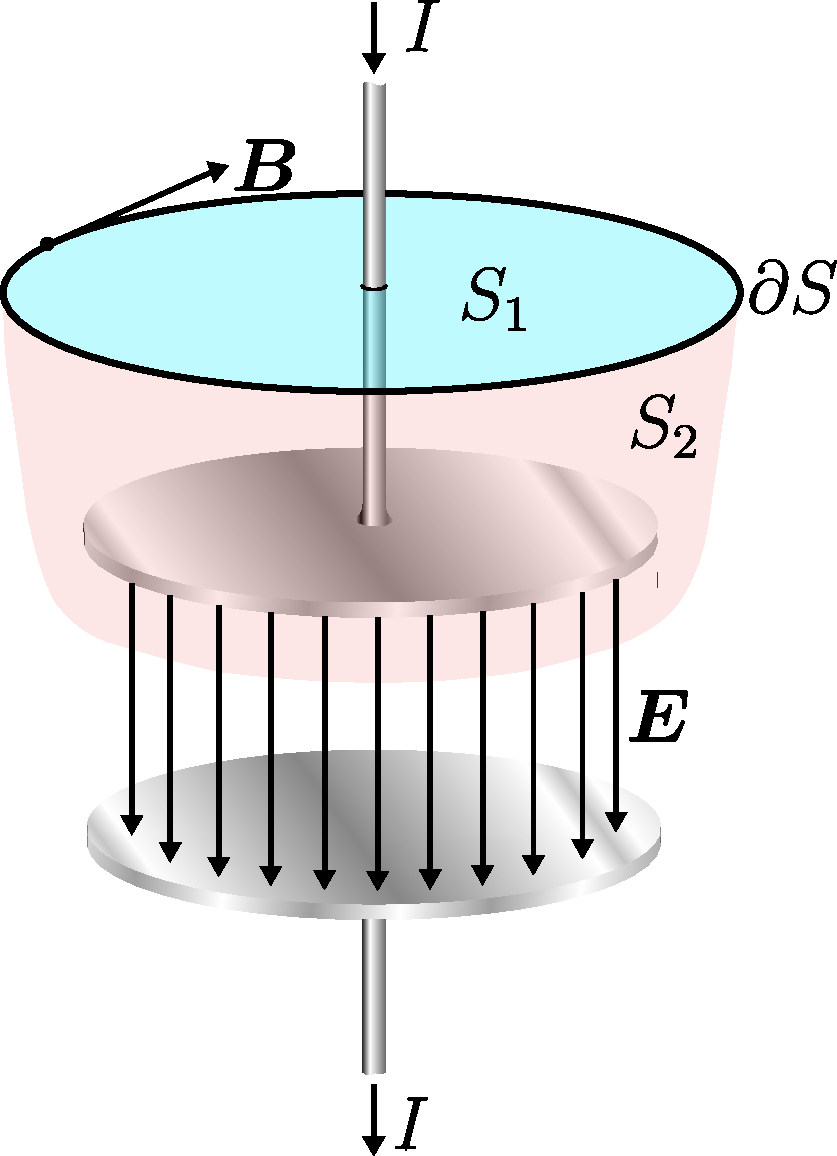
\includegraphics[height=0.55\textheight]{fig/lec07/Displacement_current_in_capacitor.pdf}
				\caption{Surfaces $S_1$ and $S_2$ share the same bounding contour $\partial S$. However, $S_1$ is pierced by conduction current, while $S_2$ is pierced by displacement current (adapted from: \href{https://commons.wikimedia.org/wiki/File:Displacement_current_in_capacitor.svg}{Wikimedia Commons}, public domain).}
			\end{figure}
		\end{column}
		\end{columns}
\end{frame}

%%%%%%%%%%%%%%%%%%%%%%%%%%%%%%%%%%%%%%%%%%%%%%%%%%%%%%%%%%%%%
%% Lorentz force %%
%%%%%%%%%%%%%%%%%%%%%%%%%%%%%%%%%%%%%%%%%%%%%%%%%%%%%%%%%%%%%
\begin{frame}
	\frametitle{Lorentz force}
    \begin{columns}
		\begin{column}{0.6\textwidth}
        The force $\bm{F}$ acting on a particle of electric charge $q$ with instantaneous velocity $\bm{v}$, due to an external electric field $\bm{E}$ and magnetic field $\bm{B}$, is given by
            \begin{equation}
                \bm{F} = q\left(\bm{E} + \bm{v}\times\bm{B}\right).
            \end{equation}
            \pause
            \begin{itemize}
                \item The term $q\bm{E}$  is called the electric force. \pause
                \item The term $q\left(\bm{v}\times\bm{B}\right)$ is called the magnetic force. \pause
                \item In Cartesian coordinates, the Lorentz force is given by:
            \end{itemize}
            \begin{equation}
                \begin{aligned}
                    F_x &= q\left(E_x + v_yB_z - v_zB_y\right),\\
                    F_y &= q\left(E_y + v_zB_x - v_xB_z\right),\\
                    F_z &= q\left(E_z + v_xB_y - v_yB_x\right).
                \end{aligned}
            \end{equation}
		\end{column}
        \hfill
		\begin{column}{0.40\textwidth}
			\begin{figure}
				\centering
				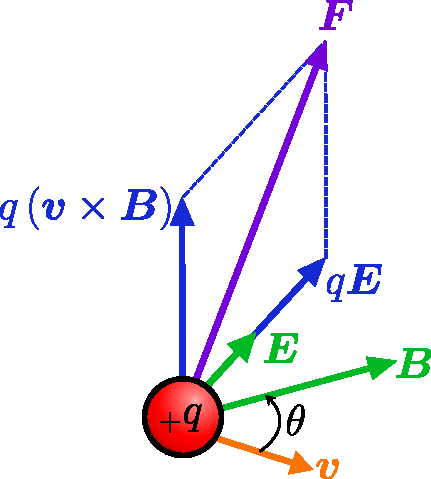
\includegraphics[height=0.5\textheight]{fig/lec07/Lorentz_force_particle.pdf}
				\caption{Lorentz force $\bm{F}$ on a particle (of charge $q$) in motion (instantaneous velocity $\bm{v}$) with given $\bm{E}$ and $\bm{B}$ fields (adapted from: \href{https://commons.wikimedia.org/wiki/File:Lorentz_force_particle.svg}{Wikimedia Commons}, Maschen, \href{https://creativecommons.org/publicdomain/zero/1.0/deed.en}{CC0})}
			\end{figure}
		\end{column}
		\end{columns}
\end{frame}

%%%%%%%%%%%%%%%%%%%%%%%%%%%%%%%%%%%%%%%%%%%%%%%%%%%%%%%%%%%%%
%% Hand rule of the magnetic Lorentz force %%
%%%%%%%%%%%%%%%%%%%%%%%%%%%%%%%%%%%%%%%%%%%%%%%%%%%%%%%%%%%%%
\begin{frame}
	\frametitle{Hand rule of the magnetic Lorentz force}
    \begin{figure}
        \centering
        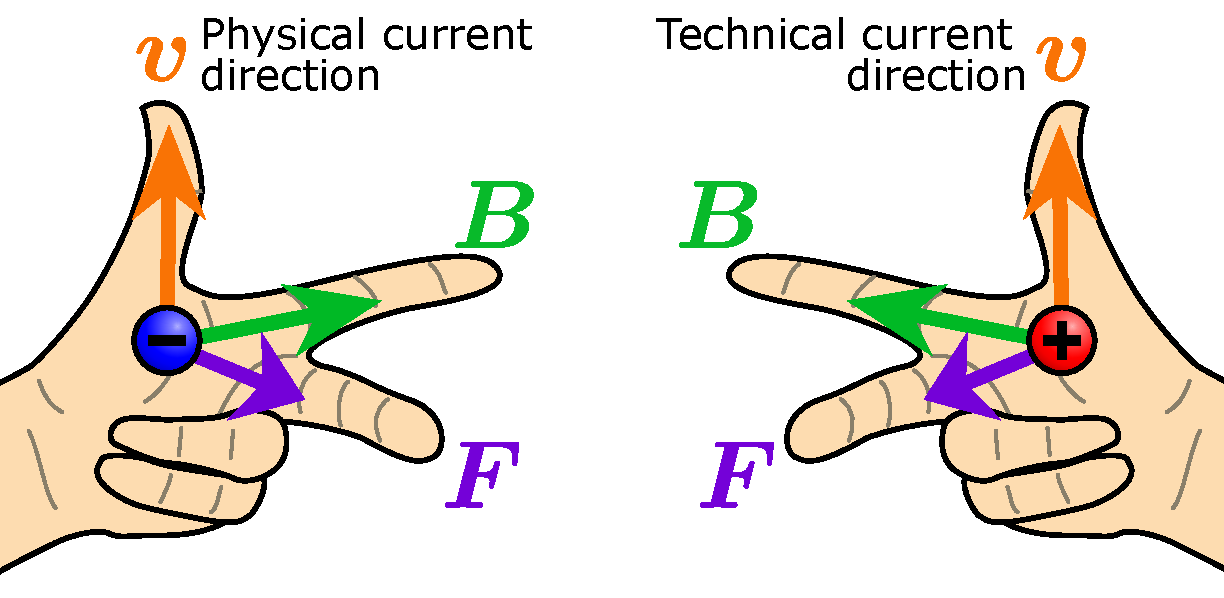
\includegraphics[height=0.6\textheight]{fig/lec07/Hand-rule-charges-both-hands.pdf}
        \caption{Right and left hand rule for the magnetic Lorentz force $q\left(\bm{v}\times\bm{B}\right)$ (adapted from: \href{https://commons.wikimedia.org/wiki/File:Right-hand-rule-charges-both-hands.svg}{Wikimedia Commons}, M. Run, \href{https://creativecommons.org/licenses/by-sa/3.0/deed.en}{CC BY-SA 3.0})}
    \end{figure}
\end{frame}

%%%%%%%%%%%%%%%%%%%%%%%%%%%%%%%%%%%%%%%%%%%%%%%%%%%%%%%%%%%%%
%% Lorentz force density for a continuous charge distribution %%
%%%%%%%%%%%%%%%%%%%%%%%%%%%%%%%%%%%%%%%%%%%%%%%%%%%%%%%%%%%%%
\begin{frame}
	\frametitle{Lorentz force density for a continuous charge distribution}
    \begin{columns}
		\begin{column}{0.5\textwidth}
         For a continuous charge distribution in motion, the Lorentz force density (force per unit volume) becomes: 
            \begin{equation}
                \bm{f} = \rho\bm{E} + \bm{J}\times\bm{B}.
            \end{equation}
            \begin{itemize}
                \item $\rho$ is the charge density (charge per unit volume).
                \item $\bm{J} = \rho \bm{v}$ is the current density.
            \end{itemize}
		\end{column}
        \hfill
		\begin{column}{0.5\textwidth}
			\begin{figure}
				\centering
				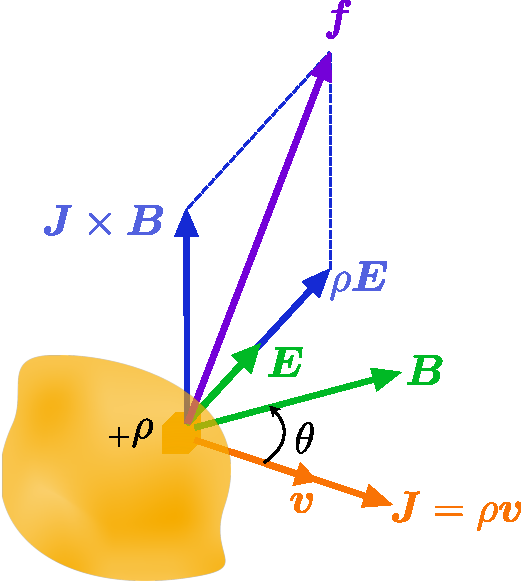
\includegraphics[height=0.6\textheight]{fig/lec07/Lorentz_force_continuum.pdf}
				\caption{Lorentz force density $\bm{f}$ on a continuous charge distribution (charge density $\rho$) in motion (adapted from: \href{https://commons.wikimedia.org/wiki/File:Lorentz_force_continuum.svg}{Wikimedia Commons}, Maschen, \href{https://creativecommons.org/publicdomain/zero/1.0/deed.en}{CC0})}
			\end{figure}
		\end{column}
		\end{columns}
\end{frame}

%%%%%%%%%%%%%%%%%%%%%%%%%%%%%%%%%%%%%%%%%%%%%%%%%%%%%%%%%%%%%
%% The Ampere--Maxwell equation %%
%%%%%%%%%%%%%%%%%%%%%%%%%%%%%%%%%%%%%%%%%%%%%%%%%%%%%%%%%%%%%
\begin{frame}
	\frametitle{The Amp\`ere -- Maxwell equation}
	\begin{columns}
		\begin{column}{0.6\textwidth}
			The charge of capacitor is:
            $$Q = \oint_{S_2} \bm{D}\cdot \mathrm{d}\bm{S}.$$
            \onslide<2->{If the electric field ($\bm{D} = \varepsilon_0\varepsilon_\mathrm{r} \bm{E}$) changes, a displacement current results:
            $$I_{\mathrm{d}} = \frac{\mathrm{d}}{\mathrm{d} t} \oint_{S_2} \bm{D}\cdot \mathrm{d}\bm{S}$$}
            \begin{itemize}
                \item<3-> Is not a classical electric current (moving charges) but a term to describe the changing electric field.
                \item<4-> Above, $\varepsilon_0$ is the vacuum permittivity and $\varepsilon_\mathrm{r}$ is the relative permittivity of a material.
            \end{itemize}
		\end{column}
        \hfill
		\begin{column}{0.4\textwidth}
			\begin{figure}
				\centering
				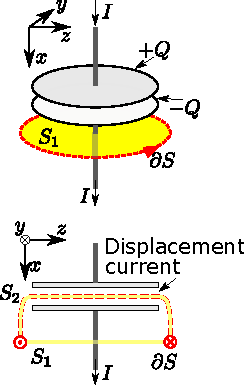
\includegraphics[height=0.65\textheight]{fig/lec07/Maxwell_integral_displacement_current.pdf}
				\caption{Illustration for calculating the displacement current (adapted from: \href{https://commons.wikimedia.org/wiki/File:Maxwell_integral_displacement_current.svg}{Wikimedia Commons}, public domain).}
			\end{figure}
		\end{column}
		\end{columns}
\end{frame}

%%%%%%%%%%%%%%%%%%%%%%%%%%%%%%%%%%%%%%%%%%%%%%%%%%%%%%%%%%%%%
%% The Ampere--Maxwell equation (cont.)%%
%%%%%%%%%%%%%%%%%%%%%%%%%%%%%%%%%%%%%%%%%%%%%%%%%%%%%%%%%%%%%
\begin{frame}
	\frametitle{The Amp\`ere -- Maxwell equation (cont.)}
        Adding the displacement current to \eqref{eq:ampere_law} we receive the Amp\`ere -- Maxwell equation:
            \begin{align}    
            \mbox{Integral form:} \quad  &\int_{\partial S} \bm{H} \cdot \mathrm{d}\bm{s} = \iint_{S}\left(\bm{J}_\mathrm{f} + \frac{\mathrm{d}}{\mathrm{d} t} \bm{D} \right)\cdot\mathrm{d}\bm{S}, \\
            \mbox{Differential form:} \quad &\nabla \times \bm{H} = \bm{J}_\mathrm{f} +  \frac{\partial\bm{D}}{\partial t}. 
            \label{eq:ampere_maxwell_law}
        \end{align}
        Above, $\bm{D}$ is the electric displacement field.
        \vspace{0.5cm}
        \begin{itemize}
            \item SI-unit: $[D] = \si{\coulomb\per\metre\squared}$
            \item SI-unit: $[E] = \si{\volt\per\metre}$
            \item $\varepsilon_0 \approx \SI{8.854e-12}{\farad\per\metre}$
        \end{itemize}
\end{frame}

%%%%%%%%%%%%%%%%%%%%%%%%%%%%%%%%%%%%%%%%%%%%%%%%%%%%%%%%%%%%%
%% Ampere's circuital law: magnetic flux %%
%%%%%%%%%%%%%%%%%%%%%%%%%%%%%%%%%%%%%%%%%%%%%%%%%%%%%%%%%%%%%
\begin{frame}
	\frametitle{Magnetic flux and flux linkage}
	\begin{columns}
		\begin{column}{0.575\textwidth}
			The magnetic flux $\phi$ is the surface integral of the normal component of $\bm{B}$ over that surface:
            \begin{align}
                \phi = \iint_{S} \bm{B} \cdot \mathrm{d}\bm{S}. 
            \end{align}
            \onslide<2->{As there are no magnetic monopoles, the magnetic flux through a closed surface (which is covering a volume without holes) is always zero:
            \begin{align}
                \oint_{S} \bm{B} \cdot \mathrm{d}\bm{S} = 0.
            \end{align}}
            \onslide<3->{The flux linkage $\psi$ is the product of the magnetic flux $\phi$ and the number of turns $N$ of a coil:
            \begin{align}
                \psi = N  \phi.
            \end{align}}
		\end{column}
        \hfill
		\begin{column}{0.425\textwidth}
            \vspace{-0.4cm}
			\begin{figure}
				\centering
				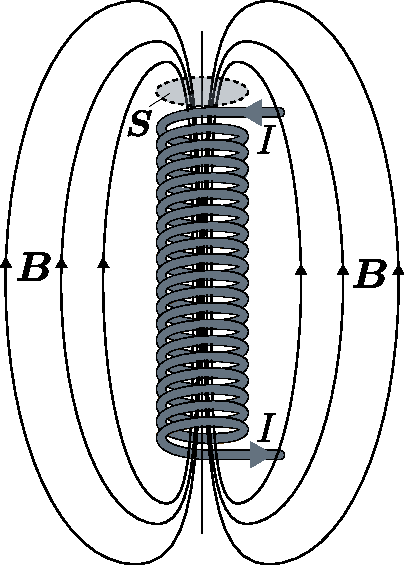
\includegraphics[height=0.68\textheight]{fig/lec07/Solenoid_Flux.pdf}
				\caption{Magnetic flux $\phi$ evaluated at the surface $\bm{S}$  (adapted from: \href{https://commons.wikimedia.org/wiki/File:Solenoid_and_Ampere_Law.png}{Wikimedia Commons}, Goodphy, \href{https://creativecommons.org/licenses/by-sa/4.0/deed.en}{CC BY-SA 4.0})}
                \label{fig:Solenoid_Flux}
			\end{figure}
		\end{column}
		\end{columns}
\end{frame}

%%%%%%%%%%%%%%%%%%%%%%%%%%%%%%%%%%%%%%%%%%%%%%%%%%%%%%%%%%%%%
%% Magnetic leakage flux %%
%%%%%%%%%%%%%%%%%%%%%%%%%%%%%%%%%%%%%%%%%%%%%%%%%%%%%%%%%%%%%
\begin{frame}
	\frametitle{Magnetic leakage flux}
	\begin{columns}
		\begin{column}{0.48\textwidth}
			\begin{itemize}
                \item In the scenarios with multiple coils, the magnetic flux generated by one coil will influence also the other coils.
                \item Exception: two coils are perfectly perpendicular to each other.
                \item However, the magnetic flux typically does not fully couple with the other coils
                \item The difference is the leakage flux $\phi_\sigma$.
            \end{itemize}
		\end{column}
        \hfill
		\begin{column}{0.48\textwidth}
            \vspace{-0.2cm}
			\begin{figure}
				\centering
				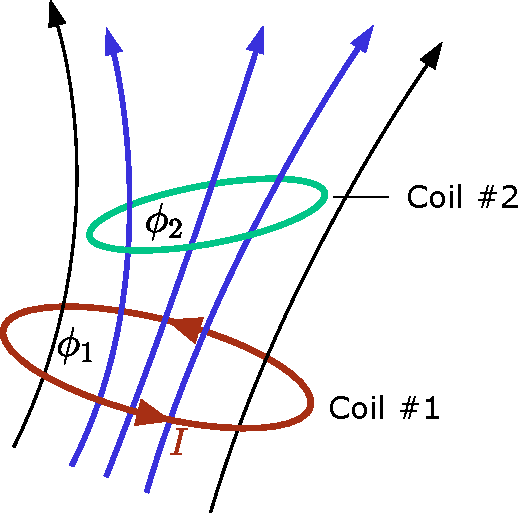
\includegraphics[height=0.55\textheight]{fig/lec07/Leakage_flux.pdf}
				\caption{The magnetic flux $\phi_1$ generated by the current $I$ does only partly couple with the second coil, while the difference $\phi_1-\phi_2$ is the leakage flux (adapted from: \href{https://commons.wikimedia.org/wiki/File:Mutual_Inductivity.svg}{Wikimedia Commons}, M. Wacenovsky, public domain)}
			\end{figure}
		\end{column}
		\end{columns}
\end{frame}


%%%%%%%%%%%%%%%%%%%%%%%%%%%%%%%%%%%%%%%%%%%%%%%%%%%%%%%%%%%%%
%% Leakage flux
%%%%%%%%%%%%%%%%%%%%%%%%%%%%%%%%%%%%%%%%%%%%%%%%%%%%%%%%%%%%%
\begin{frame}
    \frametitle{Magnetic leakage flux}
    \begin{columns}
        \begin{column}{0.58\textwidth}
            Not all magnetic flux generated by one winding links the other winding.
            \vspace{0.15cm}
            The uncoupled portion of flux is called leakage flux.
            \vspace{0.15cm}
            Leakage flux:
            \begin{itemize}
                \item Does not contribute to energy transfer.
                \item Produces voltage overshoot.
                \item Creates ringing during switching transitions.
                \item Becomes important at high switching frequencies.
            \end{itemize}
            \vspace{0.15cm}
            Leakage flux is inevitable in practical transformers.
        \end{column}
        \begin{column}{0.38\textwidth}
            \begin{figure}
                \centering
                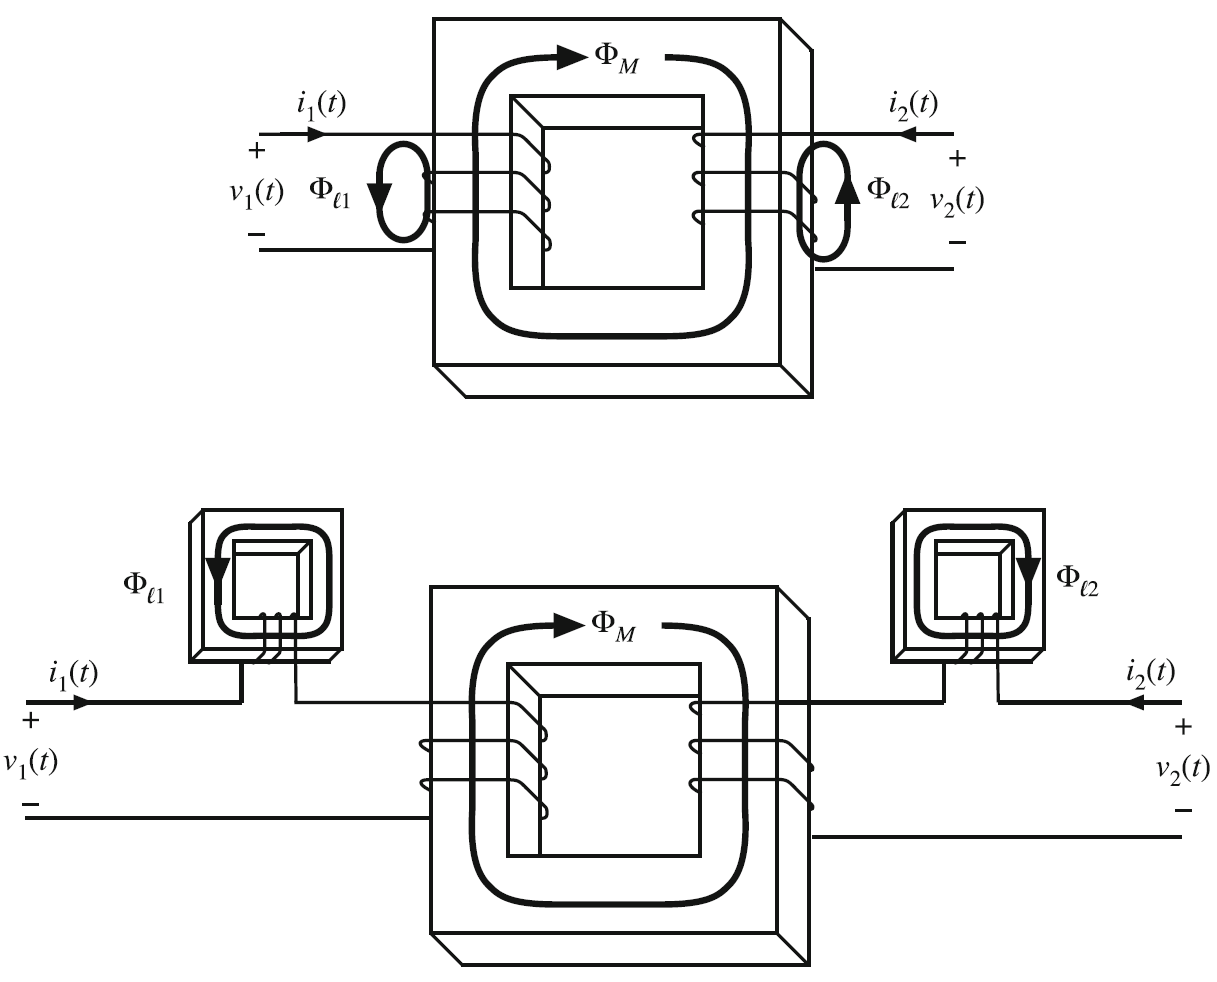
\includegraphics[width=\linewidth]{fig/lec07/Leakage_Flux.png}
                \caption{Leakage-flux paths that do not couple both windings. Adapted from Erickson and Maksimovic, \textit{Fundamentals of Power Electronics}, 3rd edition, Springer, 2013.}
            \end{figure}
        \end{column}
    \end{columns}
\end{frame}


%%%%%%%%%%%%%%%%%%%%%%%%%%%%%%%%%%%%%%%%%%%%%%%%%%%%%%%%%%%%% %% Lenz's law %%%%%%%%%%%%%%%%%%%%%%%%%%%%%%%%%%%%%%%%%%%%%%%%%%%%%%%%%%%%%
\begin{frame} 
    \frametitle{Lenz's Law: Direction of Induced Voltage and Current} 
    \begin{columns} 
        \begin{column}{0.58\textwidth} 
            Lenz's law defines the polarity of the induced voltage. The induced current always acts in a direction that opposes the change in magnetic flux that produced it. 
            \vspace{0.2cm} 
            \begin{itemize} 
                \item If the original flux increases, the induced current produces an opposing flux. 
                \item If the original flux decreases, the induced current tries to maintain it. 
                \item This is a direct consequence of energy conservation. 
                \item Lenz's law explains eddy currents, transformer action, leakage effects, and magnetic damping. 
            \end{itemize} 
            \vspace{0.2cm} 
            For a shorted conducting loop, 
            \begin{align} v_{\mathrm{ind}}(t)=\frac{d\Phi(t)}{dt}, \qquad i_{\mathrm{ind}}(t)=\frac{v_{\mathrm{ind}}(t)}{Z_{\mathrm{loop}}} 
            \end{align} The induced current produces a secondary flux that opposes the original flux variation. 
        \end{column} 
        \begin{column}{0.38\textwidth} 
            \begin{figure} 
                \centering 
                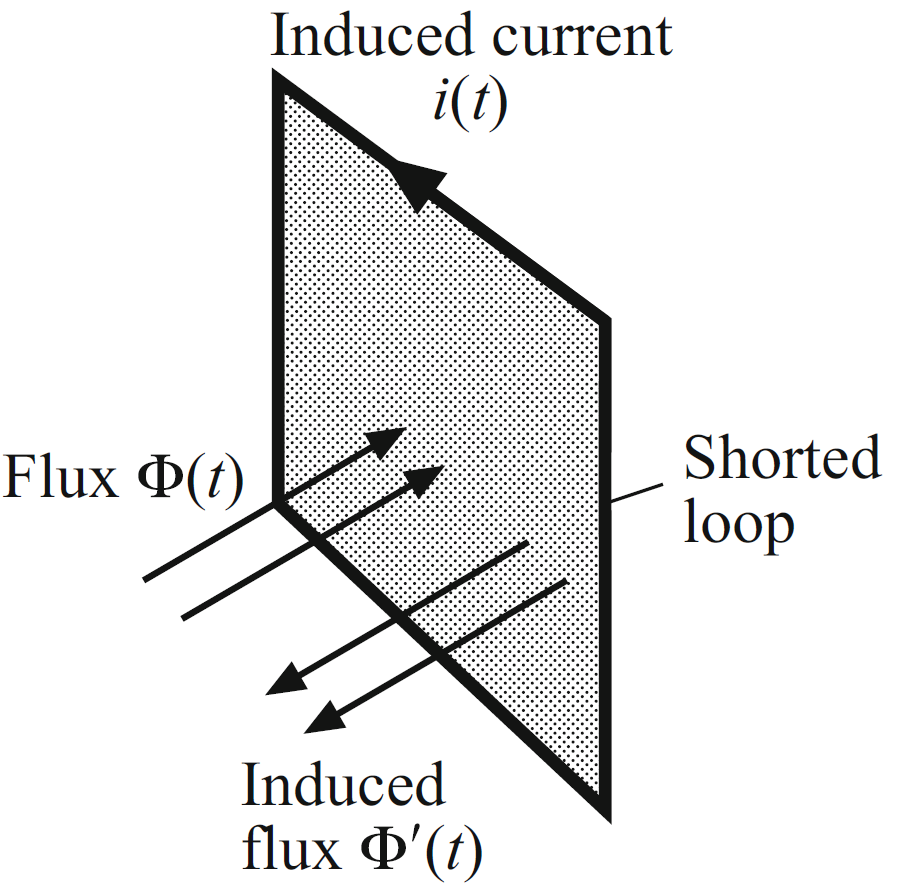
\includegraphics[width=0.75\linewidth]{fig/lec07/Lenz_law.png} 
                \caption{Lenz's law in a shorted loop: the induced current produces flux opposing the applied flux variation. Adapted from Erickson and Maksimovic, \textit{Fundamentals of Power Electronics}, 3rd edition, Springer, 2013.}
            \end{figure} 
        \end{column} 
    \end{columns} 
\end{frame}




%%%%%%%%%%%%%%%%%%%%%%%%%%%%%%%%%%%%%%%%%%%%%%%%%%%%%%%%%%%%%
%% Inductance %%
%%%%%%%%%%%%%%%%%%%%%%%%%%%%%%%%%%%%%%%%%%%%%%%%%%%%%%%%%%%%%
\begin{frame}
	\frametitle{Inductance}
	The inductance $L$ describes the ratio between the magnetic flux linkage $\psi(t)$ to the current $i(t)$:
    \begin{align}
        \psi(t) = L i(t).
    \end{align}
    \pause
    \textbf{Example}:  From the solenoid in \figref{fig:Solenoid_Flux} we know that the magnetic flux linkage $\psi$ is:
    $$\psi = N \iint_{S} \bm{B} \cdot \mathrm{d}\bm{S}= \frac{1}{l}N^2 \mu_0 I \pi r^2 $$
    with $r$ being the radius of the solenoid. \pause Hence, the inductance $L$ is:
    $$L = \frac{\psi}{I} = \frac{N^2 \mu_0 \pi r^2}{l}.$$
    \begin{itemize}
        \item SI-unit: $[L] = \si{\henry} = \si{\volt\second\per\ampere}$
        \item The inductance is an important parameter describing inductive systems.
    \end{itemize}
\end{frame}

%%%%%%%%%%%%%%%%%%%%%%%%%%%%%%%%%%%%%%%%%%%%%%%%%%%%%%%%%%%%%
%% Self and mutual inductance %%
%%%%%%%%%%%%%%%%%%%%%%%%%%%%%%%%%%%%%%%%%%%%%%%%%%%%%%%%%%%%%
\begin{frame}
	\frametitle{Self and mutual inductance}
    \begin{columns}
		\begin{column}{0.45\textwidth}
            Based on the inductive coupling between the two coils from \figref{fig:Transformer3d_col3}, we can define the magnetic flux matrix:
            \begin{equation}
                \bm{\phi} = \begin{bmatrix} \phi_{11} & \phi_{12} \\ \phi_{21} & \phi_{22} \end{bmatrix} .
                \label{eq:flux_matrix_transformer}
            \end{equation}
            \vspace{-0.2cm}
			\begin{itemize}
                \item<2-> $\phi_{11}$: magnetic flux component of coil 1 due to its own current $i_1$
                \item<3-> $\phi_{12}$: magnetic flux component of coil 1 due to the current $i_2$ in coil 2
                \item<4-> $\phi_{21}$: magnetic flux component of coil 2 due to the current $i_1$ in coil 1
                \item<5-> $\phi_{22}$: magnetic flux component of coil 2 due to its own current $i_2$
            \end{itemize}
		\end{column}
        \hfill
		\begin{column}{0.525\textwidth}
			\begin{figure}
				\centering
				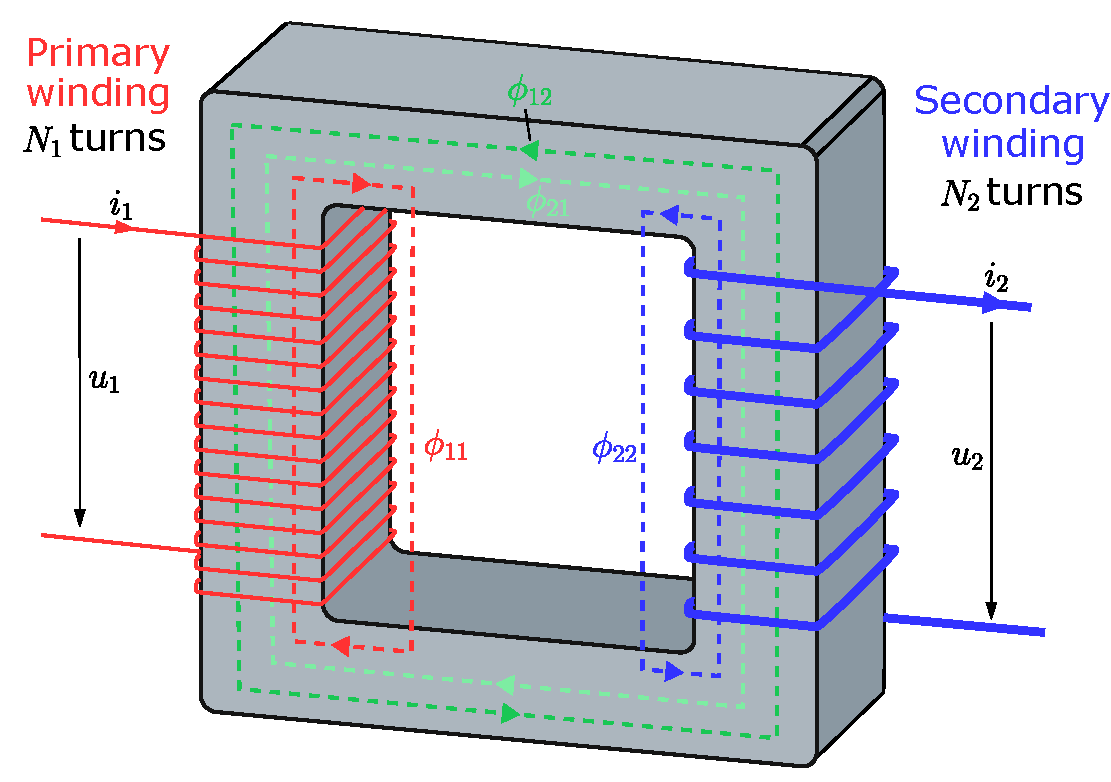
\includegraphics[height=0.575\textheight]{fig/lec07/Transformer3d_col3.pdf}
				\caption{Two coils coupled via a common core (adapted from: \href{https://commons.wikimedia.org/wiki/File:Transformer3d_col3.svg}{Wikimedia Commons}, Bill C., \href{https://creativecommons.org/licenses/by-sa/3.0/deed.en}{CC~BY-SA~3.0})}
                \label{fig:Transformer3d_col3}
			\end{figure}
		\end{column}
		\end{columns}
\end{frame}

%%%%%%%%%%%%%%%%%%%%%%%%%%%%%%%%%%%%%%%%%%%%%%%%%%%%%%%%%%%%%
%% Self and mutual inductance (cont.) %%
%%%%%%%%%%%%%%%%%%%%%%%%%%%%%%%%%%%%%%%%%%%%%%%%%%%%%%%%%%%%%
\begin{frame}
	\frametitle{Self and mutual inductance (cont.)}
    Utilizing the permeance definition (``magnetic conductance'') 
    \begin{equation}
        \Lambda = \frac{\phi}{N i},
    \end{equation}
    \pause
    we can represent \eqref{eq:flux_matrix_transformer} as:
    \begin{equation}
        \phi_{11} = \Lambda_{11} N_1 i_1, \quad \phi_{12} = \Lambda_{12} N_2 i_2, \quad \phi_{21} = \Lambda_{21} N_1 i_1, \quad \phi_{22} = \Lambda_{22} N_2 i_2.
    \end{equation}
    \pause
    The resulting flux linkage per coil is then:
    \begin{equation}
        \begin{alignedat}{3}
        \psi_1 &= N_1\left(\phi_{11} + \phi_{21} + \phi_{12}\right), \quad && \psi_2 && =  N_2\left(\phi_{22} + \phi_{12} + \phi_{21}\right),\\ \pause
               &=\underbrace{\left(\Lambda_{11}N_1^2+\Lambda_{21}N_1^2\right)}_{L_1}i_1 + \underbrace{\Lambda_{12}N_1N_2}_{M_{12}}i_2, \quad && && =\underbrace{\left(\Lambda_{22}N_2^2+\Lambda_{12}N_1^2\right)}_{L_2}i_2 + \underbrace{\Lambda_{21}N_1N_2}_{M_{21}}i_1. 
        \end{alignedat}
        \label{eq:flux_linkage_transformer}
    \end{equation}
    Above, $L_1$ and $L_2$ are the self-inductances, $M_{12}$ and $M_{21}$ are the mutual inductances.
\end{frame}

%%%%%%%%%%%%%%%%%%%%%%%%%%%%%%%%%%%%%%%%%%%%%%%%%%%%%%%%%%%%%
%% Self and mutual inductance (cont.) %%
%%%%%%%%%%%%%%%%%%%%%%%%%%%%%%%%%%%%%%%%%%%%%%%%%%%%%%%%%%%%%
\begin{frame}
	\frametitle{Self and mutual inductance (cont.)}
    Hence, we can define the flux linkages of both coils using the following inductance matrix:
    \begin{equation}
        \bm{\psi} = \begin{bmatrix} \psi_1 \\ \psi_2 \end{bmatrix} = \begin{bmatrix} L_1 & M_{12} \\ M_{21} & L_2 \end{bmatrix} \begin{bmatrix} i_1 \\ i_2 \end{bmatrix} = \bm{L}\bm{i}.
        \label{eq:flux_linkage_matrix_transformer}
    \end{equation}
    \pause
    Due to the symmetry of the inductive coupling, the mutual inductances are identical:
    \begin{equation}
        M_{12} = M_{21} = M.
    \end{equation}
    \pause
    Based on \eqref{eq:flux_linkage_transformer}, we can also split the self-inductance $L_i$ of the $i$-th coil into the sum of the leakage inductance $L_{i,\sigma}$ and the magnetizing inductance $L_{i,\mathrm{m}}$:
    \begin{equation}
        L_i = L_{i,\sigma} + L_{i,\mathrm{m}} = \Lambda_{ii}N_i^2 + \Lambda_{ji}N_i^2 \quad \mbox{with} \quad i \neq j. 
        \label{eq:inductance_split}
    \end{equation}
    \pause
    Finally, we can define the coupling coefficient $k$ as:
    \begin{equation}
        k = \frac{M}{\sqrt{L_1 L_2}}, \qquad 0 \leq k \leq 1,
        \label{eq:coupling_coefficient}
    \end{equation}
    which indicates how strong or week the inductive coupling between the coils is.
\end{frame}


%%%%%%%%%%%%%%%%%%%%%%%%%%%%%%%%%%%%%%%%%%%%%%%%%%%%%%%%%%%%%
%% Leakage inductance
%%%%%%%%%%%%%%%%%%%%%%%%%%%%%%%%%%%%%%%%%%%%%%%%%%%%%%%%%%%%%
\begin{frame}
    \frametitle{Leakage Inductance}
    \begin{columns}
        \begin{column}{0.58\textwidth}
            The energy associated with leakage flux is represented electrically as leakage inductance.
            \vspace{0.15cm}
            Leakage inductance appears in series with the transformer windings.
            \vspace{0.15cm}
            Consequences include:
            \begin{itemize}
                \item Reduced transient response
                \item Increased switching stress
                \item Voltage spikes
                \item Resonant ringing
            \end{itemize}
            \vspace{0.15cm}
            In resonant converters, however, leakage inductance can be deliberately utilized as a functional circuit element.
        \end{column}
        \begin{column}{0.38\textwidth}
            \begin{block}{Design Objective}
                Conventional transformer:
                \begin{equation}
                    L_{lk}
                    \rightarrow
                    \mathrm{minimum}
                \end{equation}
                \vspace{0.15cm}
                LLC converter:
                \begin{equation}
                    L_{lk}
                    \rightarrow
                    \mathrm{useful}
                \end{equation}
            \end{block}
        \end{column}
    \end{columns}
\end{frame}


%%%%%%%%%%%%%%%%%%%%%%%%%%%%%%%%%%%%%%%%%%%%%%%%%%%%%%%%%%%%% %% Electrical and magnetic domains %%%%%%%%%%%%%%%%%%%%%%%%%%%%%%%%%%%%%%%%%%%%%%%%%%%%%%%%%%%%%
\begin{frame} 
\frametitle{Interaction Between Electrical and Magnetic Domains} \begin{columns} 
    \begin{column}{0.57\textwidth} 
        A magnetic component is an energy-processing interface between the electrical and magnetic domains. 
        \vspace{0.2cm} In the electrical domain, 
        \begin{align} p_e(t)=v(t)i(t) 
        \end{align} In the magnetic domain, the corresponding variables are MMF and rate of change of flux: 
        \begin{align} 
            p_m(t)=F(t)\frac{d\Phi(t)}{dt} 
        \end{align} Using Amp\`ere's and Faraday's laws, 
        \begin{align} 
            v(t)i(t) = Ni(t)\frac{d\Phi(t)}{dt} = F(t)\frac{d\Phi(t)}{dt} 
        \end{align} 
        \begin{itemize} 
            \item Voltage corresponds to flux rate. 
            \item Current corresponds to magneto-motive force. 
            \item Energy transfer occurs through magnetic field coupling. 
        \end{itemize} 
    \end{column} 
    \begin{column}{0.39\textwidth} 
        \begin{figure} 
            \centering 
            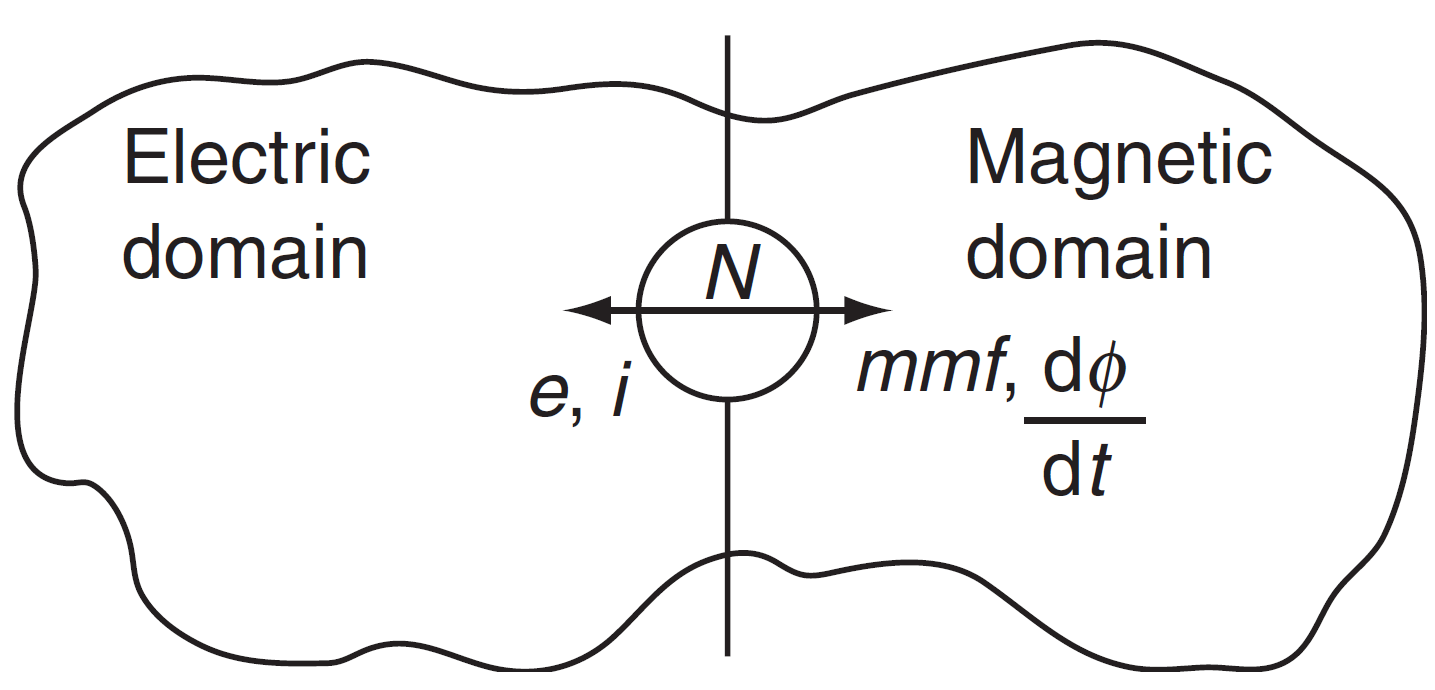
\includegraphics[width=\linewidth]{fig/lec07/electric_magnetic_domains.png} 
            \caption{Interaction between electric and magnetic domains. Adapted from Umanand, \textit{Power Electronics: Essentials and Applications}, 2nd edition, Wiley, 2012.}
        \end{figure} 
    \end{column} 
\end{columns} 
\end{frame}


%%%%%%%%%%%%%%%%%%%%%%%%%%%%%%%%%%%%%%%%%%%%%%%%%%%%%%%%%%%%% %% Electrical magnetic analogy %%%%%%%%%%%%%%%%%%%%%%%%%%%%%%%%%%%%%%%%%%%%%%%%%%%%%%%%%%%%%
\begin{frame} 
    \frametitle{Electrical--Magnetic Domain Analogy} 
    \begin{columns} 
        \begin{column}{0.56\textwidth} 
            The magnetic domain can be understood using analogies with electrical circuits. This is extremely useful for designing inductors and transformers. 
            \vspace{0.15cm} 
            \begin{table} 
                \centering 
                \small 
                \begin{tabular}{lll} 
                    \hline 
                    \textbf{Electrical} & \textbf{Magnetic} & \textbf{Meaning}\\ \hline 
                    Voltage $v$ & MMF $F$ & Driving effort\\ 
                    Current $i$ & Flux $\Phi$ & Flow quantity\\ 
                    Resistance $R$ & Reluctance $\mathcal{R}$ & Opposition to flow\\ 
                    Conductance $G$ & Permeance $\Lambda$ & Ease of flow\\ 
                    Current density $J$ & Flux density $B$ & Flow per area\\ 
                    Electric field $E$ & Magnetic field $H$ & Field intensity\\ 
                    \hline 
                \end{tabular} 
            \end{table} 
            \vspace{0.15cm} 
            The most important analogy is: 
            \begin{align} 
                V=IR \qquad \Longleftrightarrow \qquad F=\Phi\mathcal{R} 
            \end{align} 
        \end{column} 
        \begin{column}{0.40\textwidth} 
            \begin{block}{Design Interpretation} 
                \small A magnetic core behaves like a path for magnetic flux. A high-permeability core provides a low-reluctance path, just as a low-resistance conductor provides an easy path for electric current. 
            \end{block} 
            \vspace{0.2cm} 
            \begin{itemize} 
                \small 
                \item Air gaps increase reluctance. 
                \item Larger core area reduces reluctance. 
                \item Longer magnetic paths increase reluctance. 
                \item High permeability reduces reluctance. 
            \end{itemize} 
            \vspace{0.15cm}
        \end{column} 
    \end{columns} 
\end{frame}


%%%%%%%%%%%%%%%%%%%%%%%%%%%%%%%%%%%%%%%%%%%%%%%%%%%%%%%%%%%%% %% Flux and flux density %%%%%%%%%%%%%%%%%%%%%%%%%%%%%%%%%%%%%%%%%%%%%%%%%%%%%%%%%%%%%
\begin{frame} 
    \frametitle{Magnetic Flux and Flux Density} 
    \begin{columns} 
        \begin{column}{0.5\textwidth} 
            Magnetic flux $\Phi$ represents the total magnetic field passing through a given surface. Flux density $B$ represents how concentrated this flux is within the core cross-section. 
            \begin{align} 
                \Phi=\int_S \mathbf{B}\cdot d\mathbf{A} 
            \end{align} 
            For uniform flux density, 
            \begin{align} 
                \Phi=BA_c 
            \end{align} 
            \begin{align} 
            \text{Hence,} B=\frac{\Phi}{A_c} 
            \end{align} 
            where $A_c$ is the cross-sectional area of the magnetic core.
        \end{column} 
        \begin{column}{0.5\textwidth} 
            \vspace{-1.2cm}
            \begin{figure} 
                \centering 
                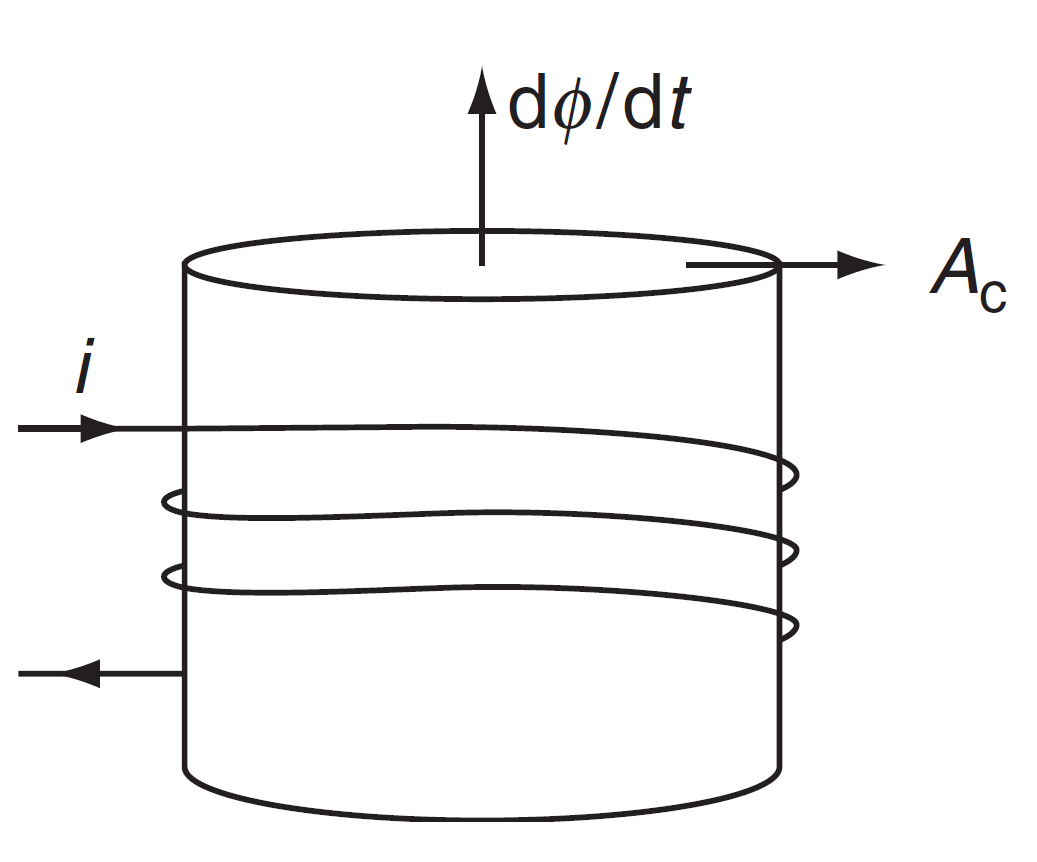
\includegraphics[width=0.5\textwidth]{fig/lec07/flux_density.png} 
                \caption{Definition of flux density in a magnetic core. Adapted from Umanand, \textit{Power Electronics: Essentials and Applications}, 2nd edition, Wiley, 2012.}
             \end{figure} 
             \vspace{-0.7cm}
            \begin{itemize} 
                \item $\Phi$ is measured in Weber. 
                \item $B$ is measured in Tesla. 
                \item $A_c$ is the effective core cross-sectional area. 
                \item A larger $A_c$ allows the same flux at lower flux density. 
                \item Excessive $B$ pushes the core toward satu. 
            \end{itemize} 
        \end{column} 
    \end{columns} 
\end{frame}



%%%%%%%%%%%%%%%%%%%%%%%%%%%%%%%%%%%%%%%%%%%%%%%%%%%%%%%%%%%%% %% H and permeability %%%%%%%%%%%%%%%%%%%%%%%%%%%%%%%%%%%%%%%%%%%%%%%%%%%%%%%%%%%%%
\begin{frame} 
    \frametitle{Magnetic Field Intensity and Permeability} 
    \begin{columns} 
        \begin{column}{0.58\textwidth} 
            The magnetic field intensity $H$ is produced by current excitation, while the flux density $B$ depends on both $H$ and the material property called permeability. 
            \begin{align} 
                B=\mu H 
            \end{align} 
            The permeability is usually written as $\mu=\mu_0\mu_r$. 
            \begin{itemize} 
                \item $\mu_0=4\pi\times10^{-7}\ \si{\henry\per\metre}$ is the permeability of free space. 
                \item $\mu_r$ is the relative permeability of the magnetic material. 
                \item Air has approximately $\mu_r=1$. 
                \item Magnetic cores may have $\mu_r$ from hundreds to many thousands. 
            \end{itemize}
        \end{column} 
        \begin{column}{0.38\textwidth} 
            \begin{figure} 
                \centering 
                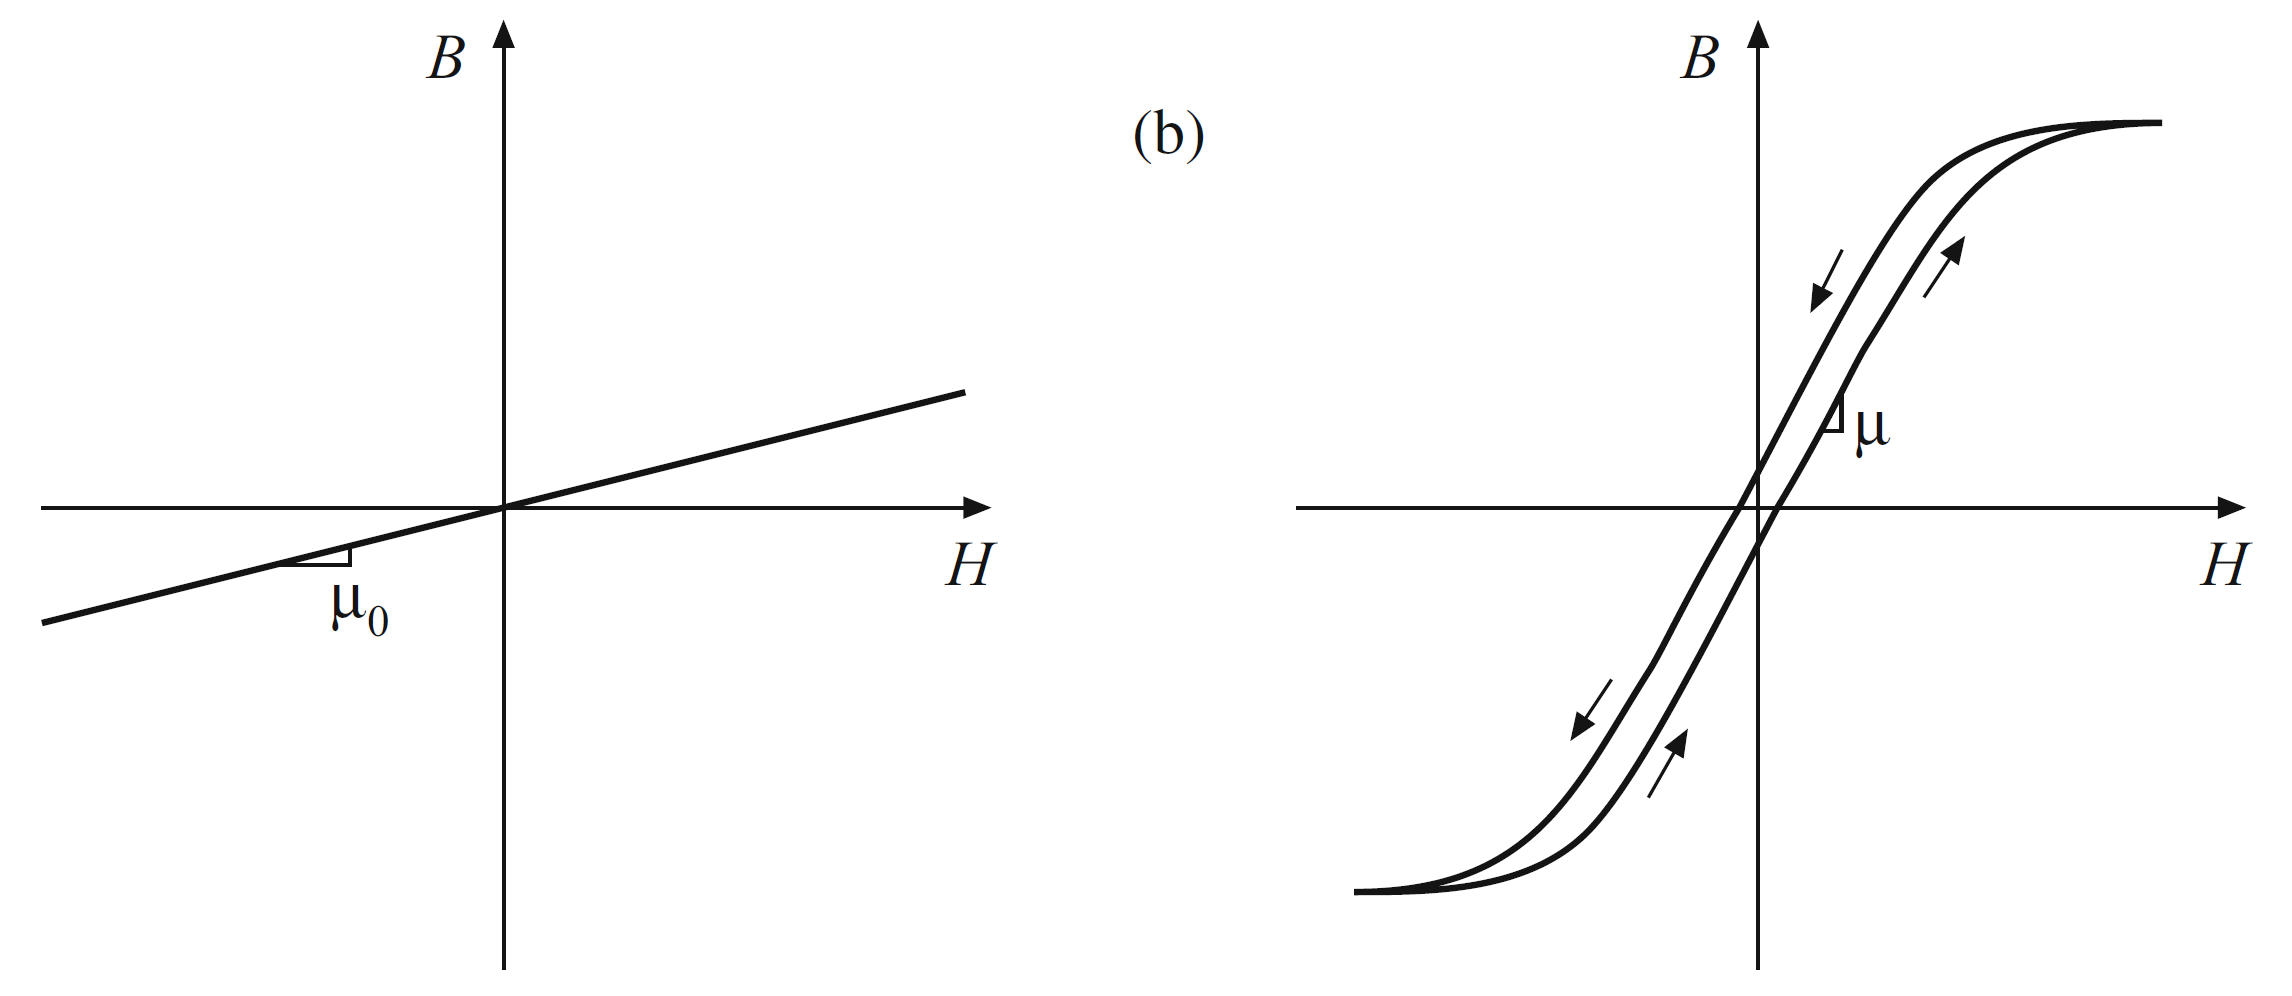
\includegraphics[width=\linewidth]{fig/lec07/air_core_material.png} 
                \caption{$B$--$H$ characteristics of air and a typical magnetic core material. Adapted from Erickson and Maksimovi\'c, Fig. 10.5.} 
            \end{figure} 
            A high value of $\mu$ means that a relatively small $H$ can produce a large $B$. 
        \end{column} 
    \end{columns} 
\end{frame}


%%%%%%%%%%%%%%%%%%%%%%%%%%%%%%%%%%%%%%%%%%%%%%%%%%%%%%%%%%%%% %% Ideal B-H curve %%%%%%%%%%%%%%%%%%%%%%%%%%%%%%%%%%%%%%%%%%%%%%%%%%%%%%%%%%%%%
\begin{frame} 
    \frametitle{Idealized $B$--$H$ Characteristic} 
    \begin{columns} 
        \begin{column}{0.57\textwidth} 
            For introductory analysis, a magnetic material is often represented using an idealized or piecewise-linear $B$--$H$ characteristic. 
            \begin{align} 
                B=\mu H 
            \end{align} 
            In the linear region, 
            \begin{itemize} 
                \item the slope of the $B$--$H$ curve is the permeability $\mu$, 
                \item flux density increases almost linearly with field intensity, 
                \item the core behaves as a predictable magnetic path, 
                \item inductance remains approximately constant. 
            \end{itemize} 
            \vspace{0.15cm} 
            However, this linear model is only valid before saturation. At high excitation, the material cannot support proportional increase in flux density. 
            \begin{align} 
                B \rightarrow B_{\mathrm{sat}} 
            \end{align} 
        \end{column} 
        \begin{column}{0.39\textwidth} 
            \begin{figure} 
                \centering 
                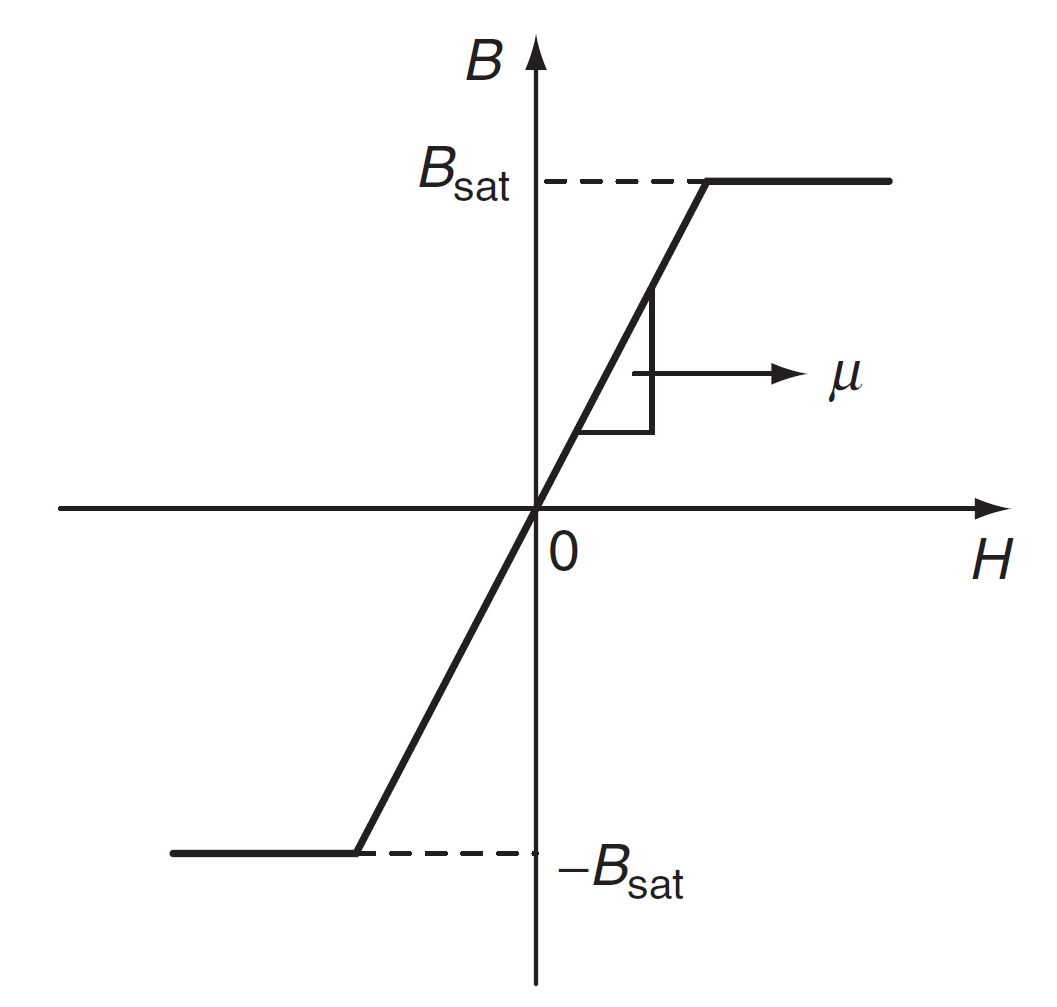
\includegraphics[width=0.8\linewidth]{fig/lec07/piecewise_linear_BH.png} 
                \caption{Piecewise-linear approximation of the $B$--$H$ curve. Adapted from Umanand, \textit{Power Electronics: Essentials and Applications}, 2nd edition, Wiley, 2012.}
            \end{figure} 
        \end{column} 
    \end{columns} 
\end{frame}


%%%%%%%%%%%%%%%%%%%%%%%%%%%%%%%%%%%%%%%%%%%%%%%%%%%%%%%%%%%%% %% Practical B-H curve and hysteresis %%%%%%%%%%%%%%%%%%%%%%%%%%%%%%%%%%%%%%%%%%%%%%%%%%%%%%%%%%%%%
\begin{frame} 
    \frametitle{Practical $B$--$H$ Characteristic and Hysteresis}
    \begin{columns} 
        \begin{column}{0.57\textwidth} 
            Practical magnetic materials do not follow a single-valued linear $B$--$H$ curve. Instead, they exhibit hysteresis: the flux density depends not only on the present value of $H$, but also on the previous magnetic history. 
            \vspace{0.15cm} 
            \begin{itemize} 
                \item During magnetization, energy is stored in the magnetic field. 
                \item During demagnetization, not all stored energy is returned. 
                \item The enclosed area of the $B$--$H$ loop represents energy lost per cycle. 
                \item This loss appears as heat in the magnetic core. 
                \item Hysteresis loss increases with switching frequency. 
            \end{itemize} 
        \end{column} 
        \begin{column}{0.39\textwidth} 
            \vspace{-0.5cm}
            \begin{figure} 
                \centering 
                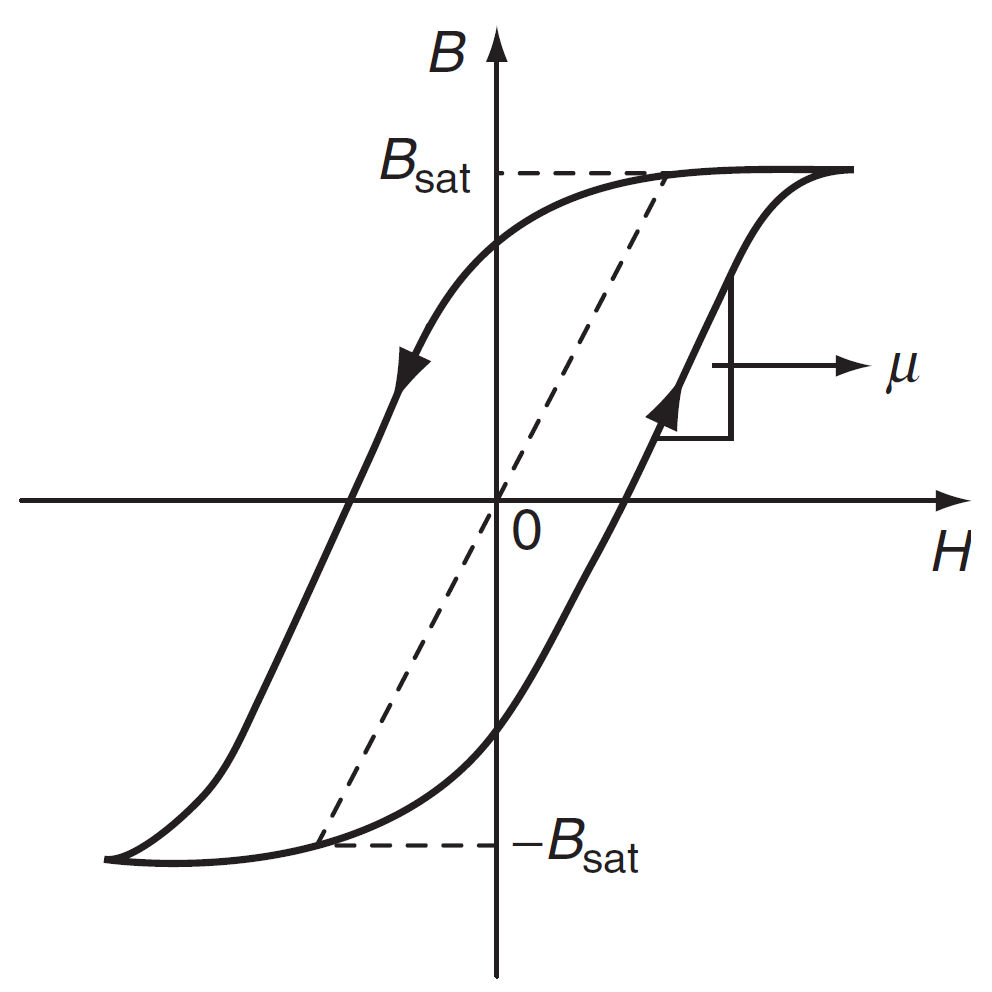
\includegraphics[width=0.7\linewidth]{fig/lec07/practical_BH_loop.png} 
                \caption{Practical $B$--$H$ loop showing hysteresis. Adapted from Umanand, \textit{Power Electronics: Essentials and Applications}, 2nd edition, Wiley, 2012.}
            \end{figure} 
            The core-loss energy density per cycle is proportional to 
            \begin{align} 
                W_{\mathrm{hyst}} \propto \oint H\,dB 
            \end{align} 
        \end{column} 
    \end{columns} 
\end{frame}


%%%%%%%%%%%%%%%%%%%%%%%%%%%%%%%%%%%%%%%%%%%%%%%%%%%%%%%%%%%%% %% Saturation flux density %%%%%%%%%%%%%%%%%%%%%%%%%%%%%%%%%%%%%%%%%%%%%%%%%%%%%%%%%%%%%
\begin{frame} 
    \frametitle{Saturation Flux Density of Magnetic Materials} 
    \begin{columns} 
        \begin{column}{0.56\textwidth} 
            The saturation flux density $B_{\mathrm{sat}}$ is a key material limit. If the operating flux density approaches this value, the effective permeability collapses and the magnetic component can no longer behave as intended. 
            \vspace{0.15cm} 
            \begin{table} 
                \centering 
                \small 
                \begin{tabular}{lc} 
                    \hline 
                    \textbf{Core material} & \textbf{Typical $B_{\mathrm{sat}}$}\\ 
                    \hline 
                    Ferrite & $\approx 0.3\ \si{\tesla}$\\
                    Silicon steel & $\approx 1.0$--$1.2\ \si{\tesla}$\\ 
                    Powdered iron & $\approx 1.6\ \si{\tesla}$\\ 
                    Amorphous core & $\approx 1.6\ \si{\tesla}$\\ 
                    Mu-metal & $\approx 1.0\ \si{\tesla}$\\ \hline 
                \end{tabular} 
            \end{table} 
            \vspace{0.1cm} 
            These values provide first-order design limits. Practical operation usually uses lower peak flux density to limit core loss and temperature rise. 
        \end{column} 
        \begin{column}{0.40\textwidth} 
            \begin{block}{Power Electronics Interpretation} 
                \small High $B_{\mathrm{sat}}$ enables smaller cores, but high-frequency operation is often limited more strongly by core loss than by saturation. Ferrites have lower $B_{\mathrm{sat}}$, but are widely used at high frequency because of their relatively low eddy-current loss. 
            \end{block} 
         \end{column} 
    \end{columns} 
\end{frame}

%%%%%%%%%%%%%%%%%%%%%%%%%%%%%%%%%%%%%%%%%%%%%%%%%%%%%%%%%%%%% %% Reluctance %%%%%%%%%%%%%%%%%%%%%%%%%%%%%%%%%%%%%%%%%%%%%%%%%%%%%%%%%%%%%
\begin{frame} 
    \frametitle{Reluctance: Opposition to Magnetic Flux} 
    \begin{columns} 
        \begin{column}{0.58\textwidth} 
            In an electrical circuit, resistance opposes current flow. Similarly, in a magnetic circuit, reluctance opposes magnetic flux. 
            Starting from 
                $H=\frac{Ni}{l_m}$ and $B=\mu H$ 
            with $\Phi=BA_c$, one obtains 
            \begin{align} 
                \Phi = \frac{Ni\,\mu A_c}{l_m} 
            \end{align} or 
            \begin{align} 
                \Phi = \frac{F}{\mathcal R} 
            \end{align} 
            where $\mathcal R = \frac{l_m}{\mu A_c}$ is called the magnetic reluctance.
            \begin{itemize}
                \item Long magnetic paths increase reluctance. 
                \item Large core area reduces reluctance. 
                \item High permeability reduces reluctance. 
            \end{itemize} 
        \end{column} 
        \begin{column}{0.38\textwidth} 
            \begin{block}{Electrical Analogy} 
                \begin{align} 
                    I=\frac{V}{R} 
                \end{align} 
                \begin{align} 
                    \Phi=\frac{F}{\mathcal R} 
                \end{align} 
            \end{block} 
            \begin{itemize} 
                \item Voltage $\leftrightarrow$ MMF 
                \item Current $\leftrightarrow$ Flux 
                \item Resistance $\leftrightarrow$ Reluctance 
            \end{itemize} 
        \end{column} 
    \end{columns} 
\end{frame}


%%%%%%%%%%%%%%%%%%%%%%%%%%%%%%%%%%%%%%%%%%%%%%%%%%%%%%%%%%%%% %% Permeance %%%%%%%%%%%%%%%%%%%%%%%%%%%%%%%%%%%%%%%%%%%%%%%%%%%%%%%%%%%%%
\begin{frame} 
    \frametitle{Permeance: Ease of Magnetic Flux Flow} 
    \begin{columns} 
        \begin{column}{0.58\textwidth} 
            The reciprocal of reluctance is called permeance. 
            \begin{align} 
                \Lambda = \frac{1}{\mathcal R} 
            \end{align} 
            Substituting the reluctance expression gives 
                $\Lambda = \frac{\mu A_c}{l_m}$ 
            Therefore $
                \Phi=\Lambda F $
                Permeance describes how easily magnetic flux can be established within a magnetic path. 
                \begin{itemize} 
                    \item Large cross-sectional area increases permeance. 
                    \item High permeability materials increase permeance. 
                    \item Longer magnetic paths decrease permeance. 
                \end{itemize} 
            \end{column} 
            \begin{column}{0.38\textwidth} 
                \begin{block}{Electrical Analogy} 
                    Conductance: 
                    \begin{align} 
                        G=\frac{1}{R} 
                    \end{align} 
                    Magnetic equivalent: 
                    \begin{align} 
                        \Lambda=\frac{1}{\mathcal R} 
                    \end{align} 
                \end{block} 
                Permeance plays a role analogous to capacitance in the magnetic energy-storage viewpoint discussed. 
        \end{column} 
    \end{columns} 
\end{frame}

%%%%%%%%%%%%%%%%%%%%%%%%%%%%%%%%%%%%%%%%%%%%%%%%%%%%%%%%%%%%% %% Magnetic circuits %%%%%%%%%%%%%%%%%%%%%%%%%%%%%%%%%%%%%%%%%%%%%%%%%%%%%%%%%%%%% 
\begin{frame} 
    \frametitle{Magnetic Circuit Representation} 
    \begin{columns} 
        \begin{column}{0.58\textwidth} 
            Magnetic components are often represented using equivalent magnetic circuits. 
            \vspace{0.15cm} 
            The governing magnetic-circuit equation is 
            \begin{align} 
                F=\Phi\mathcal R 
            \end{align} 
            \vspace{0.15cm} 
            Using this representation: 
            \begin{itemize} 
                \item Flux can be calculated using circuit techniques. 
                \item Air gaps can be incorporated naturally. 
                \item Core saturation can be interpreted physically. 
                \item Inductance calculations become straightforward. 
            \end{itemize} 
        \end{column} 
        \begin{column}{0.38\textwidth} 
            \begin{figure} 
                \centering 
                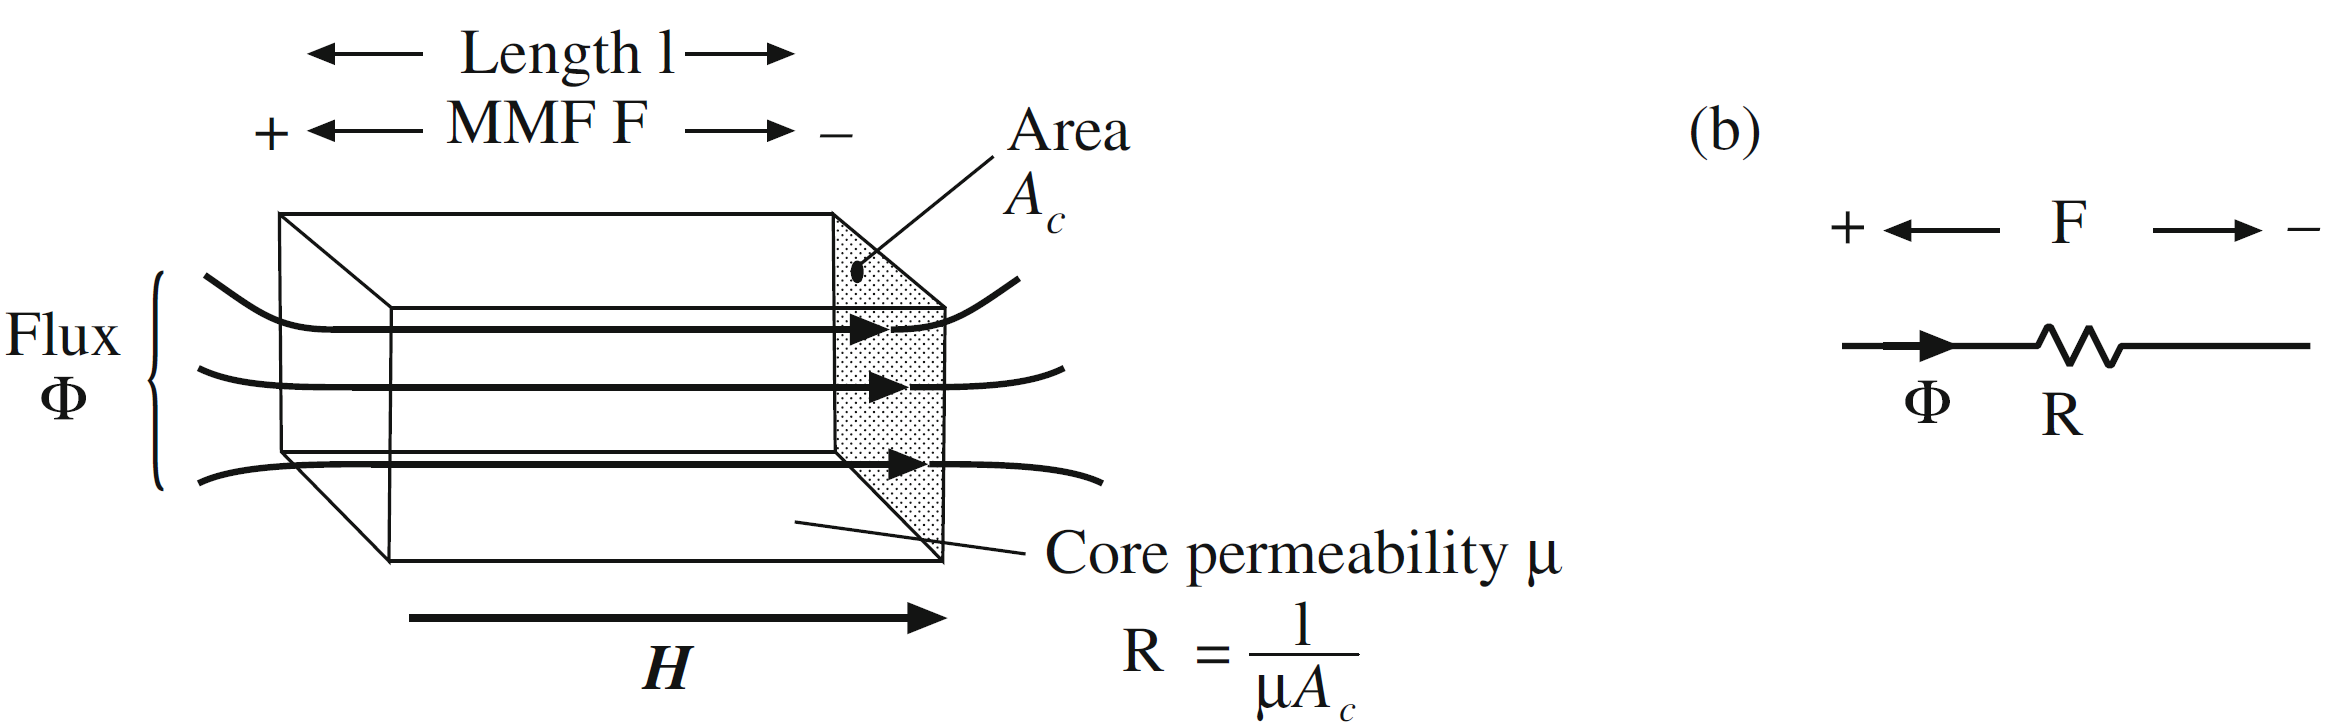
\includegraphics[width=\linewidth]{fig/lec07/magnetic_circuit_equivalent.png} 
                \caption{Equivalent magnetic circuit representation of a magnetic core. Adapted from Erickson and Maksimovi\'c, \textit{Fundamentals of Power Electronics}, 3rd edition, Springer, 2013.}
            \end{figure} 
        \end{column} 
    \end{columns} 
\end{frame}

%%%%%%%%%%%%%%%%%%%%%%%%%%%%%%%%%%%%%%%%%%%%%%%%%%%%%%%%%%%%% %% Series magnetic circuit %%%%%%%%%%%%%%%%%%%%%%%%%%%%%%%%%%%%%%%%%%%%%%%%%%%%%%%%%%%%%
\begin{frame} 
    \frametitle{Series Magnetic Circuits} 
    \begin{columns} 
        \begin{column}{0.58\textwidth} 
            When magnetic flux passes sequentially through several sections of a magnetic path, the corresponding reluctances are connected in series. 
            \begin{align} 
                \mathcal R_{eq} = \mathcal R_1 + \mathcal R_2 + \mathcal R_3 +\cdots 
            \end{align} 
            The same magnetic flux flows through all sections: 
            \begin{align} 
                \Phi_1=\Phi_2=\Phi_3 
            \end{align} 
            The total MMF is 
            \begin{align} 
                F=\Phi \mathcal R_{eq} 
            \end{align} 
            \vspace{0.15cm}  
        \end{column} 
        \begin{column}{0.38\textwidth} 
            \begin{block}{Electrical Equivalent} 
                \begin{align} 
                    R_{eq}=R_1+R_2+R_3 
                \end{align} 
            \end{block} 
            \vspace{0.2cm} 
            Exactly the same mathematical rules apply to reluctances. Examples: 
            \begin{itemize} 
                \item Core section + air gap. 
                \item Multi-material magnetic path. 
                \item Practical transformer cores. 
            \end{itemize}
        \end{column} 
    \end{columns} 
\end{frame}


%%%%%%%%%%%%%%%%%%%%%%%%%%%%%%%%%%%%%%%%%%%%%%%%%%%%%%%%%%%%% %% Air gap reluctance %%%%%%%%%%%%%%%%%%%%%%%%%%%%%%%%%%%%%%%%%%%%%%%%%%%%%%%%%%%%%
\begin{frame} 
    \frametitle{Why Does the Air Gap Dominate Reluctance?} 
    \begin{columns} 
        \begin{column}{0.58\textwidth} 
            Consider a magnetic core containing a small air gap $l_g$. The total reluctance becomes 
            \begin{align} 
                \mathcal R = \frac{l_m}{\mu_0\mu_r A_c} + \frac{l_g}{\mu_0A_c} 
            \end{align} 
            Since 
                $\mu_r \gg 1$ 
            for practical magnetic materials, 
            \begin{align} 
                \mathcal R \approx \frac{l_g}{\mu_0A_c} 
            \end{align} 
            \vspace{0.15cm} 
            Therefore: 
            \begin{itemize} 
                \item Even a very small air gap dominates the total reluctance. 
                \item The effective permeability decreases dramatically. 
                \item Saturation current increases significantly. 
            \end{itemize} 
        \end{column} 
        \begin{column}{0.38\textwidth} 
            \begin{figure} 
                \centering 
                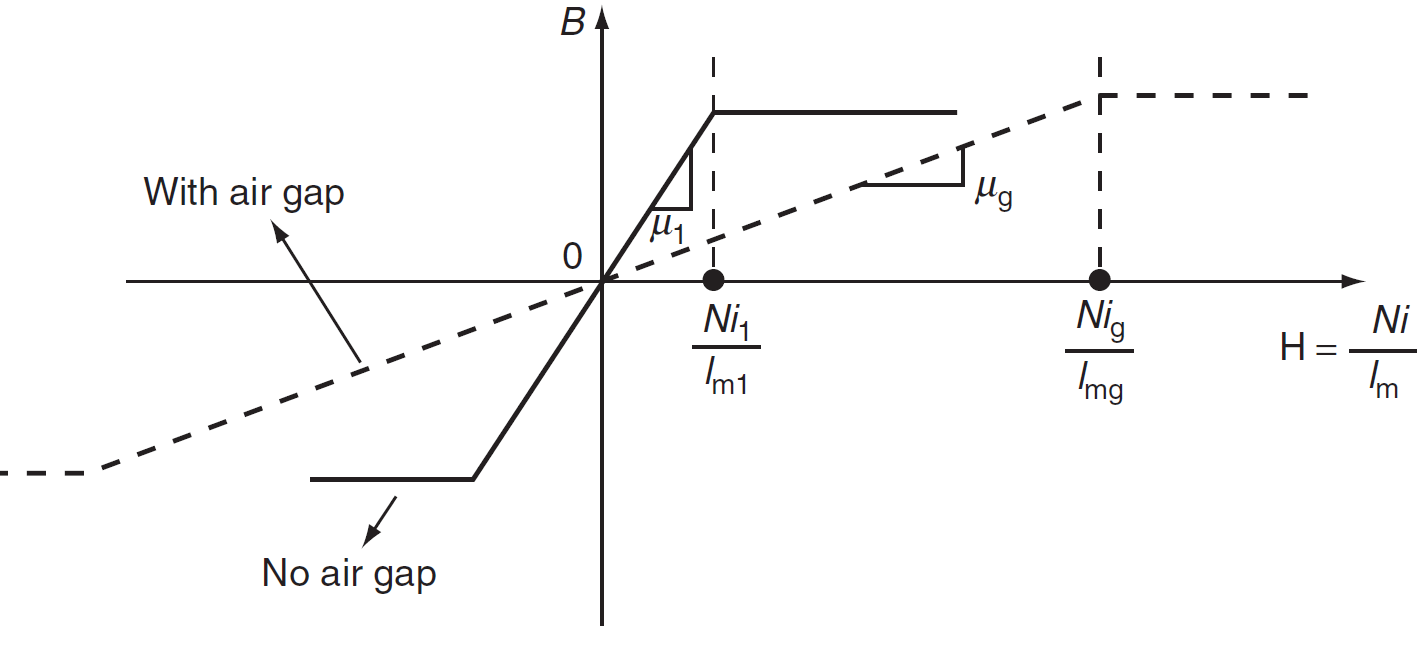
\includegraphics[width=\linewidth]{fig/lec07/air_gap_effect.png} 
                \caption{Effect of air-gap introduction on magnetic characteristics. Adapted from Umanand, \textit{Power Electronics: Essentials and Applications}, 2nd edition, Wiley, 2012.}
            \end{figure} 
        \end{column} 
    \end{columns} 
\end{frame}

%%%%%%%%%%%%%%%%%%%%%%%%%%%%%%%%%%%%%%%%%%%%%%%%%%%%%%%%%%%%% %% Flux division %%%%%%%%%%%%%%%%%%%%%%%%%%%%%%%%%%%%%%%%%%%%%%%%%%%%%%%%%%%%% 
\begin{frame} 
    \frametitle{Parallel Magnetic Circuits and Flux Division} 
    \begin{columns} 
        \begin{column}{0.58\textwidth} 
            Just as electric current divides among parallel resistors, magnetic flux divides among parallel reluctance paths. 
            \vspace{0.15cm} 
            For two parallel paths, 
            \begin{align} 
                \Phi = \Phi_1+\Phi_2 \quad F_1=F_2 
            \end{align}
            The flux distribution becomes 
            \begin{align} 
                \Phi_1 = \frac{F}{\mathcal R_1} 
            \end{align} 
            \begin{align} 
                \Phi_2 = \frac{F}{\mathcal R_2} 
            \end{align} 
            Flux naturally prefers the lower-reluctance path. 
        \end{column} 
        \begin{column}{0.38\textwidth} 
            \begin{block}{Important Observation} 
                High-permeability materials attract magnetic flux. 
                This principle explains: 
                \begin{itemize} 
                    \item Magnetic shielding 
                    \item Flux concentrators 
                    \item Core shaping 
                    \item Leakage-flux paths 
                \end{itemize} 
            \end{block} 
        \end{column} 
    \end{columns} 
\end{frame}


%%%%%%%%%%%%%%%%%%%%%%%%%%%%%%%%%%%%%%%%%%%%%%%%%%%%%%%%%%%%% %% Volt second balance %%%%%%%%%%%%%%%%%%%%%%%%%%%%%%%%%%%%%%%%%%%%%%%%%%%%%%%%%%%%% 
\begin{frame} 
    \frametitle{Volt-Second Balance: Fundamental Principle} 
    \begin{columns} 
        \begin{column}{0.58\textwidth} 
            Starting from Faraday's law, 
            \begin{align} 
                v=N A_c\frac{dB}{dt} 
            \end{align} 
            Integrating over one switching period, 
            \begin{align} 
                \int_0^T v(t)dt = NA_c \int_0^T dB 
            \end{align} 
            For periodic steady-state operation, 
            \begin{align} 
                B(T)=B(0) 
            \end{align} 
            Therefore, is the volt-second balance condition: 
            \begin{align} 
                \int_0^T v(t)dt=0 
            \end{align} 
        \end{column} 
        \begin{column}{0.38\textwidth} 
            \begin{block}{Physical Meaning} The average voltage across a magnetic winding must be zero in steady state. Otherwise flux continues to accumulate cycle after cycle. 
            \end{block} 
        \end{column} 
    \end{columns} 
\end{frame}

%%%%%%%%%%%%%%%%%%%%%%%%%%%%%%%%%%%%%%%%%%%%%%%%%%%%%%%%%%%%% %% Volt second and saturation %%%%%%%%%%%%%%%%%%%%%%%%%%%%%%%%%%%%%%%%%%%%%%%%%%%%%%%%%%%%% 
\begin{frame} 
    \frametitle{Flux Build-Up and Core Saturation} 
    \begin{columns} 
        \begin{column}{0.58\textwidth} 
            From \begin{align} B = \frac{1}{NA_c} \int v(t)dt 
            \end{align} 
            we observe that flux density is determined by the accumulated volt-seconds. 
            \vspace{0.15cm} 
            If 
            \begin{align} 
                \frac{1}{T} \int_0^T v(t)dt \neq 0 
            \end{align} 
            then $B \rightarrow \infty$ in the ideal mathematical model. Practically, the flux density reaches 
            \begin{align} 
                B_{sat} 
            \end{align} 
            and the core saturates. 
        \end{column} 
        \begin{column}{0.38\textwidth} 
            \begin{block}{Design Implication} 
                A transformer can saturate even at low load current if volt-second balance is violated. 
                \vspace{0.15cm} 
                Transformer saturation is governed primarily by flux density, not by output current. 
            \end{block} 
        \end{column} 
    \end{columns} 
\end{frame}

%%%%%%%%%%%%%%%%%%%%%%%%%%%%%%%%%%%%%%%%%%%%%%%%%%%%%%%%%%%%% %% Volt second example %%%%%%%%%%%%%%%%%%%%%%%%%%%%%%%%%%%%%%%%%%%%%%%%%%%%%%%%%%%%% 
\begin{frame} 
    \frametitle{Example: Volt-Second Balance in a Square-Wave Excitation} 
    \begin{columns} 
        \begin{column}{0.58\textwidth} 
            Consider a winding excited by 
            \begin{align} +V \quad \mathrm{for}\quad \frac{T}{2} \quad \text{and} \quad -V \quad \mathrm{for}\quad \frac{T}{2} 
            \end{align} 
            The total volt-seconds become 
            \begin{align} 
                VT/2 - VT/2 =0 
            \end{align} 
            Hence, 
            \begin{itemize} 
                \item Flux oscillates around zero. 
                \item No long-term flux accumulation occurs. 
                \item Core saturation is avoided. 
            \end{itemize} 
            This is the operating principle of ideal transformer excitation. 
        \end{column} 
        \begin{column}{0.38\textwidth} 
            \begin{figure} 
                \centering 
                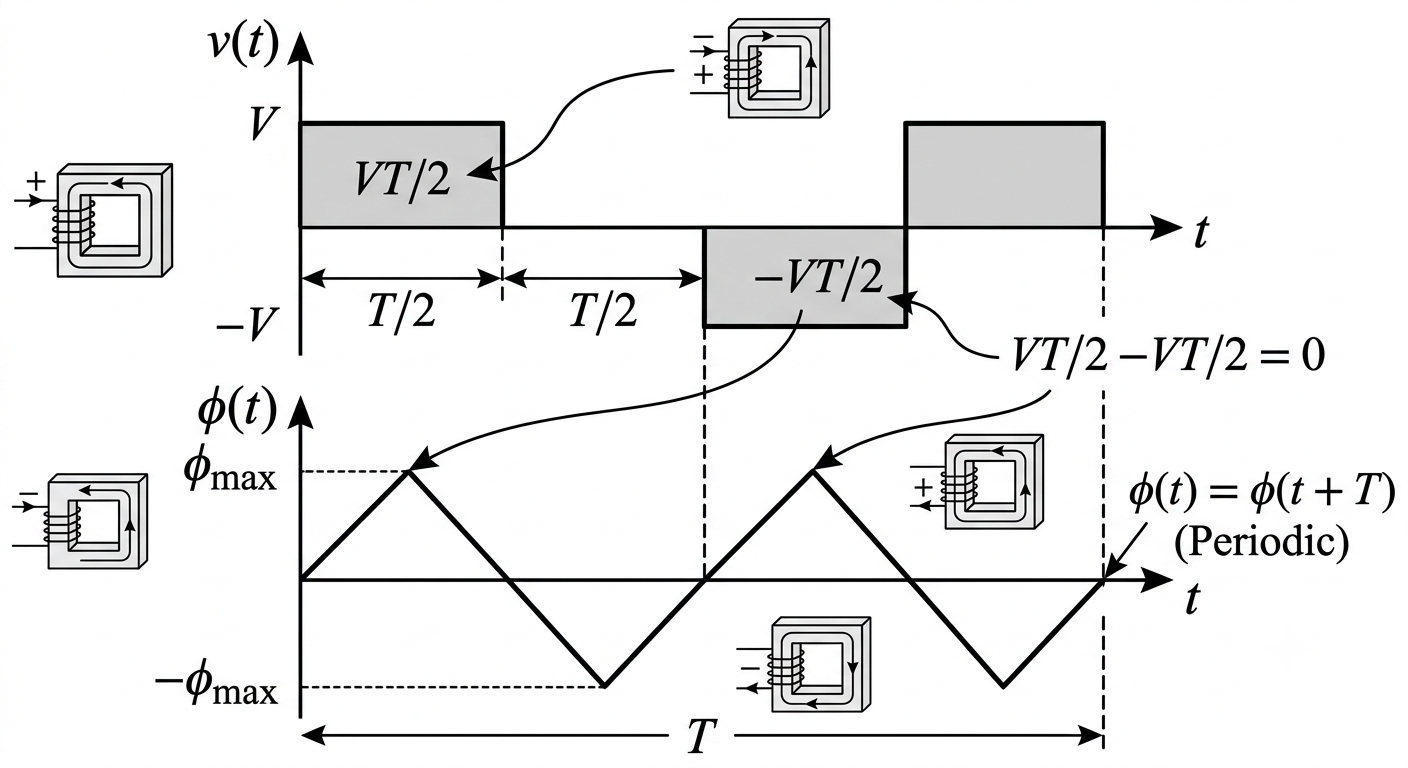
\includegraphics[width=\linewidth]{fig/lec07/square_wave_volt_second_balance.png} 
                \caption{Balanced positive and negative volt-seconds leading to periodic flux excursion.} 
            \end{figure} 
        \end{column} 
    \end{columns} 
\end{frame}

% %%%%%%%%%%%%%%%%%%%%%%%%%%%%%%%%%%%%%%%%%%%%%%%%%%%%%%%%%%%%% %% Inductor concept %%%%%%%%%%%%%%%%%%%%%%%%%%%%%%%%%%%%%%%%%%%%%%%%%%%%%%%%%%%%%
% \begin{frame} 
%     \frametitle{What is an Inductor?} 
%     \begin{columns} 
%         \begin{column}{0.58\textwidth} 
%             An inductor is a magnetic component that stores energy in its magnetic field when current flows through its winding. 
%             \vspace{0.15cm} Unlike transformers, which ideally transfer energy from one winding to another, inductors are specifically designed to store energy temporarily. 
%             \vspace{0.15cm} 
%             Typical applications include: 
%             \begin{itemize} 
%                 \item Buck converters 
%                 \item Boost converters 
%                 \item Flyback converters 
%                 \item EMI filters 
%                 \item Resonant converters 
%                 \item Motor drives 
%             \end{itemize} 
%             \vspace{0.15cm} 
%         \end{column} 
%         \begin{column}{0.38\textwidth} 
%             The electrical behaviour of an inductor is governed by 
%             \begin{align} 
%                 v=L\frac{di}{dt} 
%             \end{align} 
%             which indicates that an inductor opposes changes in current. 
%             \begin{block}{Physical Interpretation} 
%                 Current establishes magnetic flux. 
%                 \vspace{0.1cm} 
%                 The magnetic field stores energy and resists abrupt changes in current. 
%             \end{block} 
%         \end{column} 
%     \end{columns} 
% \end{frame}


% %%%%%%%%%%%%%%%%%%%%%%%%%%%%%%%%%%%%%%%%%%%%%%%%%%%%%%%%%%%%% %% Inductor derivation %%%%%%%%%%%%%%%%%%%%%%%%%%%%%%%%%%%%%%%%%%%%%%%%%%%%%%%%%%%%%
% \begin{frame} 
%     \frametitle{Derivation of Inductance from Magnetic Circuits} 
%     \begin{columns} 
%         \begin{column}{0.58\textwidth} 
%             Starting from the magnetic circuit relation 
%                 $\Phi=\Lambda Ni$.
%             Differentiating with respect to time, 
%             \begin{align} 
%                 \frac{d\Phi}{dt} = \Lambda N \frac{di}{dt} 
%             \end{align} 
%             Applying Faraday's law, 
%             \begin{align} 
%                 v = N\frac{d\Phi}{dt} \text{yields} \quad v = \Lambda N^2 \frac{di}{dt}
%             \end{align} 
%             Comparing with 
%             \begin{align} 
%                 v=L\frac{di}{dt} \quad \Longrightarrow \quad L=\Lambda N^2
%             \end{align} 
%         \end{column} 
%         \begin{column}{0.38\textwidth} 
%             \begin{block}{Important Result} 
%                 \begin{align} 
%                     L=\Lambda N^2 
%                 \end{align} 
%                 \vspace{0.1cm} 
%                 Inductance is determined by \begin{itemize} \item Number of turns \item Core geometry \item Core permeability \item Air gap \end{itemize} 
%             \end{block} 
%         \end{column} 
%     \end{columns} 
% \end{frame}

%%%%%%%%%%%%%%%%%%%%%%%%%%%%%%%%%%%%%%%%%%%%%%%%%%%%%%%%%%%%% %% Physical inductance %%%%%%%%%%%%%%%%%%%%%%%%%%%%%%%%%%%%%%%%%%%%%%%%%%%%%%%%%%%%% 
\begin{frame} 
    \frametitle{Physical Expression for Inductance} 
    \begin{columns} 
        \begin{column}{0.58\textwidth} 
            Substituting 
                $\Lambda=\frac{\mu A_c}{l_m}$ 
            into $
                L=\Lambda N^2 $
            gives 
            \begin{align} 
                L= \frac{\mu A_c N^2}{l_m} 
            \end{align} 
            This expression reveals the physical parameters that determine inductance. 
            \vspace{0.15cm} 
            \begin{itemize} 
                \item Increasing turns increases inductance quadratically. 
                \item Increasing permeability increases inductance. 
                \item Increasing core area increases inductance. 
                \item Increasing magnetic path length reduces inductance. 
            \end{itemize} 
        \end{column} 
        \begin{column}{0.38\textwidth} 
            \begin{block}{Design Insight} 
                \begin{align} 
                    L \propto N^2 
                \end{align} 
                Doubling the number of turns increases inductance by a factor of four. 
            \end{block} 
        \end{column} 
    \end{columns} 
\end{frame}


%%%%%%%%%%%%%%%%%%%%%%%%%%%%%%%%%%%%%%%%%%%%%%%%%%%%%%%%%%%%% %% Energy storage %%%%%%%%%%%%%%%%%%%%%%%%%%%%%%%%%%%%%%%%%%%%%%%%%%%%%%%%%%%%% 
\begin{frame} 
    \frametitle{Energy Stored in an Inductor} 
    \begin{columns} 
        \begin{column}{0.58\textwidth} 
            The energy stored in an inductor is 
            \begin{align} 
                E_L = \int vi\,dt 
            \end{align} 
            Substituting 
                $v=L\frac{di}{dt}$ 
            gives 
            \begin{align} 
                E_L = \int Li\,di 
            \end{align} 
            which yields 
            \begin{align} 
                E_L = \frac12 LI^2 
            \end{align} 
            \vspace{0.15cm} 


        \end{column} 
        \begin{column}{0.38\textwidth}
            Key observations:  
            \begin{itemize} 
                \item Energy increases with current squared. 
                \item Energy is recoverable. 
                \item Inductors are energy-storage devices. 
                \item Larger currents require significantly larger stored energy capability. 
            \end{itemize} 
            \begin{block}{Example} 
                If $L=100\ \mu H $ and $I=10A$ then $E_L=5\,mJ$ 
            \end{block} 
        \end{column} 
    \end{columns} 
\end{frame}


%%%%%%%%%%%%%%%%%%%%%%%%%%%%%%%%%%%%%%%%%%%%%%%%%%%%%%%%%%%%% %% Energy storage physical meaning %%%%%%%%%%%%%%%%%%%%%%%%%%%%%%%%%%%%%%%%%%%%%%%%%%%%%%%%%%%%% 
\begin{frame} 
    \frametitle{Where is the Energy Actually Stored?} 
    \begin{columns} 
        \begin{column}{0.58\textwidth} 
            A common misconception is that energy is stored in the magnetic core. 
            \vspace{0.15cm} 
            In reality, energy is stored in the magnetic field itself. 
            \vspace{0.15cm} 
            The magnetic energy density is 
            \begin{align} 
                w_m = \frac12 BH 
            \end{align} 
            and total stored energy becomes 
            \begin{align} 
                E=\int_V \frac12 BH\,dV 
            \end{align} 
            \vspace{0.15cm} 
            For gapped inductors: 
            \begin{itemize} 
                \item Most stored energy resides in the air gap. 
                \item The magnetic core primarily guides flux. 
                \item The air gap acts as the main energy-storage region. 
            \end{itemize} 
        \end{column} 
        \begin{column}{0.38\textwidth} 
            \begin{block}{Important Concept} 
                Transformer \[ \text{Transfer energy} \] 
                Inductor \[ \text{Store energy} \] 
                This distinction drives completely different magnetic designs. 
            \end{block} 
        \end{column} 
    \end{columns} 
\end{frame}



\begin{frame}{Magnetic Materials Used in Power Electronics}
Magnetic materials are selected according to the operating frequency, allowable flux density, core loss and cost. No single material is optimal for all applications.
\begin{table}
\centering
\footnotesize
\begin{tabular}{lccc}
\toprule
Material & Typical $B_{\mathrm{sat}}$ & Frequency Range & Typical Applications\\
\midrule
Silicon steel & 1.0--2.0 T & 50--400 Hz & Grid transformers\\
Ferrite & 0.25--0.5 T & 20 kHz--2 MHz & SMPS, LLC, Flyback\\
Powdered iron & 0.6--1.6 T & up to $\sim$500 kHz & PFC inductors\\
Amorphous alloy & 0.8--1.5 T & kHz range & High-efficiency transformers\\
Nanocrystalline & 1.1--1.3 T & up to MHz & EV, aerospace magnetics\\
\bottomrule
\end{tabular}
\end{table}

\begin{block}{Design Insight}
High-frequency converters generally favour ferrite cores because their extremely high electrical resistivity suppresses eddy-current loss, even though their saturation flux density is relatively low. Conversely, silicon-steel cores offer much higher saturation flux density but become unsuitable
for high-frequency operation due to excessive core loss.
\end{block}
\end{frame}

\begin{frame}{Core Loss versus Frequency}
    \begin{columns} 
        \begin{column}{0.58\textwidth}
Core loss increases rapidly with switching frequency.
Two physical mechanisms contribute:

\begin{itemize}
\item \textbf{Hysteresis loss} caused by repeated reversal of magnetic domains.
\item \textbf{Eddy-current loss} caused by induced circulating currents inside the core.
\end{itemize}

The total core loss is commonly approximated using the Steinmetz equation
\[
P_{\mathrm{core}}
=
k
f^{\alpha}
B_{\mathrm{pk}}^{\beta}
V_{\mathrm{core}}
\]
\begin{itemize}
\item $f$ is switching frequency,
\item $B_{\mathrm{pk}}$ is peak flux density,
\item $V_{\mathrm{core}}$ is core volume,
\item $k,\alpha,\beta$ are material-dependent constants.
\end{itemize}
\end{column} 

\begin{column}{0.38\textwidth}
            \begin{figure} 
                \centering 
                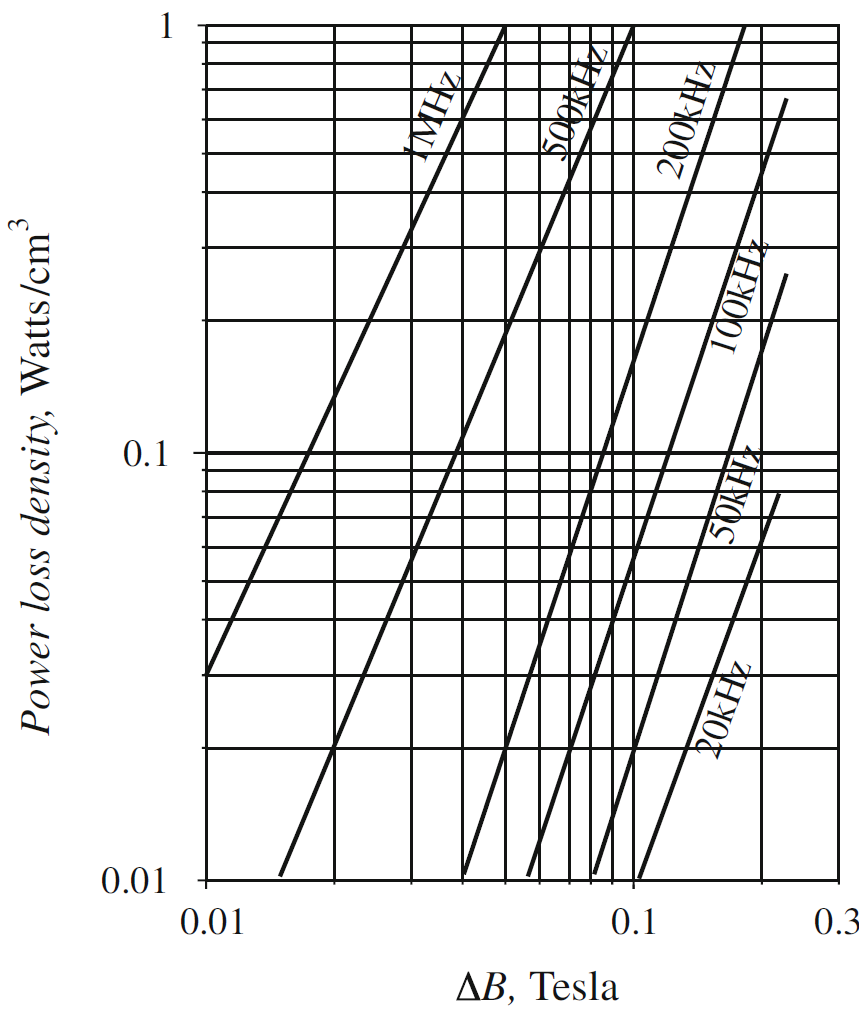
\includegraphics[width=0.65\linewidth]{fig/lec07/Ferrite_loss_curves.png} 
                \caption{Ferrite loss curves and comparison of magnetic materials. Adapted from Erickson \& Maksimović, \textit{Fundamentals of Power Electronics}, 3rd Edition.}
            \end{figure}
\end{column}
\end{columns}
\end{frame}


\begin{frame}{High-Frequency Copper Losses: Skin Effect and Proximity Effect}
At high switching frequencies, winding losses become considerably larger than their DC values.
The increase originates from two electromagnetic phenomena.
\begin{columns}
    \column{0.48\textwidth}
    \textbf{Skin Effect}
    \begin{itemize}
        \item Current crowds near the conductor surface.
        \item Effective conductor area decreases.
        \item AC resistance increases with frequency.
        \item Skin depth
        \[
        \delta=
        \sqrt{\frac{2\rho}{\omega\mu}}
        \]
        determines current penetration.
    \end{itemize}
\column{0.48\textwidth}
    \textbf{Proximity Effect}
    \begin{itemize}
        \item Magnetic fields generated by neighbouring conductors induce eddy currents.
        \item Current distribution becomes highly non-uniform.
        \item AC resistance increases further.
        \item Dominant in multilayer transformer windings.
    \end{itemize}
\end{columns}
\begin{block}{Practical Solution}
Use Litz wire, foil windings or interleaved winding arrangements to minimise AC copper losses.
\end{block}
\end{frame}


\begin{frame}{High-Frequency Copper Losses: Skin Effect and Proximity Effect}
    \begin{columns}
    \column{0.5\textwidth}
            \begin{figure} 
                \centering 
                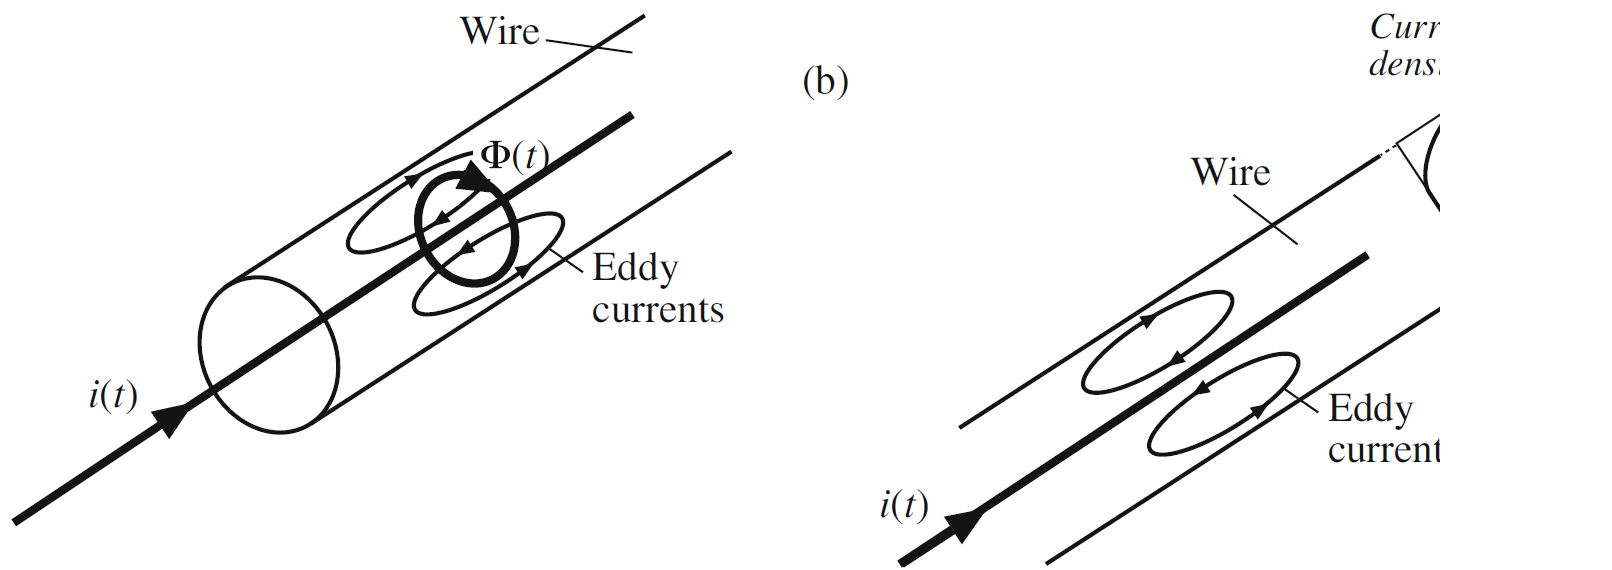
\includegraphics[width=0.9\linewidth]{fig/lec07/skin_effect.png} 
                \caption{Skin effect in conductors at high frequencies. Adapted from Erickson \& Maksimović, \textit{Fundamentals of Power Electronics}, 3rd Edition.}
            \end{figure} 

    \column{0.5\textwidth}
            \begin{figure} 
                \centering 
                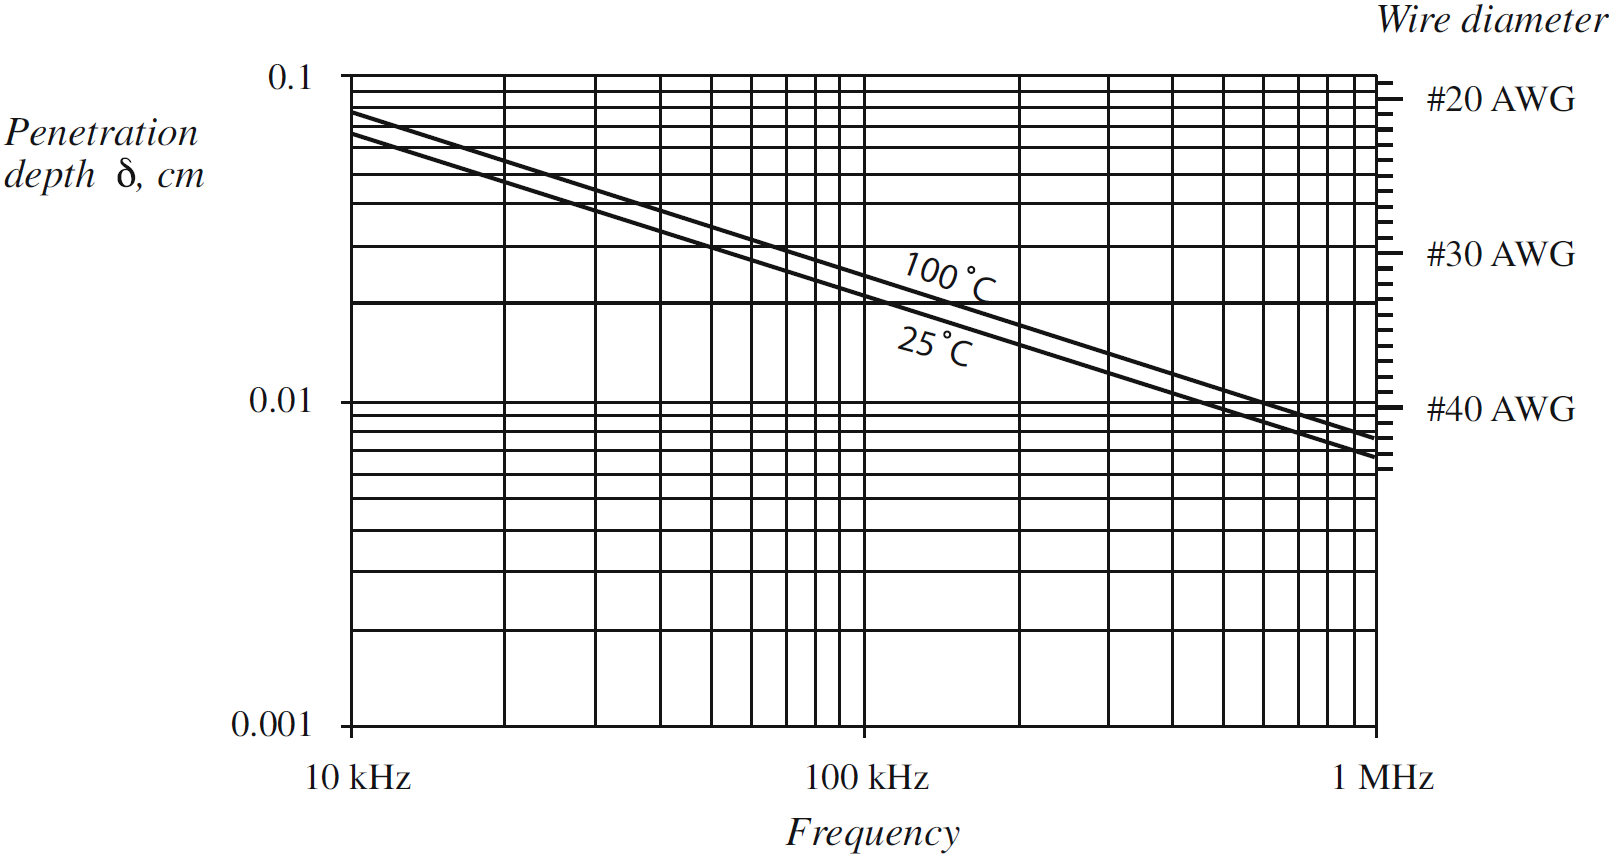
\includegraphics[width=0.9\linewidth]{fig/lec07/penetration_depth.png} 
                \caption{Penetration depth $\delta$ as a function of frequency $f$. Adapted from Erickson \& Maksimović, \textit{Fundamentals of Power Electronics}, 3rd Edition.}
            \end{figure} 
    \end{columns}
\end{frame}



\begin{frame}{High-Frequency Copper Losses: Skin Effect and Proximity Effect}
            \begin{figure} 
                \centering 
                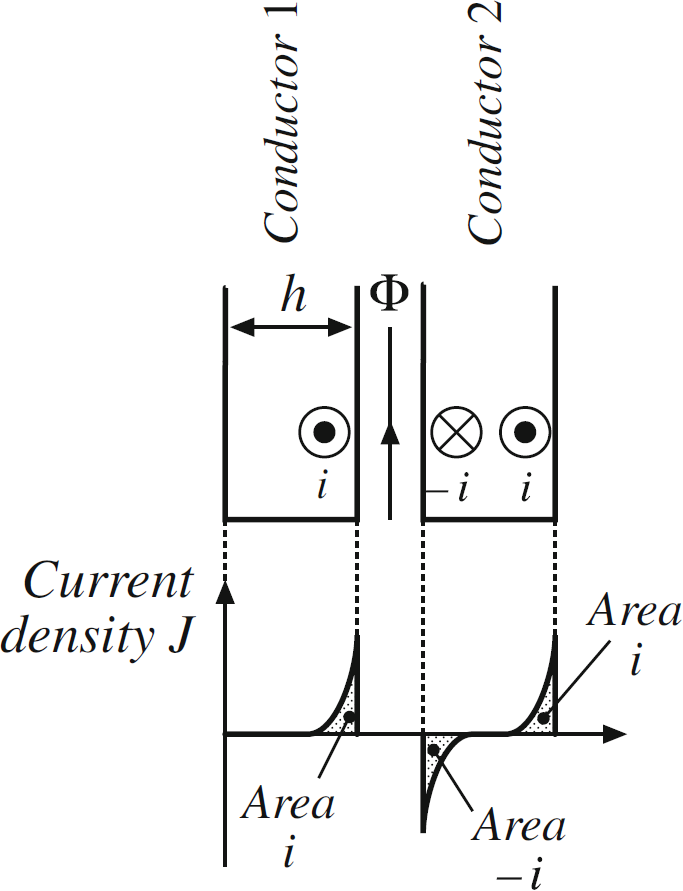
\includegraphics[width=0.275\linewidth]{fig/lec07/proximity_effect.png} 
                \caption{Proximity effect in conductors at high frequencies. Adapted from Erickson \& Maksimović, \textit{Fundamentals of Power Electronics}, 3rd Edition.}
            \end{figure} 
\end{frame}


\begin{frame}{Copper Loss versus Core Loss: Fundamental Design Trade-off}
Magnetic-component design always involves balancing copper loss and core loss.
\begin{columns}
\column{0.52\textwidth}
Increasing the allowable peak flux density $B_{\mathrm{pk}}$ produces
\begin{itemize}
\item fewer turns,
\item shorter winding length,
\item lower copper loss,
\item smaller magnetic component.
\end{itemize}
However,
\[
B_{\mathrm{pk}}
\uparrow
\Rightarrow
P_{\mathrm{core}}
\uparrow
\]
leading to higher temperature rise.
\column{0.44\textwidth}
\begin{block}{Design Objective}
Choose the operating flux density that minimises
\[
P_{\mathrm{total}}
=
P_{\mathrm{core}}
+
P_{\mathrm{copper}}
\]
rather than minimising either loss independently.
\end{block}
\end{columns}
\end{frame}

\begin{frame}{Copper Loss versus Core Loss: Fundamental Design Trade-off}
Magnetic-component design always involves balancing copper loss and core loss.
\begin{columns}
\column{0.3\textwidth}
\begin{alertblock}{Engineering Insight}
Modern GaN and SiC converters often operate at much higher switching frequencies.
Consequently, core loss usually becomes the dominant design constraint, while conventional
low-frequency converters are more frequently limited by copper loss.
\end{alertblock}
\column{0.6\textwidth}
            \begin{figure} 
                \centering 
                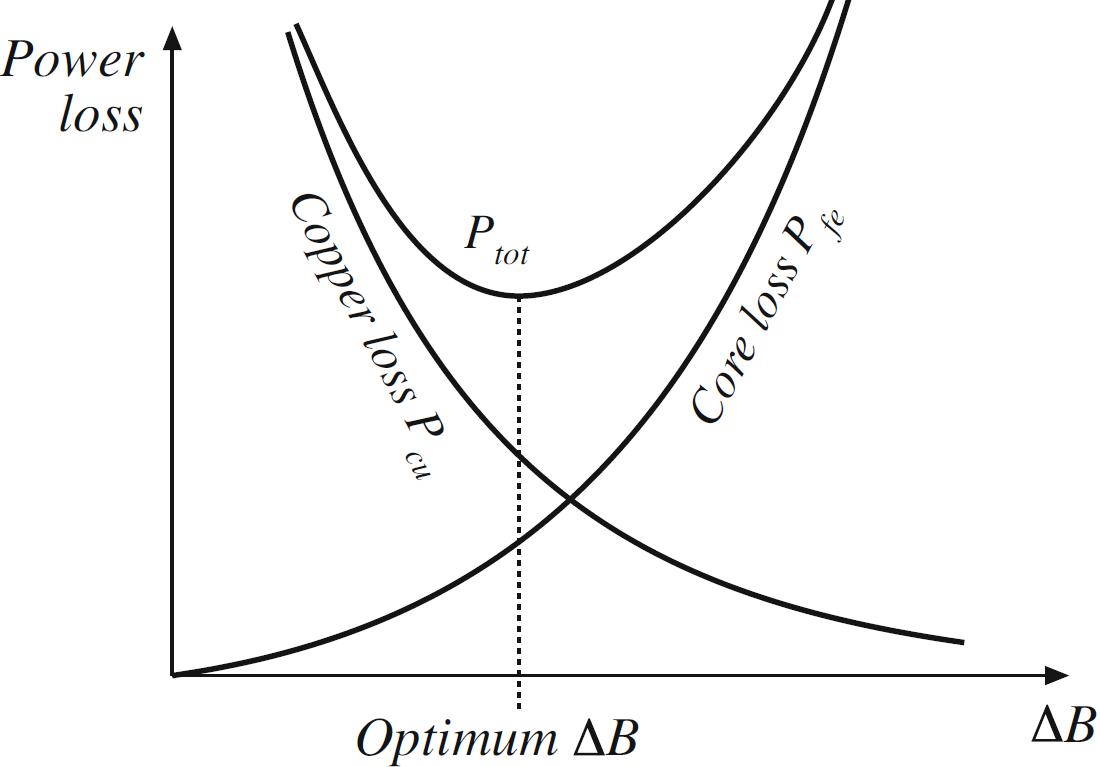
\includegraphics[width=0.8\linewidth]{fig/lec07/loss_curve.png} 
                \caption{Variation of copper loss, core loss and total loss versus peak flux density. Adapted from Erickson \& Maksimović, \textit{Fundamentals of Power Electronics}, 3rd Edition.}
            \end{figure} 
\end{columns}
\end{frame}


% %%%%%%%%%%%%%%%%%%%%%%%%%%%%%%%%%%%%%%%%%%%%%%%%%%%%%%%%%%%%% %% Air gap introduction %%%%%%%%%%%%%%%%%%%%%%%%%%%%%%%%%%%%%%%%%%%%%%%%%%%%%%%%%%%%% 
% \begin{frame} \frametitle{Why are Air Gaps Introduced in Inductors?} 
%     \begin{columns} 
%         \begin{column}{0.58\textwidth} 
%             Power inductors generally require an intentional air gap. 
%             \vspace{0.15cm} 
%             The air gap serves several important functions: 
%             \begin{itemize} 
%                 \item Increases magnetic reluctance. 
%                 \item Reduces effective permeability. 
%                 \item Increases saturation current. 
%                 \item Improves inductance stability. 
%                 \item Enables substantial energy storage. 
%             \end{itemize} 
%             \vspace{0.15cm} 
%             Without an air gap: 
%             \begin{itemize} 
%                 \item Flux density rises rapidly. 
%                 \item Core saturation occurs at relatively low current. 
%             \end{itemize} 
%         \end{column} 
%         \begin{column}{0.38\textwidth} 
%             \begin{figure} 
%                 \centering 
%                 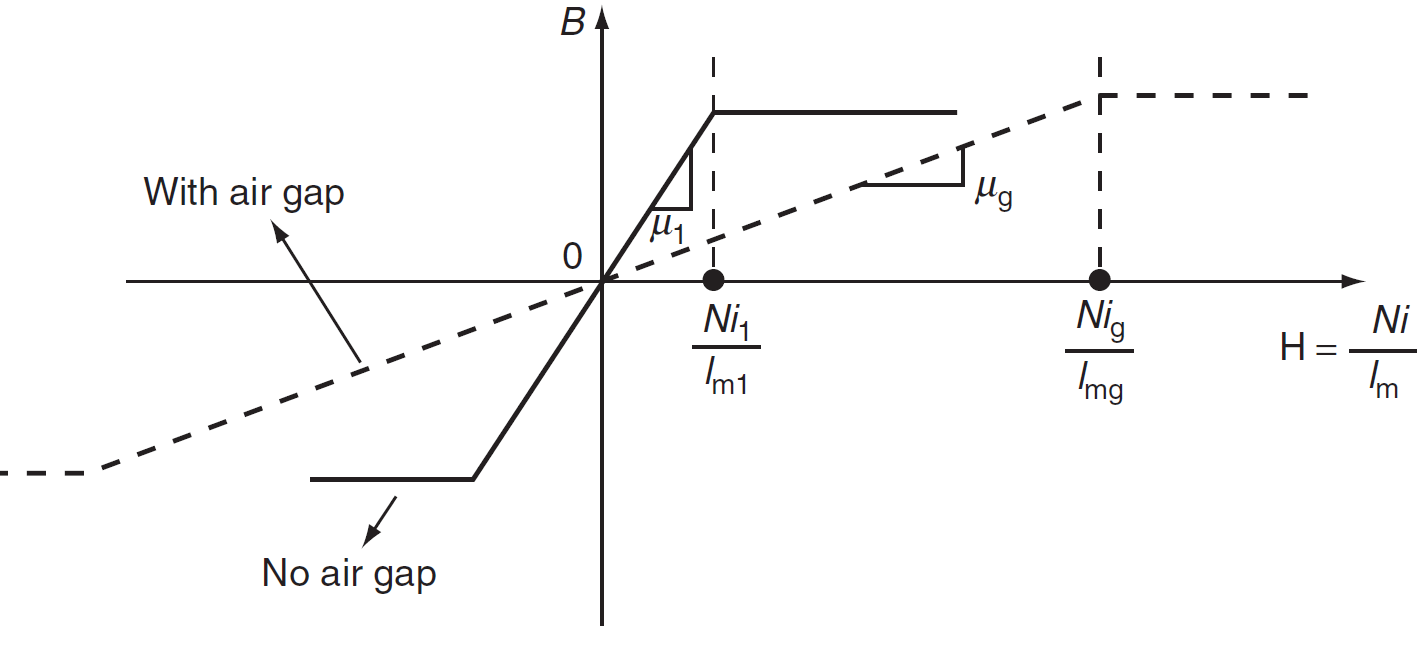
\includegraphics[width=\linewidth]{fig/lec07/air_gap_effect.png} 
%                 \caption{Influence of an air gap on the effective permeability and saturation behaviour. Adapted from Umanand, \textit{Power Electronics: Essentials and Applications}, 2nd edition, Wiley, 2012.}
%             \end{figure} 
%         \end{column} 
%     \end{columns} 
% \end{frame} 

% %%%%%%%%%%%%%%%%%%%%%%%%%%%%%%%%%%%%%%%%%%%%%%%%%%%%%%%%%%%%% %% Air gap and saturation %%%%%%%%%%%%%%%%%%%%%%%%%%%%%%%%%%%%%%%%%%%%%%%%%%%%%%%%%%%%%
% \begin{frame} 
%     \frametitle{Air Gap and Saturation Current} 
%     \begin{columns} 
%         \begin{column}{0.58\textwidth} 
%             The saturation condition occurs when 
%                 $B=B_{sat}$. Using $B=\mu H$ and $               H=\frac{Ni}{l_m} $ one obtains 
%             \begin{align} 
%                 i_{sat} \propto \frac{B_{sat}}{\mu} 
%             \end{align} 
%             \vspace{0.15cm} 
%             Introducing an air gap reduces the effective permeability. Therefore: 
%             \begin{itemize} 
%                 \item Flux density rises more slowly. 
%                 \item Larger current is required to reach saturation. 
%                 \item Energy-storage capability increases. 
%             \end{itemize} 
%         \end{column} 
%         \begin{column}{0.38\textwidth} 
%             \begin{block}{Design Trade-Off} Air gap: 
%                 \begin{itemize} 
%                     \item Higher saturation current 
%                     \item More energy storage 
%                     \item Lower inductance 
%                 \end{itemize} 
%             \end{block} 
%         \end{column} 
%     \end{columns} 
% \end{frame}


%%%%%%%%%%%%%%%%%%%%%%%%%%%%%%%%%%%%%%%%%%%%%%%%%%%%%%%%%%%%% %% Core geometries %%%%%%%%%%%%%%%%%%%%%%%%%%%%%%%%%%%%%%%%%%%%%%%%%%%%%%%%%%%%%
\begin{frame} \frametitle{Magnetic Core Geometries} 
    \begin{columns} 
        \begin{column}{0.56\textwidth} 
            Different core geometries offer different trade-offs in: \vspace{-0.5cm}
            \begin{itemize} 
                \item Winding area 
                \item Leakage flux 
                \item Manufacturability 
                \item Cooling 
                \item Cost 
            \end{itemize} 
            Common geometries include: 
            \begin{itemize} 
                \item EI cores, E cores, C cores, Toroidal cores, PQ cores 
            \end{itemize} 
            Selection depends on frequency, power level, and isolation requirements. 
        \end{column} 
        \begin{column}{0.40\textwidth} 
            \vspace{-1cm}
            \begin{figure} 
                \centering 
                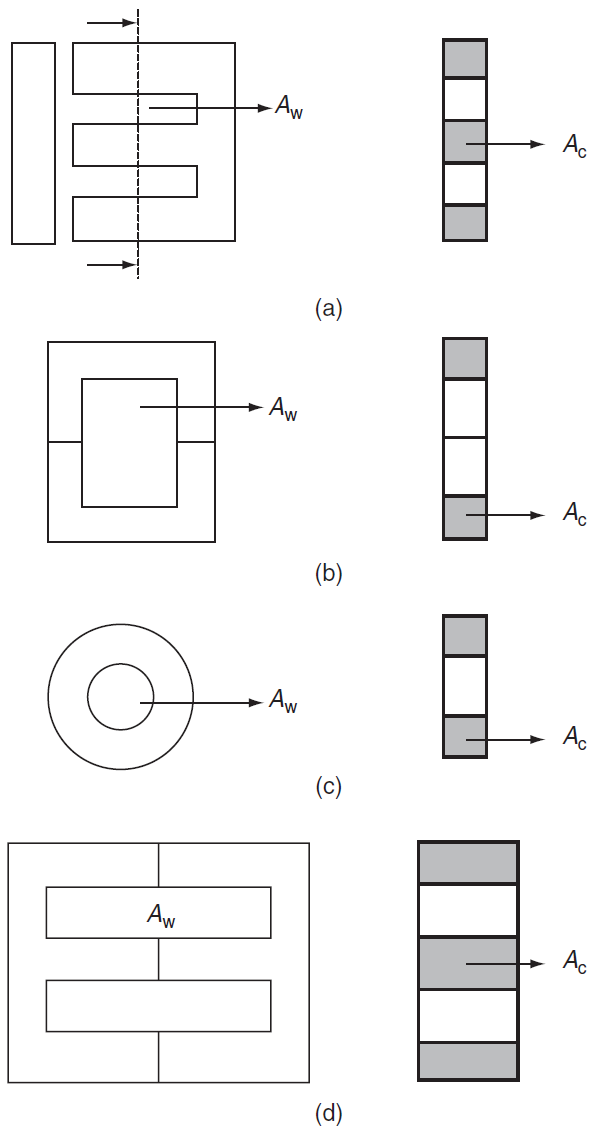
\includegraphics[height=0.68\textheight]{fig/lec07/core_geometries.png} 
                \caption{Window area and cross-sectional area for common magnetic-core geometries. Adapted from Umanand, \textit{Power Electronics: Essentials and Applications}, 2nd edition, Wiley, 2012.}
            \end{figure} 
        \end{column} 
    \end{columns} 
\end{frame} 

%%%%%%%%%%%%%%%%%%%%%%%%%%%%%%%%%%%%%%%%%%%%%%%%%%%%%%%%%%%%% %% Area product %%%%%%%%%%%%%%%%%%%%%%%%%%%%%%%%%%%%%%%%%%%%%%%%%%%%%%%%%%%%%
\begin{frame} 
    \frametitle{Area Product Concept} 
    \begin{columns} 
        \begin{column}{0.58\textwidth} 
            The area-product method provides a simple approach for selecting a magnetic core. 
            \vspace{0.15cm} Two physical parameters are particularly important: 
                $A_c$ 
            Core cross-sectional area and 
                $A_w$. 
            Window area available for windings. Their product 
            \begin{align} 
                A_P=A_cA_w 
            \end{align} is called the area product. 
            \vspace{0.15cm} It links the magnetic core dimensions directly to the electrical design requirements. 
        \end{column} 
        \begin{column}{0.38\textwidth} 
            \begin{block}{Interpretation} \[ A_c \] determines flux capability 
                \vspace{0.1cm} \[ A_w \] determines copper capability 
                \vspace{0.1cm} \[ A_P \] determines overall magnetic capability 
            \end{block} 
        \end{column} 
    \end{columns} 
\end{frame}

%%%%%%%%%%%%%%%%%%%%%%%%%%%%%%%%%%%%%%%%%%%%%%%%%%%%%%%%%%%%% %% Window area %%%%%%%%%%%%%%%%%%%%%%%%%%%%%%%%%%%%%%%%%%%%%%%%%%%%%%%%%%%%%
\begin{frame} \frametitle{Window Area and Copper Accommodation} 
    \begin{columns} 
        \begin{column}{0.58\textwidth} 
            The magnetic core must provide sufficient space to accommodate all winding conductors. 
            \vspace{0.15cm} The available winding space is called the window area: $A_w$. However, the entire window cannot be filled with copper because insulation, bobbins, air spaces, and manufacturing constraints occupy part of the available area. 
                \vspace{0.15cm} 
                Therefore, the usable copper area becomes 
                \begin{align} 
                    A_{Cu} = K_w A_w 
                \end{align} 
                where, $A_w$ = window area and $A_{Cu}$ = total copper area, and $K_w$ is the window utilization factor.
                \vspace{0.15cm} Typical values: $0.2 < K_w < 0.5$ depending on winding complexity. 
            \end{column} 
            \begin{column}{0.38\textwidth} 
                \vspace{-1cm}
                \begin{figure} 
                    \centering 
                    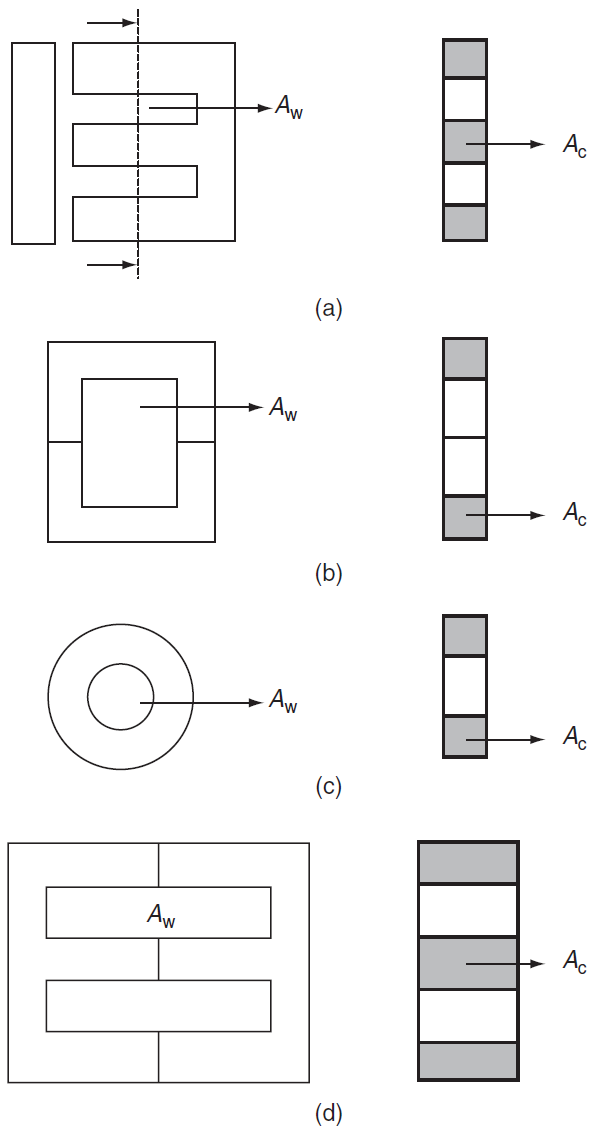
\includegraphics[height=0.68\textheight]{fig/lec07/core_geometries.png} 
                    \caption{Definition of window area $A_w$ and core cross-sectional area $A_c$. Adapted from Umanand, \textit{Power Electronics: Essentials and Applications}, 2nd edition, Wiley, 2012.}
                \end{figure} 
            \end{column} 
    \end{columns} 
\end{frame}

%%%%%%%%%%%%%%%%%%%%%%%%%%%%%%%%%%%%%%%%%%%%%%%%%%%%%%%%%%%%% %% Current density %%%%%%%%%%%%%%%%%%%%%%%%%%%%%%%%%%%%%%%%%%%%%%%%%%%%%%%%%%%%% 
\begin{frame} 
\frametitle{Current Density Constraint} 
\begin{columns} 
    \begin{column}{0.58\textwidth} 
        Conductor size is selected according to the allowable current density. 
        \vspace{0.15cm} 
        Current density is defined as 
        \begin{align} 
            J = \frac{I}{A_{wire}} 
        \end{align} 
        where 
        \begin{itemize} 
            \item $I$ is conductor current 
            \item $A_{wire}$ is conductor cross-sectional area 
        \end{itemize} 
        A high current density reduces winding size but increases: 
        \begin{itemize} 
            \item Copper loss 
            \item Temperature rise 
            \item Reliability concerns 
        \end{itemize} 
        \end{column} 
        \begin{column}{0.38\textwidth} 
            \begin{block}{Typical Values} 
                Power magnetics: 
                \begin{align} 
                    J = 3-6 \ \si{\ampere\per\milli\metre^2} 
                \end{align} 
                depending on cooling and thermal constraints. 
            \end{block} 
        \end{column} 
    \end{columns} 
\end{frame}

%%%%%%%%%%%%%%%%%%%%%%%%%%%%%%%%%%%%%%%%%%%%%%%%%%%%%%%%%%%%% %% Window area requirement %%%%%%%%%%%%%%%%%%%%%%%%%%%%%%%%%%%%%%%%%%%%%%%%%%%%%%%%%%%%%
\begin{frame} 
    \frametitle{Required Window Area for an Inductor} 
    \begin{columns} 
        \begin{column}{0.58\textwidth} 
            Assume an inductor consists of $N$ turns carrying current $I$. 
            \vspace{0.15cm} 
            The total conductor area required becomes 
                $A_{Cu} = N A_{wire}$.
            Using $A_{wire} = \frac{I}{J}$ gives
            \begin{align} 
                A_{Cu} = \frac{NI}{J} 
            \end{align} 
            Since 
            \begin{align} 
                A_{Cu} = K_w A_w 
            \end{align} 
            the required window area becomes 
            \begin{align} 
                A_w = \frac{NI}{J K_w} 
            \end{align} 
            This is the first key design equation of the area-product method. 
        \end{column} 
        \begin{column}{0.38\textwidth} 
            \begin{block}{Interpretation} Higher current: $\Rightarrow$ larger wire \vspace{0.1cm} More turns: $\Rightarrow$ larger window \vspace{0.1cm} Lower current density: $\Rightarrow$ larger magnetic core 
            \end{block} 
        \end{column} 
    \end{columns} 
\end{frame} 

%%%%%%%%%%%%%%%%%%%%%%%%%%%%%%%%%%%%%%%%%%%%%%%%%%%%%%%%%%%%% %% Flux density constraint %%%%%%%%%%%%%%%%%%%%%%%%%%%%%%%%%%%%%%%%%%%%%%%%%%%%%%%%%%%%% 
\begin{frame} \frametitle{Flux Density Constraint} 
    \begin{columns} 
        \begin{column}{0.58\textwidth} 
            The magnetic core must also satisfy the allowable flux-density limit. \vspace{0.15cm} The magnetic flux is 
            \begin{align} 
                \Phi = B_m A_c 
            \end{align} 
            where 
            \begin{itemize} 
                \item $B_m$ is maximum operating flux density 
                \item $A_c$ is core cross-sectional area \end{itemize} \vspace{0.15cm} The selected value of $B_m$ must remain below $B_{sat}$ to avoid saturation. In practice, 
                    \begin{align} 
                        B_m = 0.2-0.4B_{sat} 
                    \end{align} is commonly chosen to limit core loss and temperature rise. 
                \end{column} 
        \begin{column}{0.38\textwidth} 
                    \begin{block}{Design Rule} Large $B_m$ \vspace{0.05cm} $\Rightarrow$ smaller core \vspace{0.15cm} but \vspace{0.15cm} higher core loss \vspace{0.15cm} and smaller saturation margin. 
                    \end{block} 
        \end{column} 
    \end{columns} 
\end{frame} %%%%%%%%%%%%%%%%%%%%%%%%%%%%%%%%%%%%%%%%%%%%%%%%%%%%%%%%%%%%% %% Area product introduction %%%%%%%%%%%%%%%%%%%%%%%%%%%%%%%%%%%%%%%%%%%%%%%%%%%%%%%%%%%%%
\begin{frame} \frametitle{Derivation of the Area Product Method}
    \begin{columns} 
        \begin{column}{0.58\textwidth} 
            Two independent constraints must simultaneously be satisfied: \vspace{0.15cm} 
            \begin{enumerate} 
                \item Copper accommodation constraint 
                \item Magnetic flux-density constraint
            \end{enumerate} 
            Combining both constraints leads to the area-product concept 
            \begin{align} 
                A_P = A_cA_w 
            \end{align} where 
            \begin{itemize} 
                \item $A_c$ determines magnetic capability 
                \item $A_w$ determines copper capability
            \end{itemize} 
            \vspace{0.15cm} 
            The area product links electrical requirements directly to core dimensions. 
        \end{column} 
        \begin{column}{0.38\textwidth} 
            \begin{block}{Why Area Product?} Rather than solving for $A_c$ and $A_w$ individually, the designer first determines $A_P$ and then selects a suitable commercial core. 
            \end{block} 
        \end{column} 
    \end{columns} 
\end{frame} 
%%%%%%%%%%%%%%%%%%%%%%%%%%%%%%%%%%%%%%%%%%%%%%%%%%%%%%%%%%%%% %% Area product equation %%%%%%%%%%%%%%%%%%%%%%%%%%%%%%%%%%%%%%%%%%%%%%%%%%%%%%%%%%%%%
\begin{frame} \frametitle{Area Product Equation for Power Inductors} 
    \begin{columns} 
        \begin{column}{0.58\textwidth} 
            Combining the energy-storage requirement
            \begin{align} 
                E=\frac12LI^2 
            \end{align} with the window-area and flux-density constraints yields the well-known area-product equation.
            \vspace{0.15cm} For practical inductor design,
            \begin{align} 
                A_P = \frac{2E} {K_wK_cJB_m} 
            \end{align} where 
            \begin{itemize} 
                \item $K_w$ = window utilization factor 
                \item $K_c$ = waveform crest factor 
                \item $J$ = current density 
                \item $B_m$ = maximum flux density 
            \end{itemize} 
        \end{column} 
        \begin{column}{0.38\textwidth} 
            \begin{block}{Meaning} More stored energy $\uparrow E$ requires $\uparrow A_P$ and therefore a larger magnetic core. 
            \end{block} 
        \end{column} 
    \end{columns} 
\end{frame} 
%%%%%%%%%%%%%%%%%%%%%%%%%%%%%%%%%%%%%%%%%%%%%%%%%%%%%%%%%%%%% %% Core selection %%%%%%%%%%%%%%%%%%%%%%%%%%%%%%%%%%%%%%%%%%%%%%%%%%%%%%%%%%%%% 
\begin{frame} 
    \frametitle{Core Selection Using Area Product}
    \begin{columns} 
        \begin{column}{0.58\textwidth} 
            Once the required area product has been calculated,
            \begin{align} 
                A_P^{req} 
            \end{align} 
            the designer consults magnetic-core manufacturer catalogues. 
            \vspace{0.15cm} 
            The selected core must satisfy 
            \begin{align} 
                A_P^{core} > A_P^{req} 
            \end{align} 
            \vspace{0.15cm} Typical selection criteria:
            \begin{itemize} 
                \item Thermal performance 
                \item Core material 
                \item Available winding window 
                \item Manufacturing constraints 
                \item Cost 
            \end{itemize} 
        \end{column} 
        \begin{column}{0.38\textwidth} 
            \begin{block}{Important Observation} Area product provides only a first-order selection. \vspace{0.15cm} Detailed verification must still be performed afterwards. 
            \end{block} 
        \end{column} 
    \end{columns} 
\end{frame} 

%%%%%%%%%%%%%%%%%%%%%%%%%%%%%%%%%%%%%%%%%%%%%%%%%%%%%%%%%%%%% %% Design procedure %%%%%%%%%%%%%%%%%%%%%%%%%%%%%%%%%%%%%%%%%%%%%%%%%%%%%%%%%%%%% 
\begin{frame} 
    \frametitle{Practical Inductor Design Procedure} 
    Based on the area product method, the design process consists of the following steps: 
    \vspace{0.2cm}
     \begin{enumerate} 
        \item Specify inductance $L$ and maximum current $I$. 
        \item Determine required stored energy: \[ E=\frac12LI^2 \] 
        \item Calculate required area product. 
        \item Select magnetic core. 
        \item Determine air-gap length. 
        \item Calculate required turns. 
        \item Select conductor size. 
        \item Verify flux density and temperature rise. 
    \end{enumerate} 
    \vspace{0.2cm} 
    These steps form the basis of most industrial magnetic-component design workflows. 
\end{frame} 

%%%%%%%%%%%%%%%%%%%%%%%%%%%%%%%%%%%%%%%%%%%%%%%%%%%%%%%%%%%%% %% Fringing flux 
%%%%%%%%%%%%%%%%%%%%%%%%%%%%%%%%%%%%%%%%%%%%%%%%%%%%%%%%%%%%% 
\begin{frame} 
    \frametitle{Fringing Flux Around Air Gaps} 
    \begin{columns} 
        \begin{column}{0.58\textwidth} 
            The previous analysis assumed that magnetic flux remains confined within the core cross-sectional area.
            \vspace{0.15cm} In practice, flux spreads outward near the air gap. 
            \vspace{0.15cm} This phenomenon is called fringing flux. 
            \vspace{0.15cm} Consequences include:
            \begin{itemize} 
                \item Increased effective gap area 
                \item Reduced effective gap reluctance 
                \item Increased winding eddy-current loss 
                \item Localized heating 
            \end{itemize} 
            \vspace{0.15cm} Fringing becomes increasingly important in high-current and high-frequency inductors. 
        \end{column} 
        \begin{column}{0.38\textwidth} 
            \begin{block}{Practical Solution} 
                Avoid placing winding conductors directly adjacent to the air gap. 
                \vspace{0.15cm} Many commercial designs deliberately move the gap away from copper windings. 
            \end{block} 
        \end{column} 
    \end{columns} 
\end{frame}


%%%%%%%%%%%%%%%%%%%%%%%%%%%%%%%%%%%%%%%%%%%%%%%%%%%%%%%%%%%%% %% Inductor design summary %%%%%%%%%%%%%%%%%%%%%%%%%%%%%%%%%%%%%%%%%%%%%%%%%%%%%%%%%%%%%
\begin{frame} 
    \frametitle{Summary of Practical Inductor Design} 
    \begin{itemize} 
        \item The area-product method combines magnetic and copper constraints. 
        \item Window area determines winding capability. 
        \item Core area determines flux capability. 
        \item Air gaps enable practical energy storage. 
        \item Core selection is usually performed using the required area product. 
        \item Fringing flux must be considered in practical implementations. 
        \item Detailed design requires verification of:
        \begin{itemize} 
            \item Flux density 
            \item Saturation current 
            \item Copper loss 
            \item Core loss 
            \item Temperature rise 
        \end{itemize} 
    \end{itemize} 
\end{frame}


%%%%%%%%%%%%%%%%%%%%%%%%%%%%%%%%%%%%%%%%%%%%%%%%%%%%%%%%%%%%%
%% Transformer concept
%%%%%%%%%%%%%%%%%%%%%%%%%%%%%%%%%%%%%%%%%%%%%%%%%%%%%%%%%%%%%
\begin{frame}
    \frametitle{What is a Transformer?}
    \begin{columns}
        \begin{column}{0.58\textwidth}
            A transformer is a magnetic device that transfers electrical energy from one circuit to another through magnetic coupling.
            \vspace{0.15cm}
            Unlike inductors, transformers are ideally designed to transfer energy rather than store it.
            \vspace{0.15cm}
            Key functions include:
            \begin{itemize}
                \item Voltage step-up
                \item Voltage step-down
                \item Galvanic isolation
                \item Impedance matching
                \item Multiple output generation
            \end{itemize}
        \end{column}
        \begin{column}{0.38\textwidth}
            Transformer operation relies on:
            \begin{itemize}
                \item Amp\`ere's law
                \item Faraday's law
                \item Mutual magnetic coupling
            \end{itemize}
            \begin{block}{Fundamental Difference}
                Inductor:
                \[
                    \text{Store energy}
                \]
                \vspace{0.15cm}
                Transformer:
                \[
                    \text{Transfer energy}
                \]
            \end{block}
        \end{column}
    \end{columns}
\end{frame}


%%%%%%%%%%%%%%%%%%%%%%%%%%%%%%%%%%%%%%%%%%%%%%%%%%%%%%%%%%%%%
%% Ideal transformer
%%%%%%%%%%%%%%%%%%%%%%%%%%%%%%%%%%%%%%%%%%%%%%%%%%%%%%%%%%%%%
\begin{frame}
    \frametitle{Ideal Transformer Model}
    \begin{columns}
        \begin{column}{0.58\textwidth}
            The ideal transformer assumes:
            \begin{itemize}
                \item Infinite permeability
                \item Zero leakage flux
                \item Zero winding resistance
                \item Zero core loss
                \item Perfect magnetic coupling
            \end{itemize}
            Under these assumptions,
            \begin{align}
                \frac{v_1}{N_1} &= \frac{v_2}{N_2} \\
                \frac{i_1}{N_2} &= -\frac{i_2}{N_1}
            \end{align}
        \end{column}
        \begin{column}{0.38\textwidth}
            The negative sign reflects power conservation and dot-convention polarity.
            \begin{figure}
                \centering
                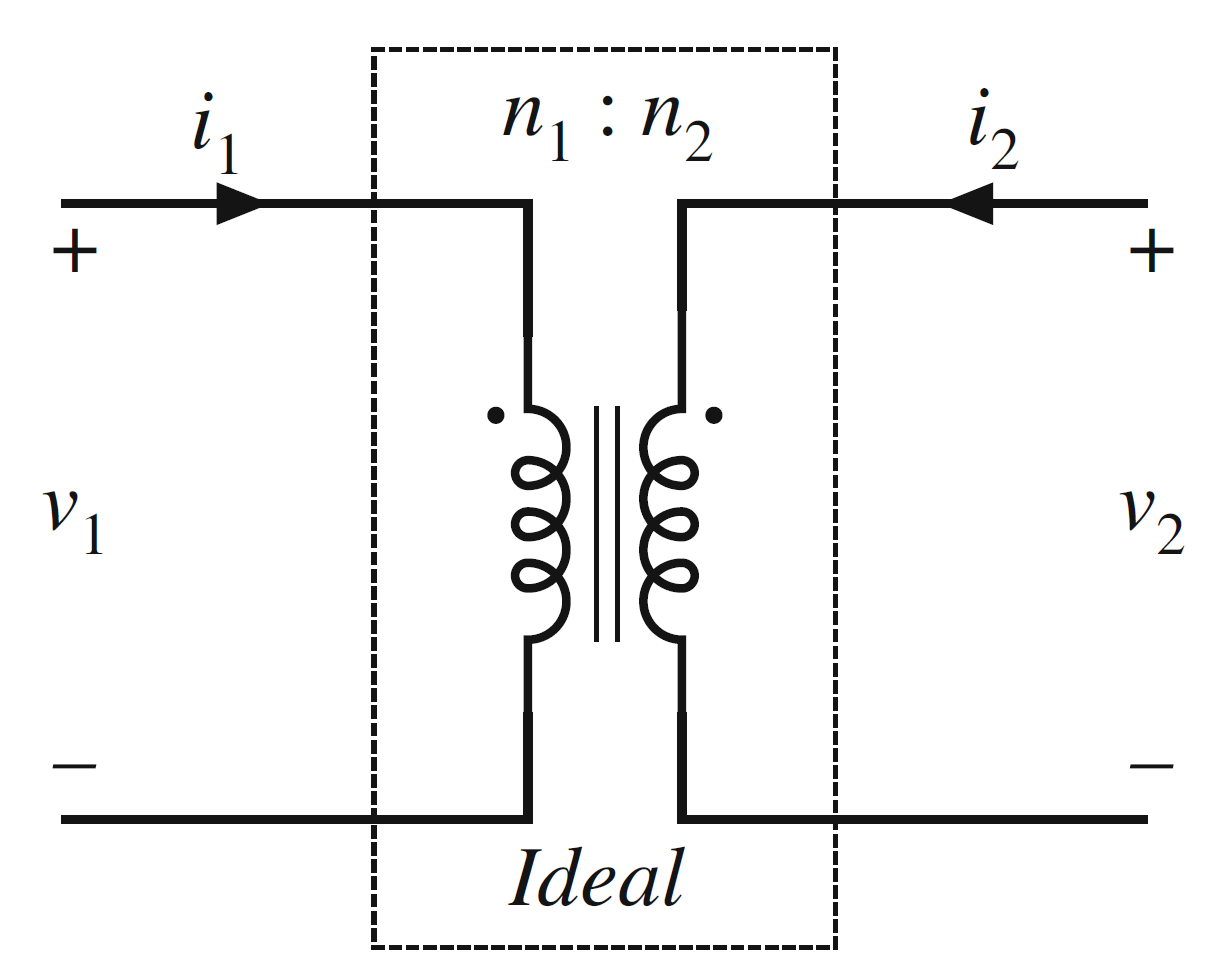
\includegraphics[width=0.7\linewidth]{fig/lec07/Ideal_Transformer_Model.png}
                \caption{Ideal transformer representation. Adapted from Erickson and Maksimovic, \textit{Fundamentals of Power Electronics}, 3rd edition, Springer, 2013.}
            \end{figure}
        \end{column}
    \end{columns}
\end{frame}


%%%%%%%%%%%%%%%%%%%%%%%%%%%%%%%%%%%%%%%%%%%%%%%%%%%%%%%%%%%%%
%% Voltage ratio
%%%%%%%%%%%%%%%%%%%%%%%%%%%%%%%%%%%%%%%%%%%%%%%%%%%%%%%%%%%%%
\begin{frame}
    \frametitle{Voltage Transformation Ratio}
    \begin{columns}
        \begin{column}{0.58\textwidth}
            Applying Faraday's law to both windings,
            \begin{align}
                v_1 &= N_1\frac{d\Phi}{dt}
            \end{align}
            \begin{align}
                v_2 &= N_2\frac{d\Phi}{dt}
            \end{align}
            Dividing the equations gives
            \begin{align}
                \frac{v_2}{v_1} &= \frac{N_2}{N_1}
            \end{align}
        \end{column}
        \begin{column}{0.38\textwidth}
            This relation determines whether the transformer acts as:
            \begin{itemize}
                \item Step-up transformer
                \item Step-down transformer
                \item Isolation transformer
            \end{itemize}
            \begin{block}{Example}
                $N_1=20$ and $N_2=100$
                \begin{equation}
                    \frac{V_2}{V_1}=5
                \end{equation}
                Voltage is increased by a factor of five.
            \end{block}
        \end{column}
    \end{columns}
\end{frame}


%%%%%%%%%%%%%%%%%%%%%%%%%%%%%%%%%%%%%%%%%%%%%%%%%%%%%%%%%%%%%
%% Current ratio
%%%%%%%%%%%%%%%%%%%%%%%%%%%%%%%%%%%%%%%%%%%%%%%%%%%%%%%%%%%%%
\begin{frame}
    \frametitle{Current Transformation Ratio}
    \begin{columns}
        \begin{column}{0.45\textwidth}
            Power conservation in an ideal transformer requires
            \begin{align}
                v_1 i_1 &= v_2 i_2
            \end{align}
            Using
            \begin{align}
                \frac{v_2}{v_1} &= \frac{N_2}{N_1}
            \end{align}
            gives
            \begin{align}
                \frac{i_2}{i_1} &= \frac{N_1}{N_2}
            \end{align}
        \end{column}
        \begin{column}{0.5\textwidth}
            \begin{block}{Design Insight}
                High-voltage winding $\Rightarrow$ low current \\
                Low-voltage winding $\Rightarrow$ high current
            \end{block}
            Important observations:
            \begin{itemize}
                \item Voltage increases with turns ratio.
                \item Current decreases with turns ratio.
                \item Power remains unchanged in the ideal case.
            \end{itemize}
        \end{column}
    \end{columns}
\end{frame}


%%%%%%%%%%%%%%%%%%%%%%%%%%%%%%%%%%%%%%%%%%%%%%%%%%%%%%%%%%%%%
%% Ampere turn balance
%%%%%%%%%%%%%%%%%%%%%%%%%%%%%%%%%%%%%%%%%%%%%%%%%%%%%%%%%%%%%
\begin{frame}
    \frametitle{Ampere-Turn Balance}
    \begin{columns}
        \begin{column}{0.58\textwidth}
            Applying Amp\`ere's law around the magnetic core yields
            \begin{align}
                N_1 i_1 + N_2 i_2 &= 0
            \end{align}
            This relation is called ampere-turn balance.
            \vspace{0.15cm}
            Physically:
            \begin{itemize}
                \item Primary current establishes flux.
                \item Secondary current opposes that flux.
                \item The core adjusts so that net flux remains finite.
            \end{itemize}
            \vspace{0.15cm}
            This is the magnetic equivalent of current balance in electrical circuits.
        \end{column}
        \begin{column}{0.38\textwidth}
            \begin{block}{Key Result}
                \begin{align}
                    N_1 i_1 &= -N_2 i_2
                \end{align}
                Ampere-turns cancel.
            \end{block}
        \end{column}
    \end{columns}
\end{frame}


%%%%%%%%%%%%%%%%%%%%%%%%%%%%%%%%%%%%%%%%%%%%%%%%%%%%%%%%%%%%%
%% Magnetizing current
%%%%%%%%%%%%%%%%%%%%%%%%%%%%%%%%%%%%%%%%%%%%%%%%%%%%%%%%%%%%%
\begin{frame}
    \frametitle{Magnetizing Current}
    \begin{columns}
        \begin{column}{0.58\textwidth}
            A practical transformer requires a finite current to establish magnetic flux. This current is called the magnetizing current. Using
            $L_m = \frac{N^2}{\mathcal R}$ the magnetizing current becomes
            \begin{align}
                i_m &= \frac{1}{L_m} \int v\,dt
            \end{align}
            \vspace{0.15cm}
            Magnetizing current:
            \begin{itemize}
                \item Exists even under no-load conditions.
                \item Establishes the required core flux.
                \item Is usually much smaller than load current.
            \end{itemize}
        \end{column}
        \begin{column}{0.38\textwidth}
            \begin{figure}
                \centering
                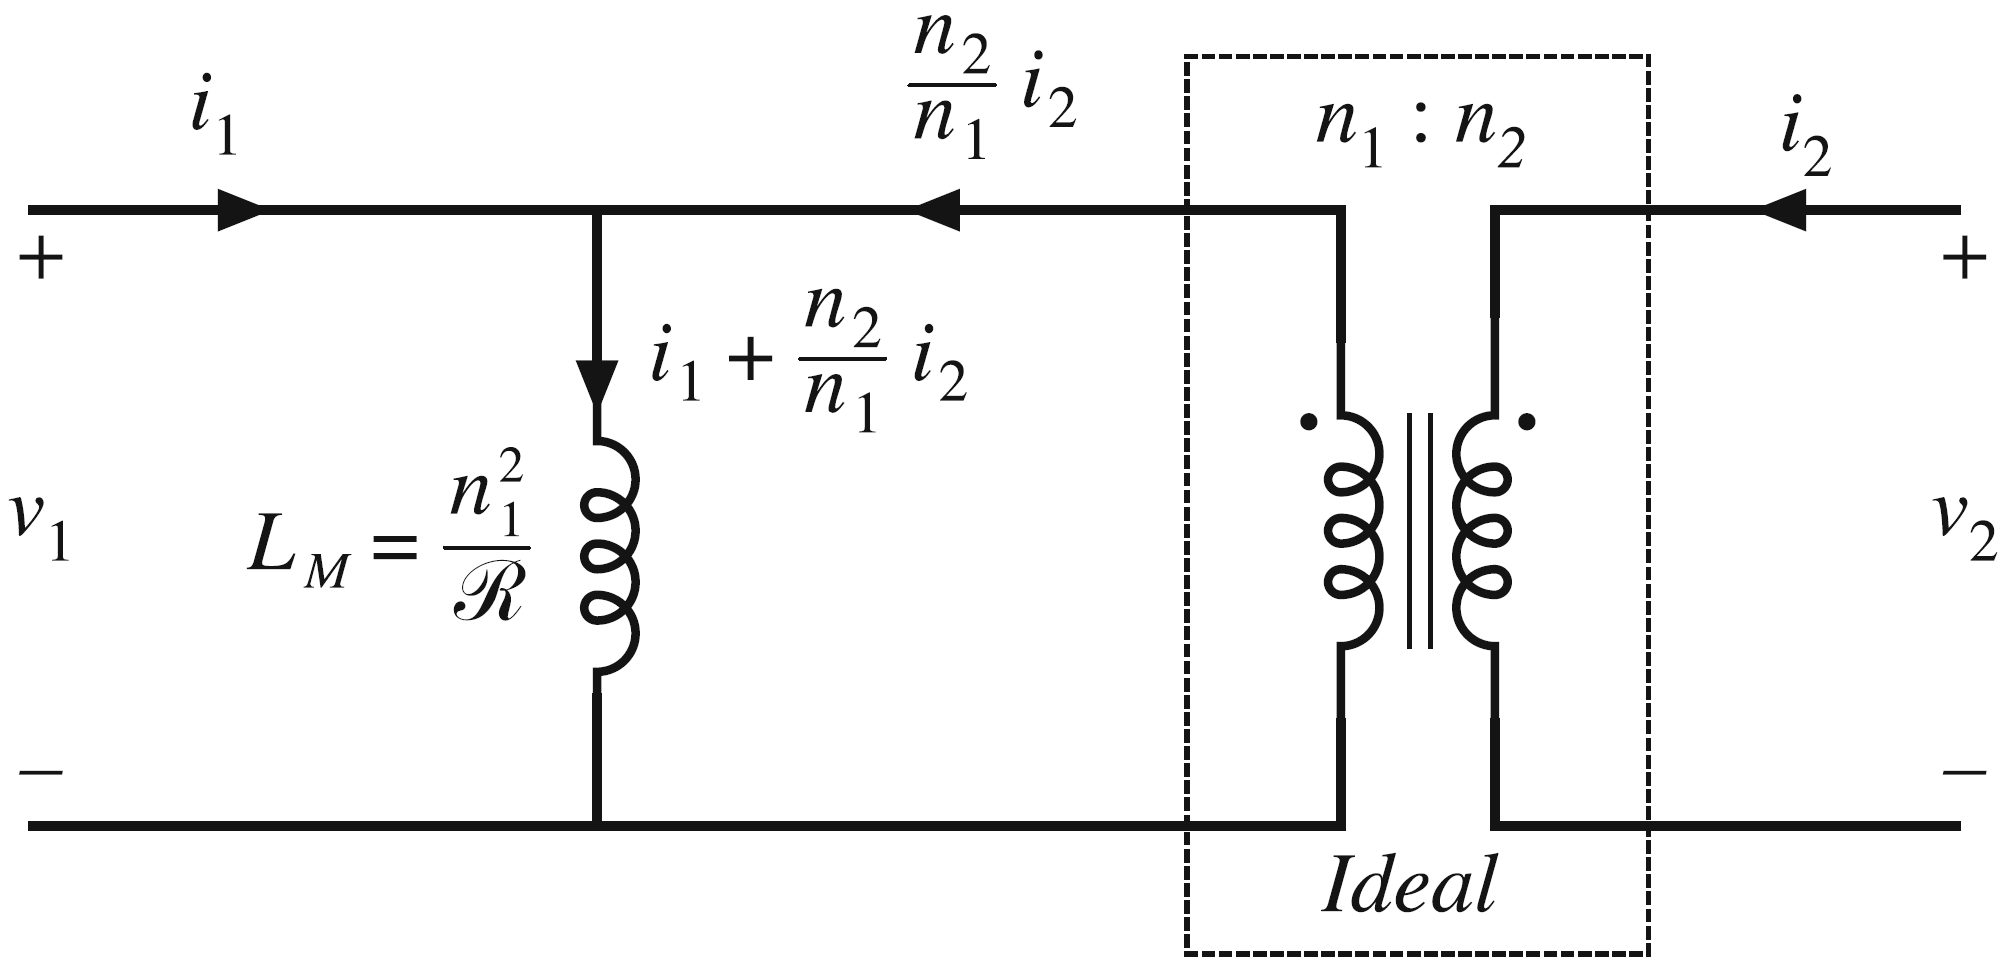
\includegraphics[width=\linewidth]{fig/lec07/Magnetizing_Inductance.png}
                \caption{Magnetizing inductance representation in a practical transformer. Adapted from Erickson and Maksimovic, \textit{Fundamentals of Power Electronics}, 3rd edition, Springer, 2013.}
            \end{figure}
        \end{column}
    \end{columns}
\end{frame}


%%%%%%%%%%%%%%%%%%%%%%%%%%%%%%%%%%%%%%%%%%%%%%%%%%%%%%%%%%%%%
%% Magnetizing inductance
%%%%%%%%%%%%%%%%%%%%%%%%%%%%%%%%%%%%%%%%%%%%%%%%%%%%%%%%%%%%%
\begin{frame}
    \frametitle{Physical Meaning of Magnetizing Inductance}
    \begin{columns}
        \begin{column}{0.58\textwidth}
            Magnetizing inductance represents the ability of the transformer core to establish magnetic flux.
            \vspace{0.15cm}
            \begin{align}
                L_m &= \frac{N^2}{\mathcal R}
            \end{align}
            Therefore,
            \begin{itemize}
                \item Higher permeability increases $L_m$.
                \item More turns increase $L_m$.
                \item Air gaps reduce $L_m$.
                \item Lower reluctance increases $L_m$.
            \end{itemize}
            \vspace{0.15cm}
            Power transformers generally seek a large magnetizing inductance to minimize no-load current.
        \end{column}
        \begin{column}{0.38\textwidth}
            \begin{block}{Transformer Design Goal}
                Large
                \begin{equation}
                    L_m
                \end{equation}
                \vspace{0.15cm}
                Small
                \begin{equation}
                    i_m
                \end{equation}
                \vspace{0.15cm}
                High efficiency
            \end{block}
        \end{column}
    \end{columns}
\end{frame}


%%%%%%%%%%%%%%%%%%%%%%%%%%%%%%%%%%%%%%%%%%%%%%%%%%%%%%%%%%%%%
%% Practical transformer
%%%%%%%%%%%%%%%%%%%%%%%%%%%%%%%%%%%%%%%%%%%%%%%%%%%%%%%%%%%%%
\begin{frame}
    \frametitle{Practical Transformer Equivalent Circuit}
    \begin{columns}
        \begin{column}{0.58\textwidth}
            Real transformers deviate from the ideal model because of:
            \begin{itemize}
                \item Copper resistance
                \item Leakage inductance
                \item Core loss
                \item Finite permeability
            \end{itemize}
            \vspace{0.15cm}
            The practical transformer therefore includes:
            \begin{itemize}
                \item Winding resistances
                \item Magnetizing inductance
                \item Core-loss resistance
                \item Leakage inductances
            \end{itemize}
            \vspace{0.15cm}
        \end{column}
        \begin{column}{0.38\textwidth}
            \begin{figure}
                \centering
                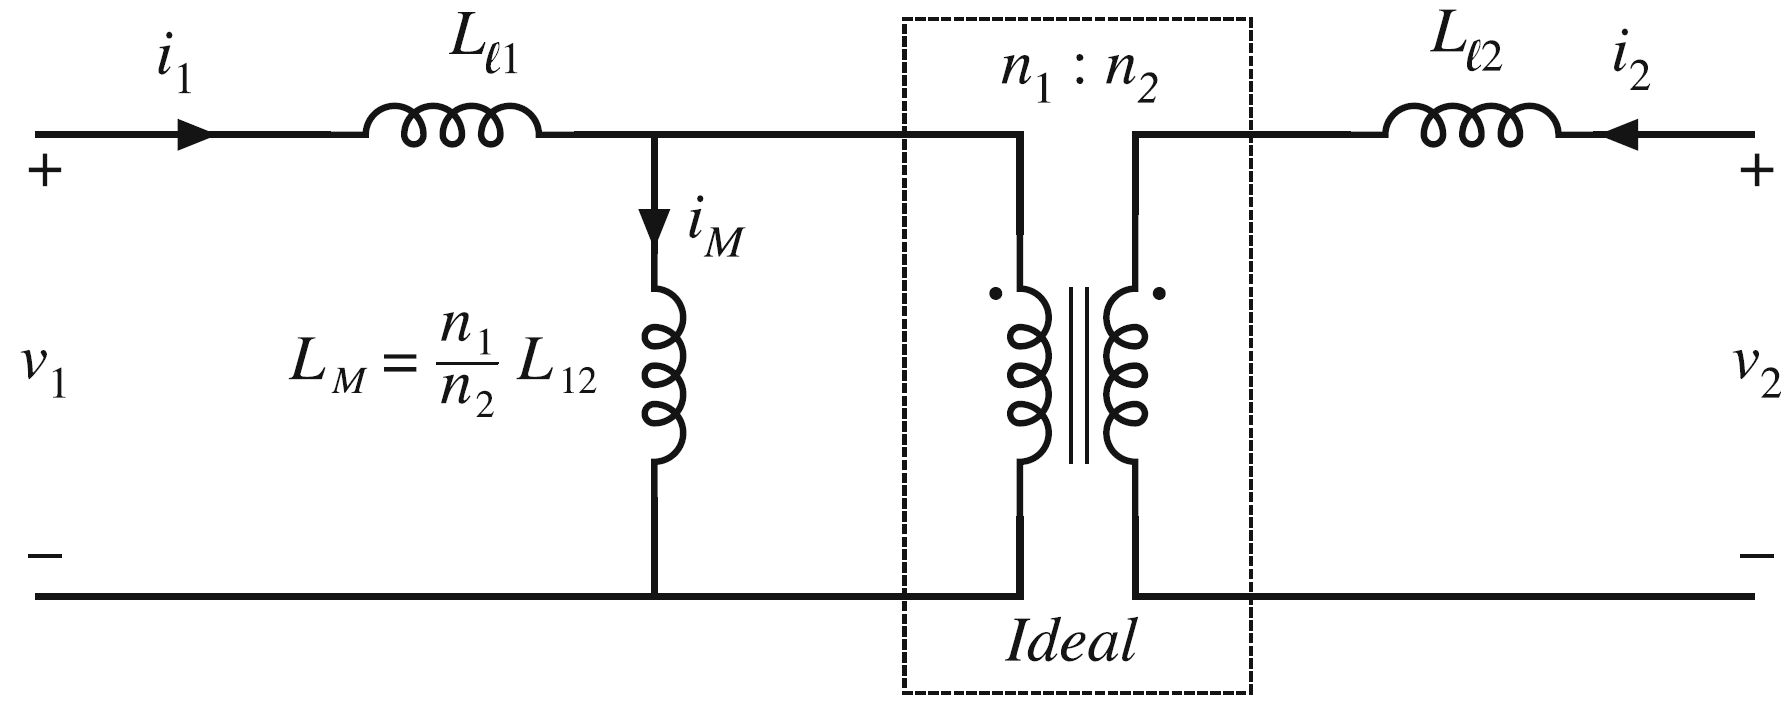
\includegraphics[width=\linewidth]{fig/lec07/Practical_Transformer_Equivalent.png}
                \caption{Practical transformer equivalent circuit including magnetizing branch and parasitic elements. Adapted from Erickson and Maksimovic, \textit{Fundamentals of Power Electronics}, 3rd edition, Springer, 2013.}
            \end{figure}
            This equivalent circuit is extensively used in transformer design and simulation.
        \end{column}
    \end{columns}
\end{frame}



% Next I should prepare slides on design of transformers including current transformers, then I want to talk about the losses, then I want to talk about the new versions like planer magnetics, MHz magnetics, and then I want to talk about the design of magnetic components for high frequency applications. Also, if possible something in direction of winding arrangements and cooling. This will conclude the magnetics. 


%%%%%%%%%%%%%%%%%%%%%%%%%%%%%%%%%%%%%%%%%%%%%%%%%%%%%%%%%%%%%
%% Practical magnetic components
%%%%%%%%%%%%%%%%%%%%%%%%%%%%%%%%%%%%%%%%%%%%%%%%%%%%%%%%%%%%%
\begin{frame}
\begin{center}
  \textbf{\Huge{Practical Magnetic Components}}\\[0.4cm]
  \textbf{\Large{Inductors, Transformers, Coupled Inductors, and Current Transformers}}
\end{center}
\end{frame}


%%%%%%%%%%%%%%%%%%%%%%%%%%%%%%%%%%%%%%%%%%%%%%%%%%%%%%%%%%%%%
%% Magnetic component families
%%%%%%%%%%%%%%%%%%%%%%%%%%%%%%%%%%%%%%%%%%%%%%%%%%%%%%%%%%%%%
\begin{frame}
    \frametitle{Main Families of Magnetic Components in Power Electronics}
    \begin{columns}
        \begin{column}{0.58\textwidth}
            Magnetic components in power electronics can be grouped according to their dominant function.

            \vspace{0.15cm}

            \begin{itemize}
                \item \textbf{Energy-storage components}
                \begin{itemize}
                    \item DC filter inductors
                    \item AC inductors or line reactors
                    \item Flyback magnetic components
                \end{itemize}

                \item \textbf{Energy-transfer components}
                \begin{itemize}
                    \item High-frequency transformers
                    \item Pulse transformers
                    \item Current transformers
                \end{itemize}

                \item \textbf{Coupled and integrated components}
                \begin{itemize}
                    \item Coupled inductors
                    \item Integrated magnetics
                    \item Planar magnetics
                \end{itemize}
            \end{itemize}
        \end{column}

        \begin{column}{0.38\textwidth}
            The correct magnetic component is selected from converter function, isolation requirement, stored energy, frequency, current ripple, and thermal constraints.
            \begin{block}{Key Design Question}
                Is the component mainly required to store energy, transfer energy, sense current, or combine several magnetic functions?
            \end{block}
        \end{column}
    \end{columns}
\end{frame}


%%%%%%%%%%%%%%%%%%%%%%%%%%%%%%%%%%%%%%%%%%%%%%%%%%%%%%%%%%%%%
%% Filter inductor
%%%%%%%%%%%%%%%%%%%%%%%%%%%%%%%%%%%%%%%%%%%%%%%%%%%%%%%%%%%%%
\begin{frame}
    \frametitle{Filter Inductor}

    \begin{columns}
        \begin{column}{0.58\textwidth}
            A filter inductor is used to control current ripple and shape the current waveform in a switching converter. Typical applications include:
            \begin{itemize}
                \item Buck converter output filter
                \item Boost converter input inductor
                \item PFC boost inductor
                \item DC-link filtering
                \item EMI and differential-mode filtering
            \end{itemize}
            The governing relation is
            \begin{align}
                v_L = L\frac{di_L}{dt}
            \end{align}
            A larger inductance reduces ripple, but also increases volume, copper loss, and stored energy requirement.
        \end{column}

        \begin{column}{0.38\textwidth}
            \begin{block}{Design Focus}
                \small
                For a filter inductor, the most important quantities are:
                \begin{itemize}
                    \item Required inductance $L$
                    \item Peak current $I_{\mathrm{pk}}$
                    \item RMS current $I_{\mathrm{rms}}$
                    \item Allowed ripple $\Delta i$
                    \item Saturation current
                    \item Temperature rise
                \end{itemize}
            \end{block}
        \end{column}
    \end{columns}
\end{frame}


%%%%%%%%%%%%%%%%%%%%%%%%%%%%%%%%%%%%%%%%%%%%%%%%%%%%%%%%%%%%%
%% AC inductor
%%%%%%%%%%%%%%%%%%%%%%%%%%%%%%%%%%%%%%%%%%%%%%%%%%%%%%%%%%%%%
\begin{frame}
    \frametitle{AC Inductor or Line Reactor}
    \begin{columns}
        \begin{column}{0.58\textwidth}
            An AC inductor, often called a line reactor, is used when the current is alternating rather than purely DC with ripple. It is commonly used in:
            \begin{itemize}
                \item Grid-connected converters
                \item Three-phase rectifiers
                \item Motor-drive output filters
                \item Active front-end converters
                \item LCL filters for inverters
            \end{itemize}
            Unlike a DC filter inductor, an AC inductor experiences bidirectional flux swing. So, the design must consider:
            \begin{itemize}
                \item Fundamental-frequency current
                \item Switching-frequency ripple
                \item Core loss under AC excitation
                \item Audible noise and vibration
            \end{itemize}
        \end{column}

        \begin{column}{0.38\textwidth}
            \begin{block}{Practical Difference}
                A DC filter inductor is often limited by peak current and saturation. An AC inductor is often limited by combined copper loss, core loss, thermal rise, and insulation stress.
            \end{block}
        \end{column}
    \end{columns}
\end{frame}


%%%%%%%%%%%%%%%%%%%%%%%%%%%%%%%%%%%%%%%%%%%%%%%%%%%%%%%%%%%%%
%% Coupled inductor
%%%%%%%%%%%%%%%%%%%%%%%%%%%%%%%%%%%%%%%%%%%%%%%%%%%%%%%%%%%%%
\begin{frame}
    \frametitle{Coupled Inductor}

    \begin{columns}
        \begin{column}{0.58\textwidth}
            A coupled inductor contains two or more windings on a common magnetic core. The windings share part of their magnetic flux. The coupling is described by the mutual inductance $M$ and the coupling coefficient $k$:
            \begin{align}
                k = \frac{M}{\sqrt{L_1L_2}}, \qquad 0 \leq k \leq 1
            \end{align}
            Coupled inductors are useful in:
            \begin{itemize}
                \item Interleaved buck converters
                \item Multiphase voltage regulators
                \item Coupled-inductor boost converters
                \item Ripple-current cancellation
                \item Integrated magnetic structures
            \end{itemize}

        \end{column}

        \begin{column}{0.38\textwidth}
            \begin{figure}
                \centering
                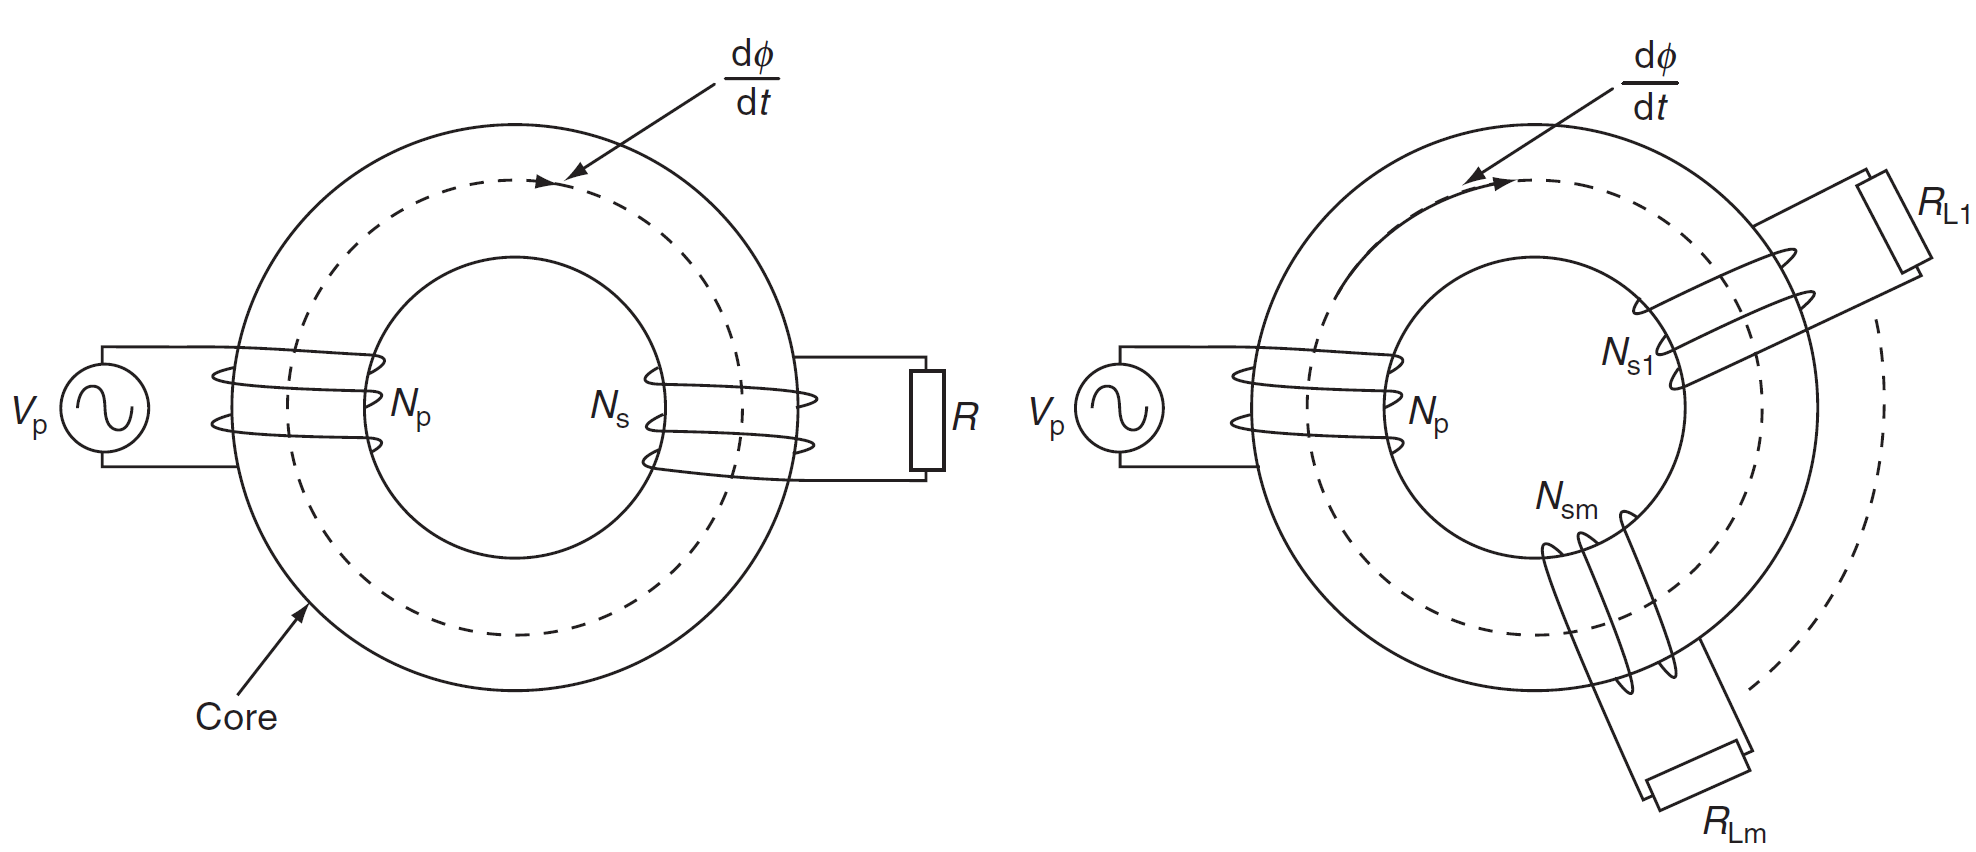
\includegraphics[width=\linewidth]{fig/lec07/coupled_inductor_ill.png}
                \caption{Multiple-winding magnetic structure illustrating shared magnetic coupling. Adapted from Umanand, \textit{Power Electronics: Essentials and Applications}}
            \end{figure}
        \end{column}
    \end{columns}
\end{frame}

%%%%%%%%%%%%%%%%%%%%%%%%%%%%%%%%%%%%%%%%%%%%%%%%%%%%%%%%%%%%%
%% Coupled inductor
%%%%%%%%%%%%%%%%%%%%%%%%%%%%%%%%%%%%%%%%%%%%%%%%%%%%%%%%%%%%%
\begin{frame}
    \frametitle{Coupled Inductor}

    \begin{columns}
        \begin{column}{0.58\textwidth}
            As in the case of the single winding filter inductor, the size of the minor B-H loop is proportional to the total current ripple (Fig. 10.48). Small ripple implies small core loss, as well as small proximity loss. An air gap is employed, and the maximum flux density is typically limited by saturation.
        \end{column}

        \begin{column}{0.38\textwidth}
            \begin{figure}
                \centering
                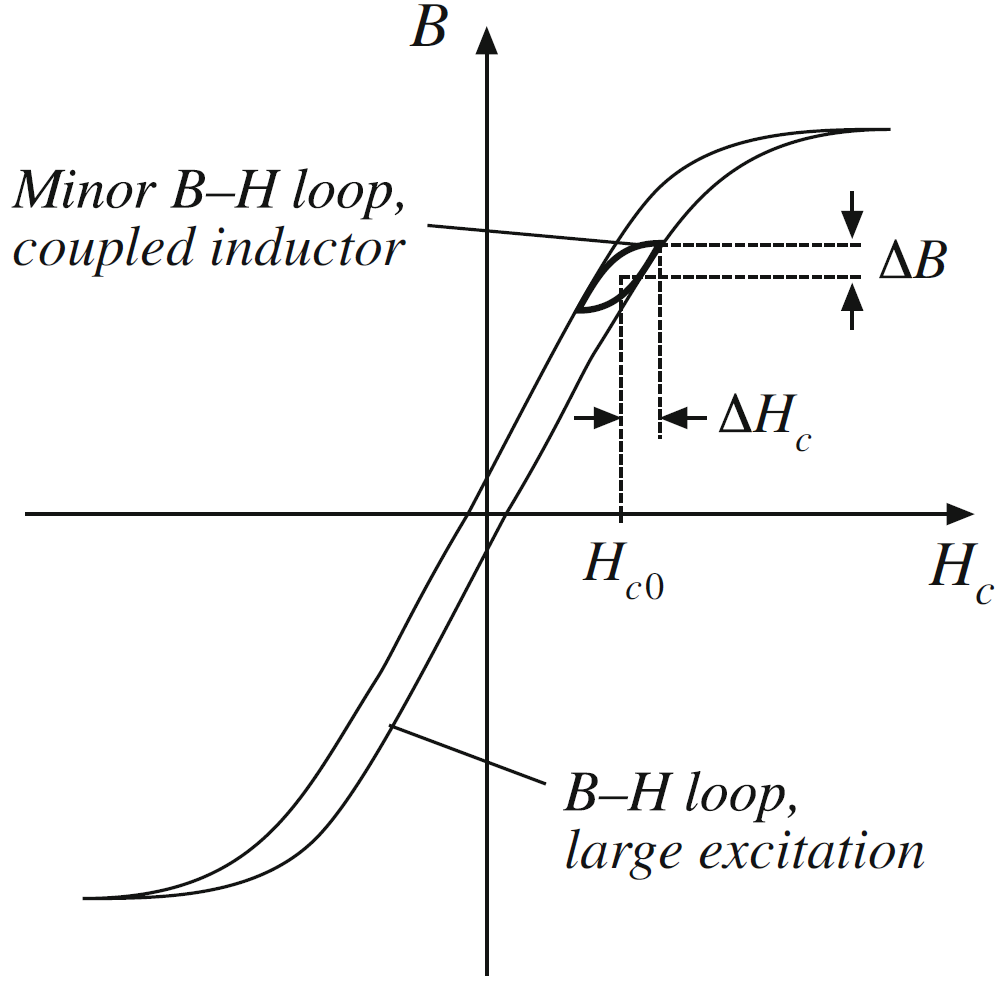
\includegraphics[width=0.8\linewidth]{fig/lec07/coupled_inductor.png}
                \caption{Coupled inductor minor B-H loop. Adapted from Errikson and Maksimovic, \textit{Fundamentals of Power Electronics}, 3rd edition, Springer, 2013}
            \end{figure}
        \end{column}
    \end{columns}
\end{frame}


%%%%%%%%%%%%%%%%%%%%%%%%%%%%%%%%%%%%%%%%%%%%%%%%%%%%%%%%%%%%%
%% True transformer
%%%%%%%%%%%%%%%%%%%%%%%%%%%%%%%%%%%%%%%%%%%%%%%%%%%%%%%%%%%%%
\begin{frame}
    \frametitle{High-Frequency Transformer}
    \begin{columns}
        \begin{column}{0.58\textwidth}
            A high-frequency transformer transfers energy between two or more electrical ports through a shared magnetic flux. It is used for:
            \begin{itemize}
                \item Galvanic isolation
                \item Voltage step-up or step-down
                \item Impedance matching
                \item Multiple isolated outputs
            \end{itemize}
            Applying Faraday's law to two windings gives
            \begin{align}
                \frac{v_1}{N_1} = \frac{v_2}{N_2}
            \end{align}

            and ideal ampere-turn balance gives

            \begin{align}
                N_1 i_1 + N_2 i_2 = 0
            \end{align}
        \end{column}

        \begin{column}{0.38\textwidth}
            A true transformer should ideally transfer energy, not store significant energy.
            \begin{figure}
                \centering
                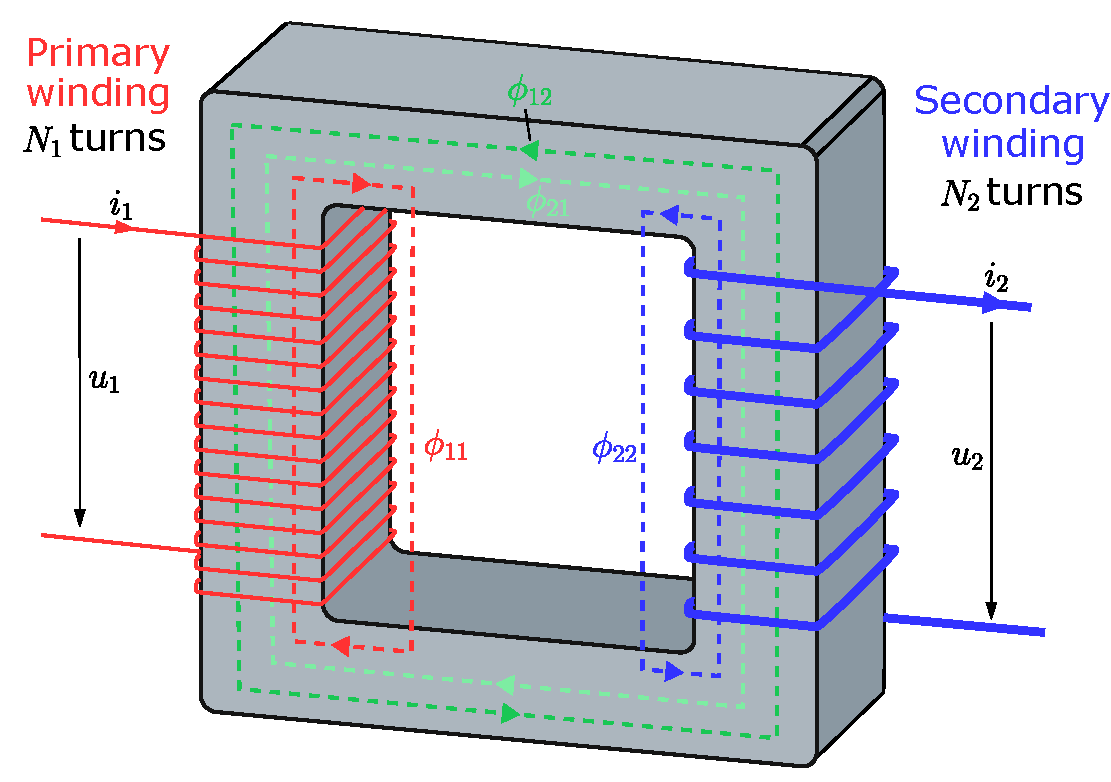
\includegraphics[width=\linewidth]{fig/lec07/Transformer3d_col3.pdf}
                \caption{Operating principle of a transformer with primary and secondary windings linked by common flux.}
            \end{figure}
        \end{column}
    \end{columns}
\end{frame}


%%%%%%%%%%%%%%%%%%%%%%%%%%%%%%%%%%%%%%%%%%%%%%%%%%%%%%%%%%%%%
%% Flyback transformer
%%%%%%%%%%%%%%%%%%%%%%%%%%%%%%%%%%%%%%%%%%%%%%%%%%%%%%%%%%%%%
\begin{frame}
    \frametitle{Flyback Transformer: Actually a Coupled Inductor}
    \begin{columns}
        \begin{column}{0.58\textwidth}
            The term ``flyback transformer'' is widely used in industry, but magnetically it is more accurately a coupled inductor. In a true transformer:
            \begin{itemize}
                \item Primary and secondary currents flow simultaneously.
                \item Ampere-turns largely cancel.
                \item Energy storage is undesirable.
            \end{itemize}
            In a flyback magnetic component:
            \begin{itemize}
                \item Primary and secondary currents occur sequentially.
                \item Energy is first stored in magnetizing inductance.
                \item Energy is later delivered to the secondary.
                \item An air gap is essential for energy storage.
            \end{itemize}
            \begin{align}
                E = \frac{1}{2}L_m I_{\mathrm{pk}}^2
            \end{align}
        \end{column}
        \begin{column}{0.38\textwidth}
            \vspace{-1cm}
            \begin{figure}
                \centering
                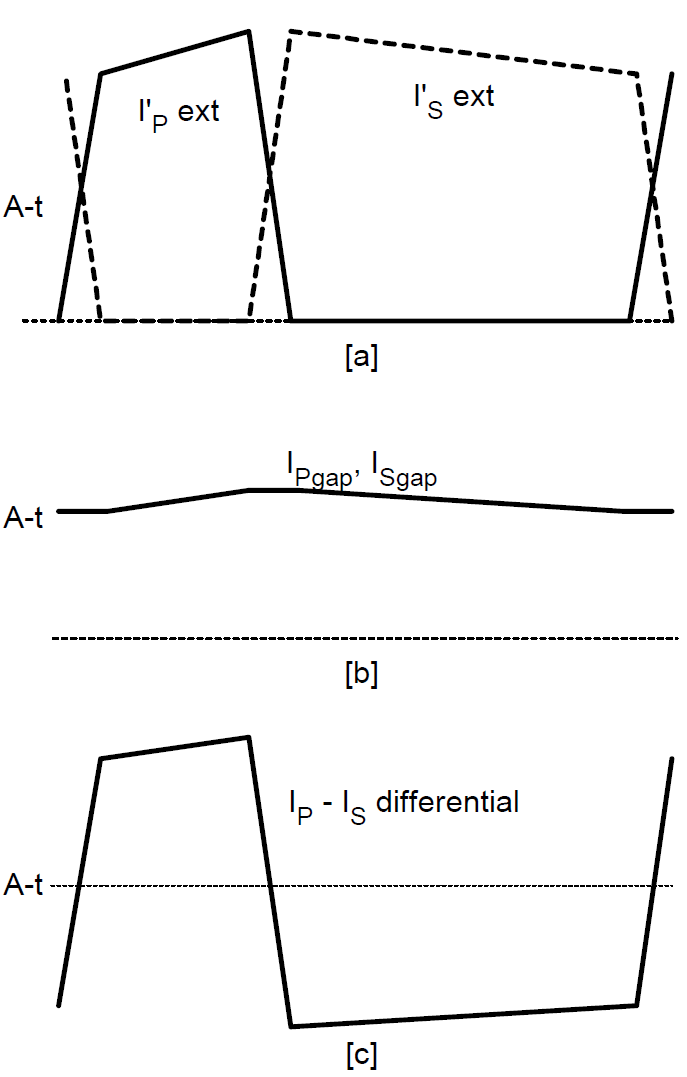
\includegraphics[width=0.6\linewidth]{fig/lec07/flyback_inductor.png}
                \caption{Continuous-mode flyback winding ampere-turn waveforms showing sequential primary and secondary current action. Adapted from Dixon, Texas Instruments, \textit{Designing Planar Magnetics}}
            \end{figure}
        \end{column}
    \end{columns}
\end{frame}


%%%%%%%%%%%%%%%%%%%%%%%%%%%%%%%%%%%%%%%%%%%%%%%%%%%%%%%%%%%%%
%% Current transformer
%%%%%%%%%%%%%%%%%%%%%%%%%%%%%%%%%%%%%%%%%%%%%%%%%%%%%%%%%%%%%
\begin{frame}
    \frametitle{Current Transformer}
    \begin{columns}
        \begin{column}{0.58\textwidth}
            A current transformer is a magnetic sensor used to reproduce a scaled version of a primary current in an isolated secondary circuit. For an ideal current transformer,
            \begin{align}
                \frac{I_s}{I_p} \approx \frac{N_p}{N_s}
            \end{align}
            Typical uses include:
            \begin{itemize}
                \item Isolated current sensing
                \item Over-current protection
                \item Gate-drive power sensing
                \item Converter diagnostics
                \item Protection relays
            \end{itemize}

        \end{column}
        \begin{column}{0.38\textwidth}
            The secondary current is usually converted to a voltage using a burden resistor:
            \begin{align}
                v_s = I_s R_b
            \end{align}
            \vspace{-0.75cm}
            \begin{block}{Safety Note}
                \small
                A current-transformer secondary should not be open-circuited while primary current is flowing. A large voltage can be induced across the secondary winding.
            \end{block}
            \begin{block}{Design Focus}
                \small
                Important parameters are turns ratio, burden resistance, saturation current, bandwidth, leakage inductance, and insulation rating.
            \end{block}
        \end{column}
    \end{columns}
\end{frame}


%%%%%%%%%%%%%%%%%%%%%%%%%%%%%%%%%%%%%%%%%%%%%%%%%%%%%%%%%%%%%
%% Leakage flux in transformers
%%%%%%%%%%%%%%%%%%%%%%%%%%%%%%%%%%%%%%%%%%%%%%%%%%%%%%%%%%%%%
\begin{frame}
    \frametitle{Leakage Flux in Transformer-Type Magnetics}

    \begin{columns}
        \begin{column}{0.58\textwidth}
            In practical transformers, not all magnetic flux links both windings. The flux that links only one winding is called leakage flux. It appears electrically as leakage inductance.
            Leakage inductance can be harmful or useful depending on the converter:
            \begin{itemize}
                \item In hard-switched converters, it causes voltage overshoot and ringing.
                \item In isolated converters, it can slow current transfer between windings.
                \item In resonant converters such as LLC converters, it can become part of the resonant tank.
            \end{itemize}
            Therefore, leakage inductance is not simply a parasitic; it is a design variable.
        \end{column}

        \begin{column}{0.38\textwidth}
            \begin{figure}
                \centering
                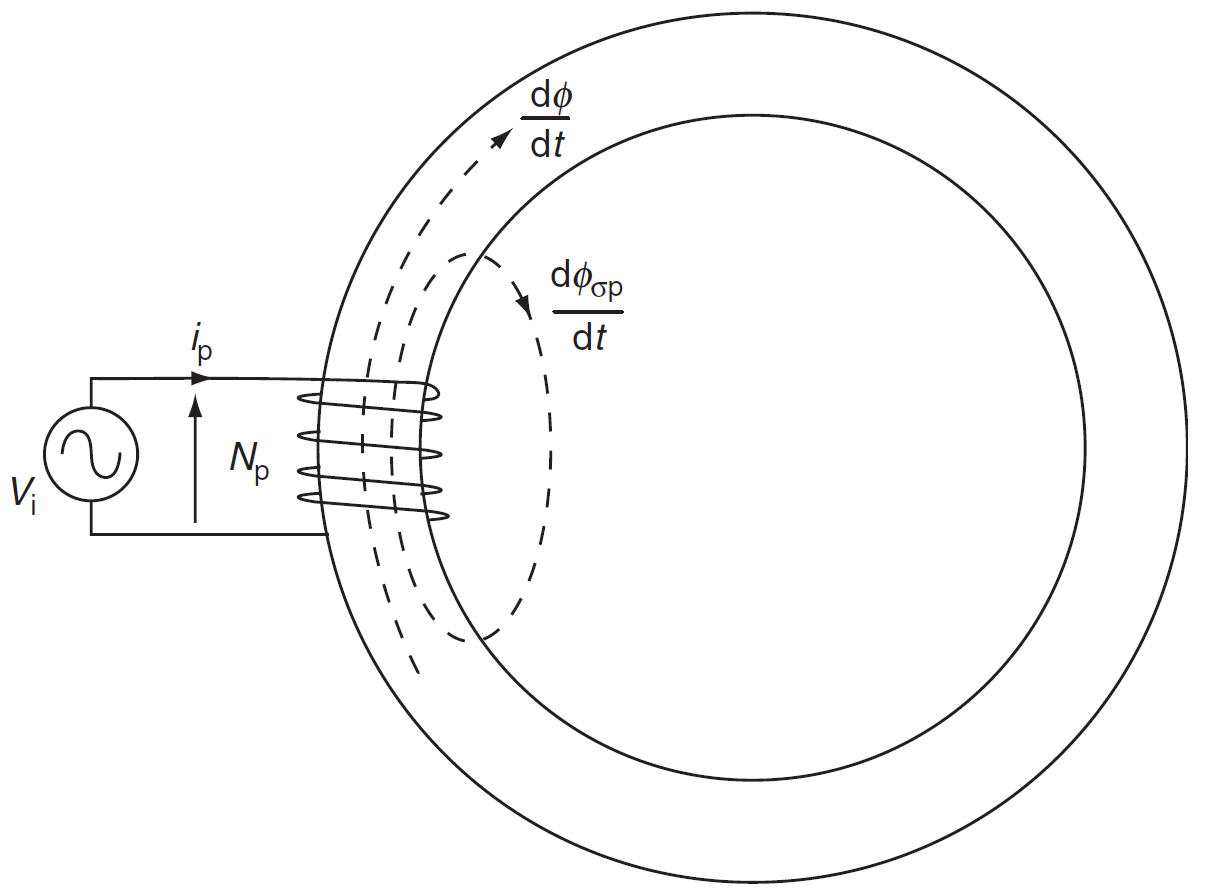
\includegraphics[width=\linewidth]{fig/lec07/linkage_flux.png}
                \caption{Leakage flux that does not fully link the second winding. Adapted from Umanand, \textit{Power Electronics: Essentials and Applications}}
            \end{figure}
        \end{column}
    \end{columns}
\end{frame}


%%%%%%%%%%%%%%%%%%%%%%%%%%%%%%%%%%%%%%%%%%%%%%%%%%%%%%%%%%%%%
%% Comparison of magnetic components
%%%%%%%%%%%%%%%%%%%%%%%%%%%%%%%%%%%%%%%%%%%%%%%%%%%%%%%%%%%%%
\begin{frame}
    \frametitle{Comparison of Practical Magnetic Components}

    \scriptsize
    \begin{table}
        \centering
        \begin{tabular}{p{0.22\textwidth}p{0.15\textwidth}p{0.15\textwidth}p{0.13\textwidth}p{0.22\textwidth}}
            \hline
            \textbf{Component} & \textbf{Stores Energy} & \textbf{Transfers Energy} & \textbf{Air Gap} & \textbf{Typical Use}\\
            \hline
            Filter inductor & Yes & No & Usually yes & Buck, boost, PFC, DC filters\\
            AC inductor / reactor & Yes & No & Sometimes & Grid filters, motor drives, rectifiers\\
            Coupled inductor & Yes & Partly & Sometimes & Interleaved converters, ripple cancellation\\
            Flyback transformer & Yes & Sequentially & Yes & Isolated low/medium-power supplies\\
            HF transformer & Ideally no & Yes & Usually no & LLC, DAB, PSFB, isolated converters\\
            Current transformer & No & Signal energy only & No & Sensing and protection\\
            \hline
        \end{tabular}
    \end{table}
    \begin{block}{Message}
        \small
        The distinction between stored energy and transferred energy is the most important conceptual difference between inductors, flyback magnetic components, and true transformers.
    \end{block}
\end{frame}

%%%%%%%%%%%%%%%%%%%%%%%%%%%%%%%%%%%%%%%%%%%%%%%%%%%%%%%%%%%%%
%% Transformer design section
%%%%%%%%%%%%%%%%%%%%%%%%%%%%%%%%%%%%%%%%%%%%%%%%%%%%%%%%%%%%%
\begin{frame}
\begin{center}
  \textbf{\Huge{Transformer Design}}\\[0.4cm]
  \textbf{\Large{From Converter Specification to Magnetic Hardware}}
\end{center}
\end{frame}


%%%%%%%%%%%%%%%%%%%%%%%%%%%%%%%%%%%%%%%%%%%%%%%%%%%%%%%%%%%%%
%% Transformer design inputs
%%%%%%%%%%%%%%%%%%%%%%%%%%%%%%%%%%%%%%%%%%%%%%%%%%%%%%%%%%%%%
\begin{frame}
    \frametitle{Transformer Design Inputs}

    \begin{columns}
        \begin{column}{0.58\textwidth}
            Transformer design begins from the converter-level specification, not from the core catalogue.

            \vspace{0.15cm}

            The main electrical inputs are:
            \begin{itemize}
                \item Input-voltage range: $V_{\mathrm{in,min}}$ to $V_{\mathrm{in,max}}$
                \item Output voltage and power: $V_o$, $P_o$
                \item Switching frequency: $f_s$
                \item Topology: flyback, forward, LLC, PSFB, DAB, etc.
                \item Maximum duty ratio or phase-shift range
                \item Required isolation voltage
                \item Allowed temperature rise
            \end{itemize}

            \vspace{0.15cm}

            These specifications determine the required volt-seconds, turns ratio, core size, winding current, insulation system, and thermal design.
        \end{column}

        \begin{column}{0.38\textwidth}
            \begin{block}{Design Message}
                \small
                A transformer cannot be designed independently of the converter topology. The applied voltage waveform determines the flux swing, while the winding currents determine copper loss and heating.
            \end{block}
        \end{column}
    \end{columns}
\end{frame}


%%%%%%%%%%%%%%%%%%%%%%%%%%%%%%%%%%%%%%%%%%%%%%%%%%%%%%%%%%%%%
%% Transformer design workflow
%%%%%%%%%%%%%%%%%%%%%%%%%%%%%%%%%%%%%%%%%%%%%%%%%%%%%%%%%%%%%
\begin{frame}
    \frametitle{Transformer Design Workflow}

    \begin{center}
    \begin{circuitikz}[scale=0.78, transform shape]
        \tikzstyle{block} = [draw, rounded corners, align=center,
        minimum width=3.0cm, minimum height=0.85cm]

        \node[block] (spec) at (0,0) {Converter\\specification};
        \node[block] (wave) at (4,0) {Voltage/current\\waveforms};
        \node[block] (core) at (8,0) {Core material\\and geometry};

        \node[block] (turns) at (8,-2) {Turns ratio and\\primary turns};
        \node[block] (wind) at (4,-2) {Winding area,\\wire/PCB traces};
        \node[block] (loss) at (0,-2) {Core loss and\\copper loss};

        \node[block] (thermal) at (0,-4) {Thermal and\\insulation check};
        \node[block] (iterate) at (4,-4) {Iterate design};
        \node[block] (proto) at (8,-4) {Prototype and\\measure};

        \draw[->, thick] (spec) -- (wave);
        \draw[->, thick] (wave) -- (core);
        \draw[->, thick] (core) -- (turns);
        \draw[->, thick] (turns) -- (wind);
        \draw[->, thick] (wind) -- (loss);
        \draw[->, thick] (loss) -- (thermal);
        \draw[->, thick] (thermal) -- (iterate);
        \draw[->, thick] (iterate) -- (proto);
        \draw[->, thick, dashed] (iterate.north) .. controls (4,-1.0) and (6,-1.0) .. (core.south);
    \end{circuitikz}
    \end{center}

    \vspace{0.15cm}

    \begin{block}{Practical Interpretation}
        \small
        Transformer design is iterative because turns, flux density, copper area, leakage inductance, temperature rise, and insulation clearance are strongly coupled.
    \end{block}
\end{frame}


%%%%%%%%%%%%%%%%%%%%%%%%%%%%%%%%%%%%%%%%%%%%%%%%%%%%%%%%%%%%%
%% Volt-second constraint
%%%%%%%%%%%%%%%%%%%%%%%%%%%%%%%%%%%%%%%%%%%%%%%%%%%%%%%%%%%%%
\begin{frame}
    \frametitle{Volt-Second Constraint and Primary Turns}

    \begin{columns}
        \begin{column}{0.5\textwidth}
            The primary turns are selected so that the core flux density remains below the allowable limit. From Faraday's law,
            \begin{align}
                v_1(t) = N_1 A_c \frac{dB(t)}{dt}
            \end{align}
            \begin{align}
                \text{Therefore,} \quad
                \Delta B =
                \frac{1}{N_1 A_c}
                \int_{t_1}^{t_2} v_1(t)\,dt
                =
                \frac{\lambda_1}{N_1 A_c}
            \end{align}

            Rearranging gives the minimum primary turns:
            \begin{align}
                N_1 \geq
                \frac{\lambda_1}{A_c \Delta B_{\max}}
            \end{align}
        \end{column}

        \begin{column}{0.48\textwidth}
            \begin{figure}
                \centering
                \includegraphics[width=0.75\linewidth]{fig/lec07/volt_sec.png}
                \caption{$\lambda_1$ is the applied positive volt-second on the primary winding. Primary voltage waveform and applied volt-seconds $\lambda_1$ used for transformer design. Adapted from Erickson and Maksimovi\'c, \textit{Fundamentals of Power Electronics}, 3rd edition}
            \end{figure}
        \end{column}
    \end{columns}
\end{frame}


%%%%%%%%%%%%%%%%%%%%%%%%%%%%%%%%%%%%%%%%%%%%%%%%%%%%%%%%%%%%%
%% Transformer saturation
%%%%%%%%%%%%%%%%%%%%%%%%%%%%%%%%%%%%%%%%%%%%%%%%%%%%%%%%%%%%%
\begin{frame}
    \frametitle{Transformer Saturation is a Volt-Second Problem}

    \begin{columns}
        \begin{column}{0.58\textwidth}
            A transformer saturates when the applied volt-seconds force the core flux density beyond the saturation limit. The core flux density is
            \begin{align}
                B(t)=\frac{1}{N_1A_c}\int v_1(t)\,dt
            \end{align}
            Hence, transformer saturation is mainly controlled by:
            \begin{itemize}
                \item Primary voltage waveform
                \item Number of primary turns
                \item Core cross-sectional area
                \item Reset condition or volt-second balance
            \end{itemize}
            Large load current does not automatically saturate a true transformer if the primary and secondary ampere-turns cancel properly.
        \end{column}

        \begin{column}{0.38\textwidth}
            \begin{block}{Important Correction}
                \small
                Adding an air gap does not solve saturation in a conventional transformer. It mainly lowers magnetizing inductance and increases magnetizing current.
            \end{block}

            \vspace{0.15cm}

            \begin{block}{Correct Remedies}
                \small
                Increase $N_1$, increase $A_c$, reduce volt-seconds, or ensure proper core reset.
            \end{block}
        \end{column}
    \end{columns}
\end{frame}


%%%%%%%%%%%%%%%%%%%%%%%%%%%%%%%%%%%%%%%%%%%%%%%%%%%%%%%%%%%%%
%% Core geometry and material selection
%%%%%%%%%%%%%%%%%%%%%%%%%%%%%%%%%%%%%%%%%%%%%%%%%%%%%%%%%%%%%
\begin{frame}
    \frametitle{Core Geometry and Material Selection}
            Core selection determines the magnetic, electrical, thermal, and manufacturing limits of the transformer.

            \vspace{0.15cm}

            Important core parameters are:
            \begin{itemize}
                \item Effective core area $A_c$ or $A_e$
                \item Window area $A_w$ or $W_A$
                \item Magnetic path length $l_m$
                \item Mean length per turn MLT
                \item Core volume $V_c$
                \item Core material and loss data
            \end{itemize}
            Typical high-frequency core families include EE, EI, ER, ETD, PQ, RM and low-profile planar variants.
\end{frame}


\begin{frame}
    \frametitle{Core Geometry and Material Selection}
    \begin{columns}
        \begin{column}{0.5\textwidth}
            \begin{figure}
                \centering
                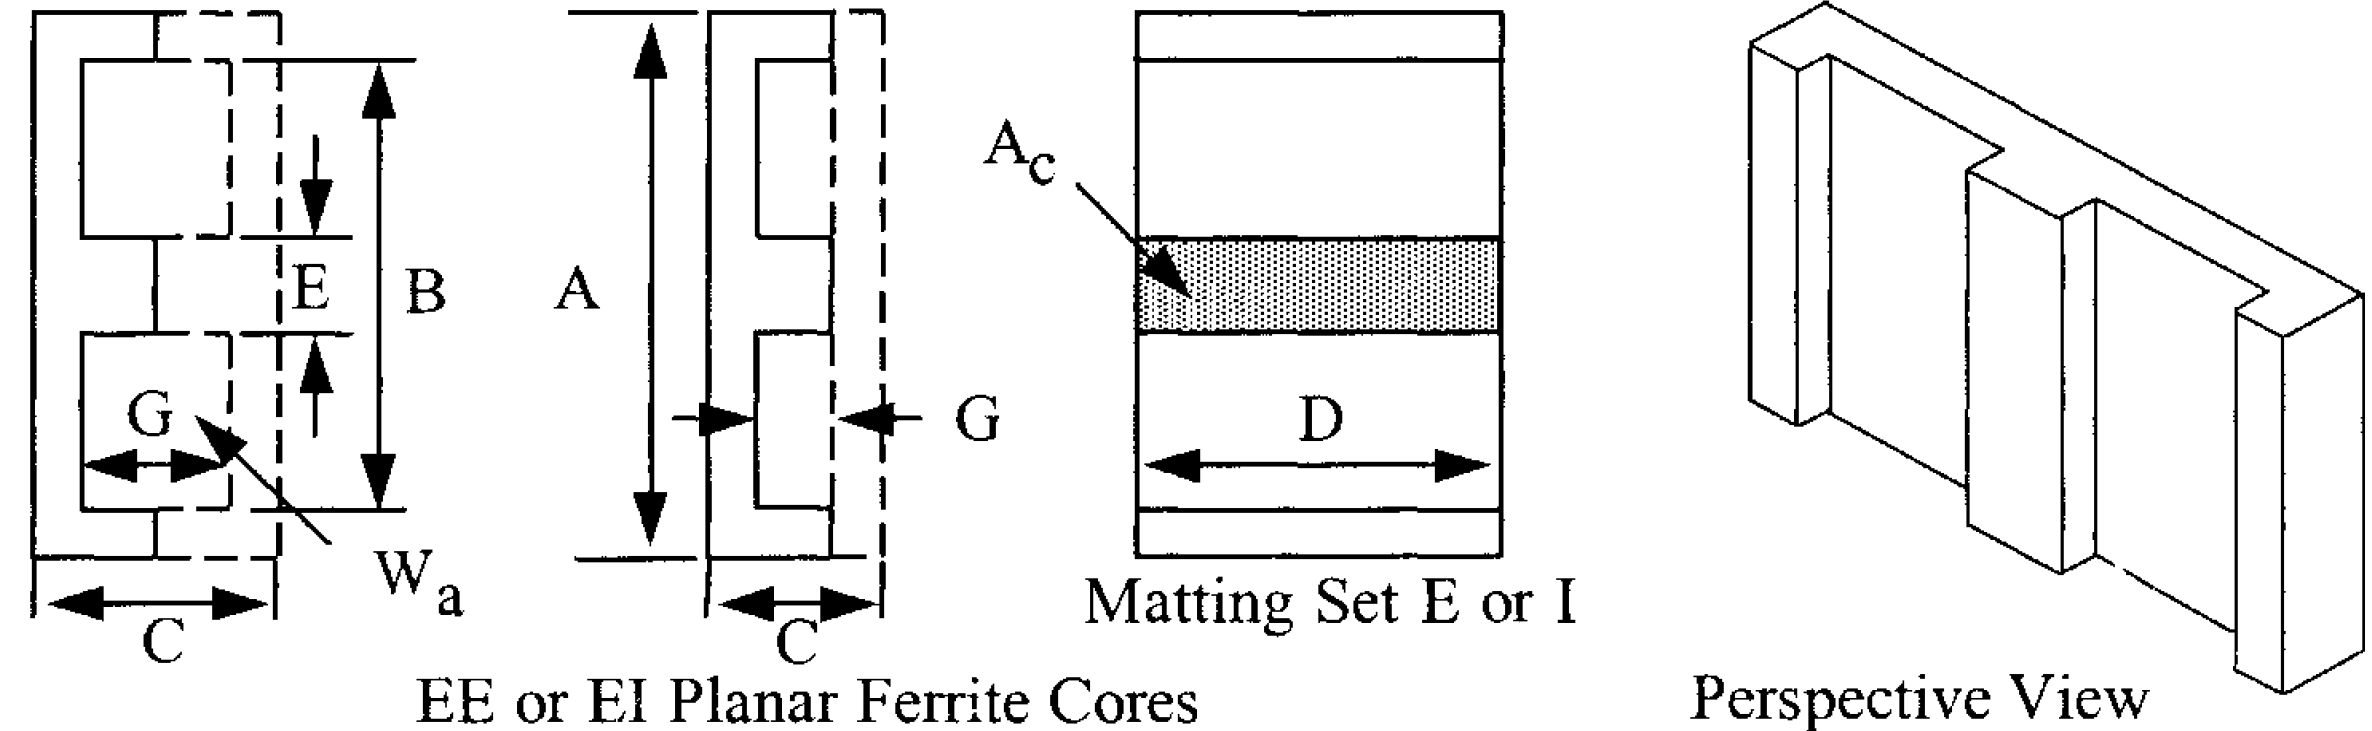
\includegraphics[width=0.75\linewidth]{fig/lec07/EE_core.png}
                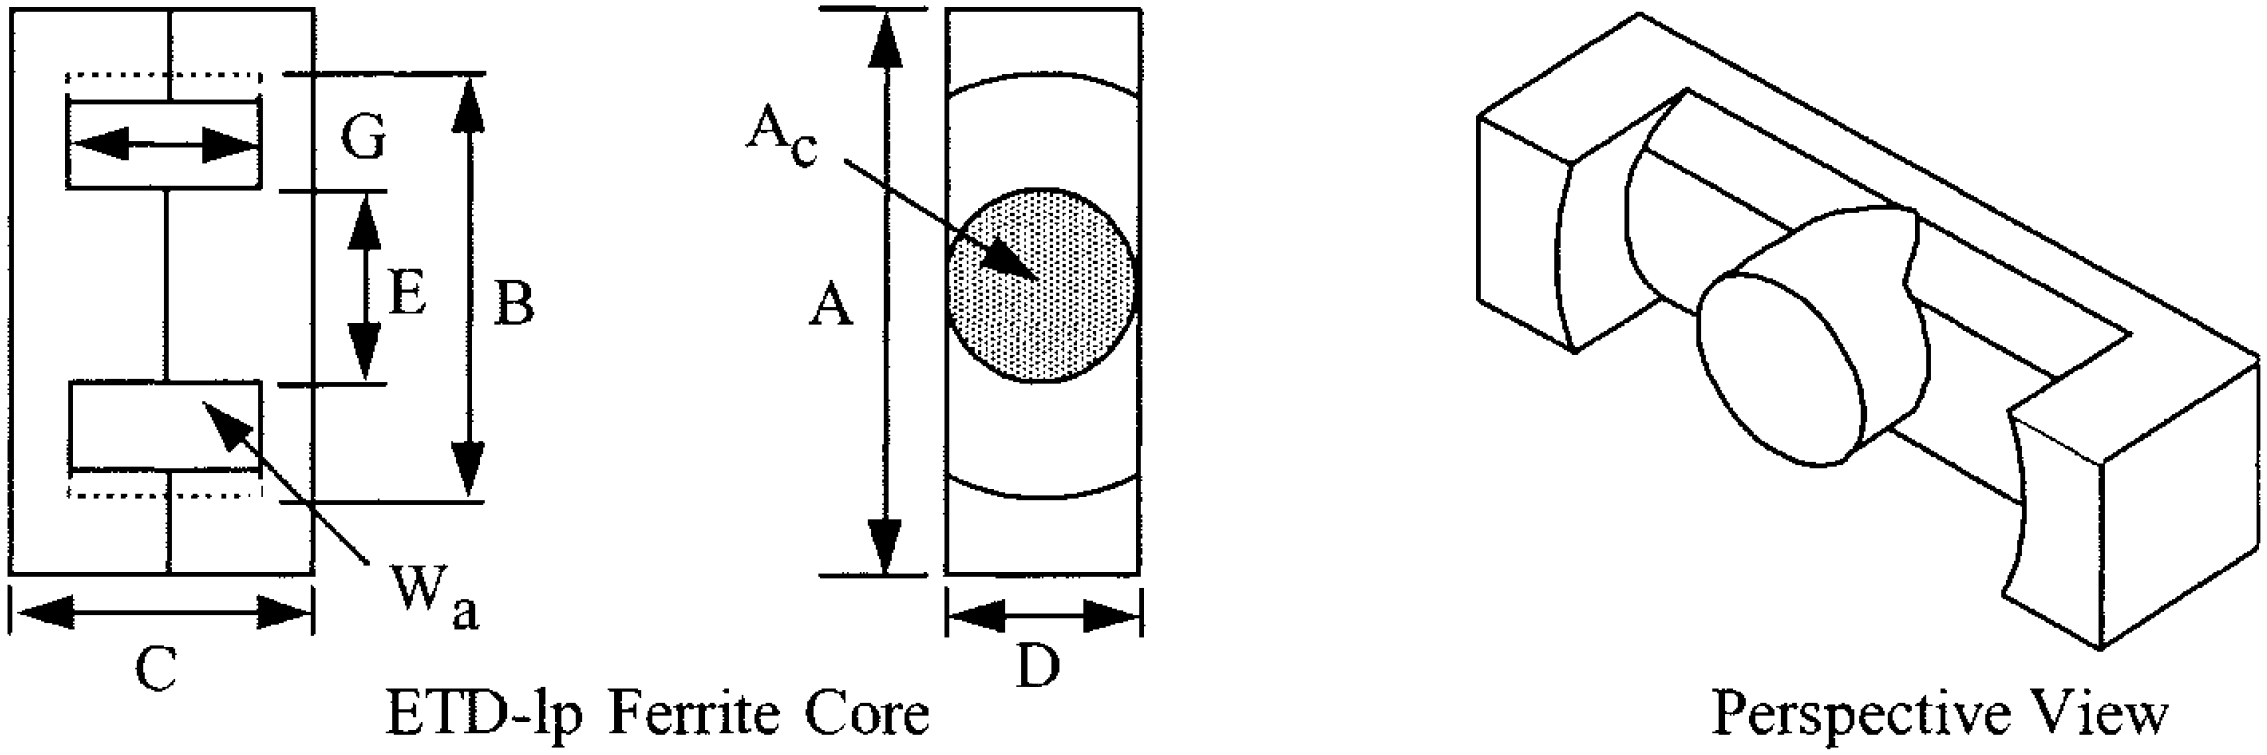
\includegraphics[width=0.75\linewidth]{fig/lec07/ETD_core.png}
              \caption{Low-profile planar core geometries including EE/EI, ER, ETD families. Adapted from \textit{Transformer and Inductor Design Handbook}}
            \end{figure}
        \end{column}

        \begin{column}{0.5\textwidth}
            \begin{figure}
                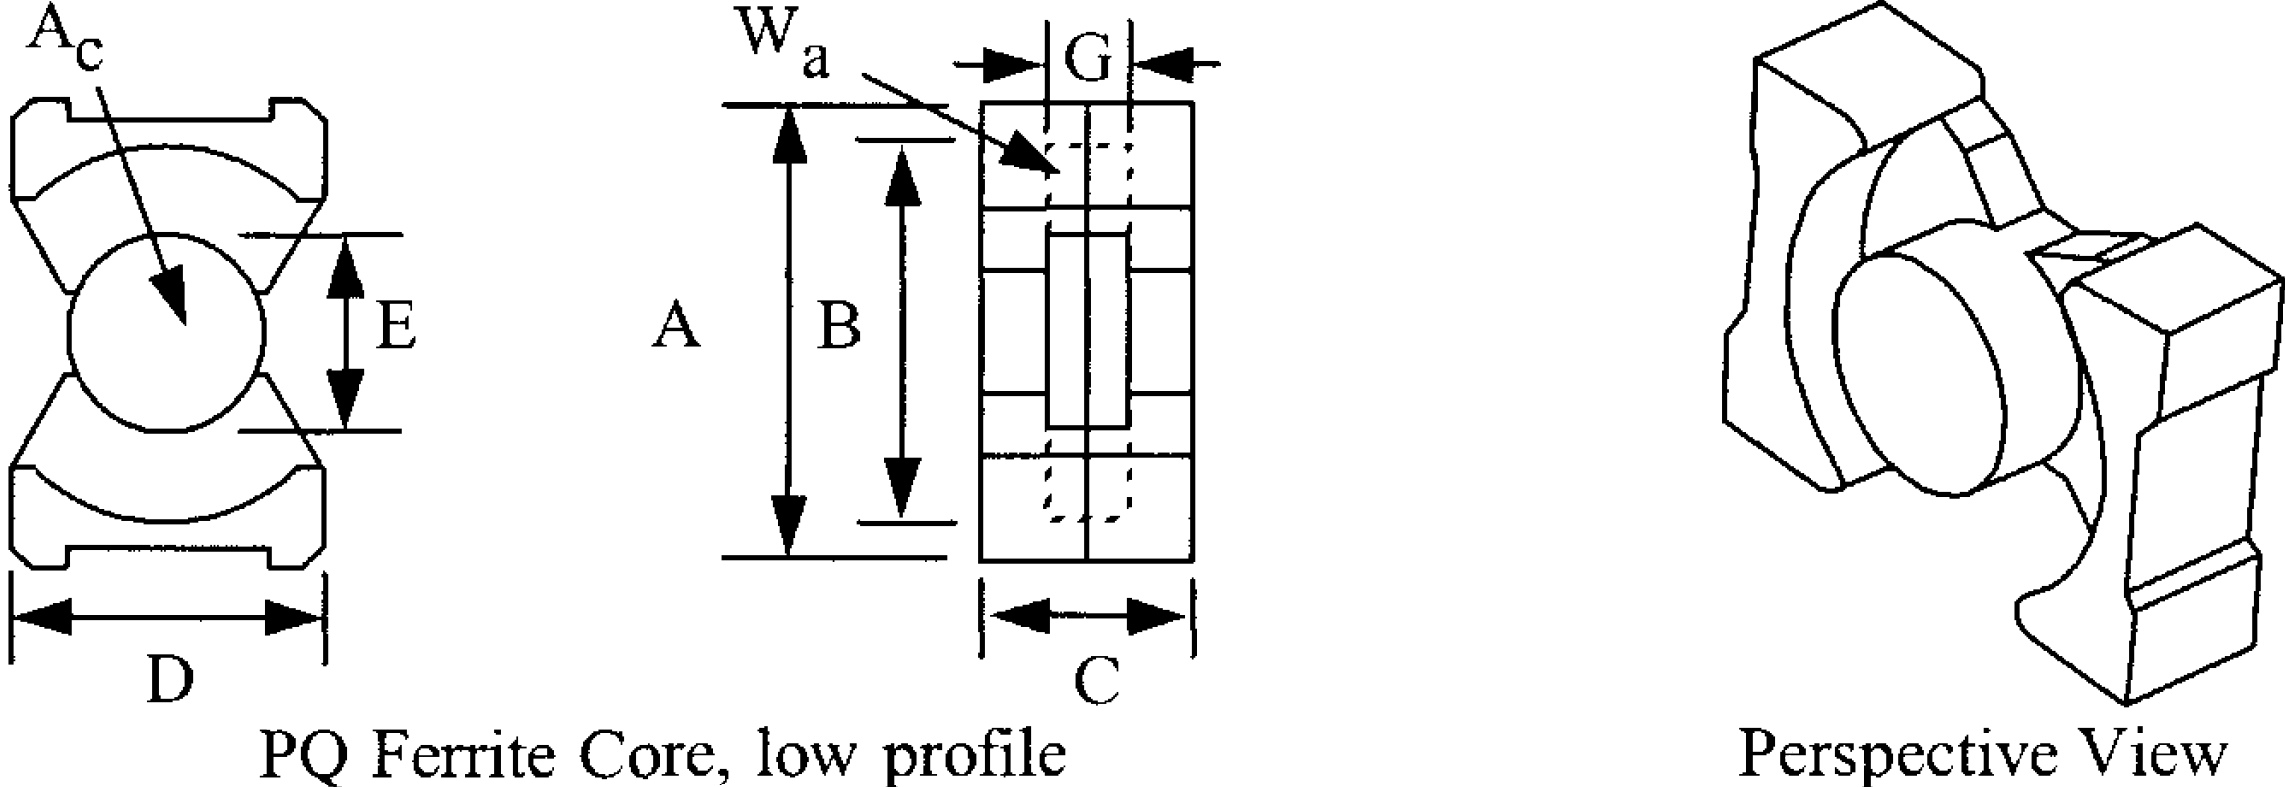
\includegraphics[width=0.75\linewidth]{fig/lec07/PQ_core.png}
                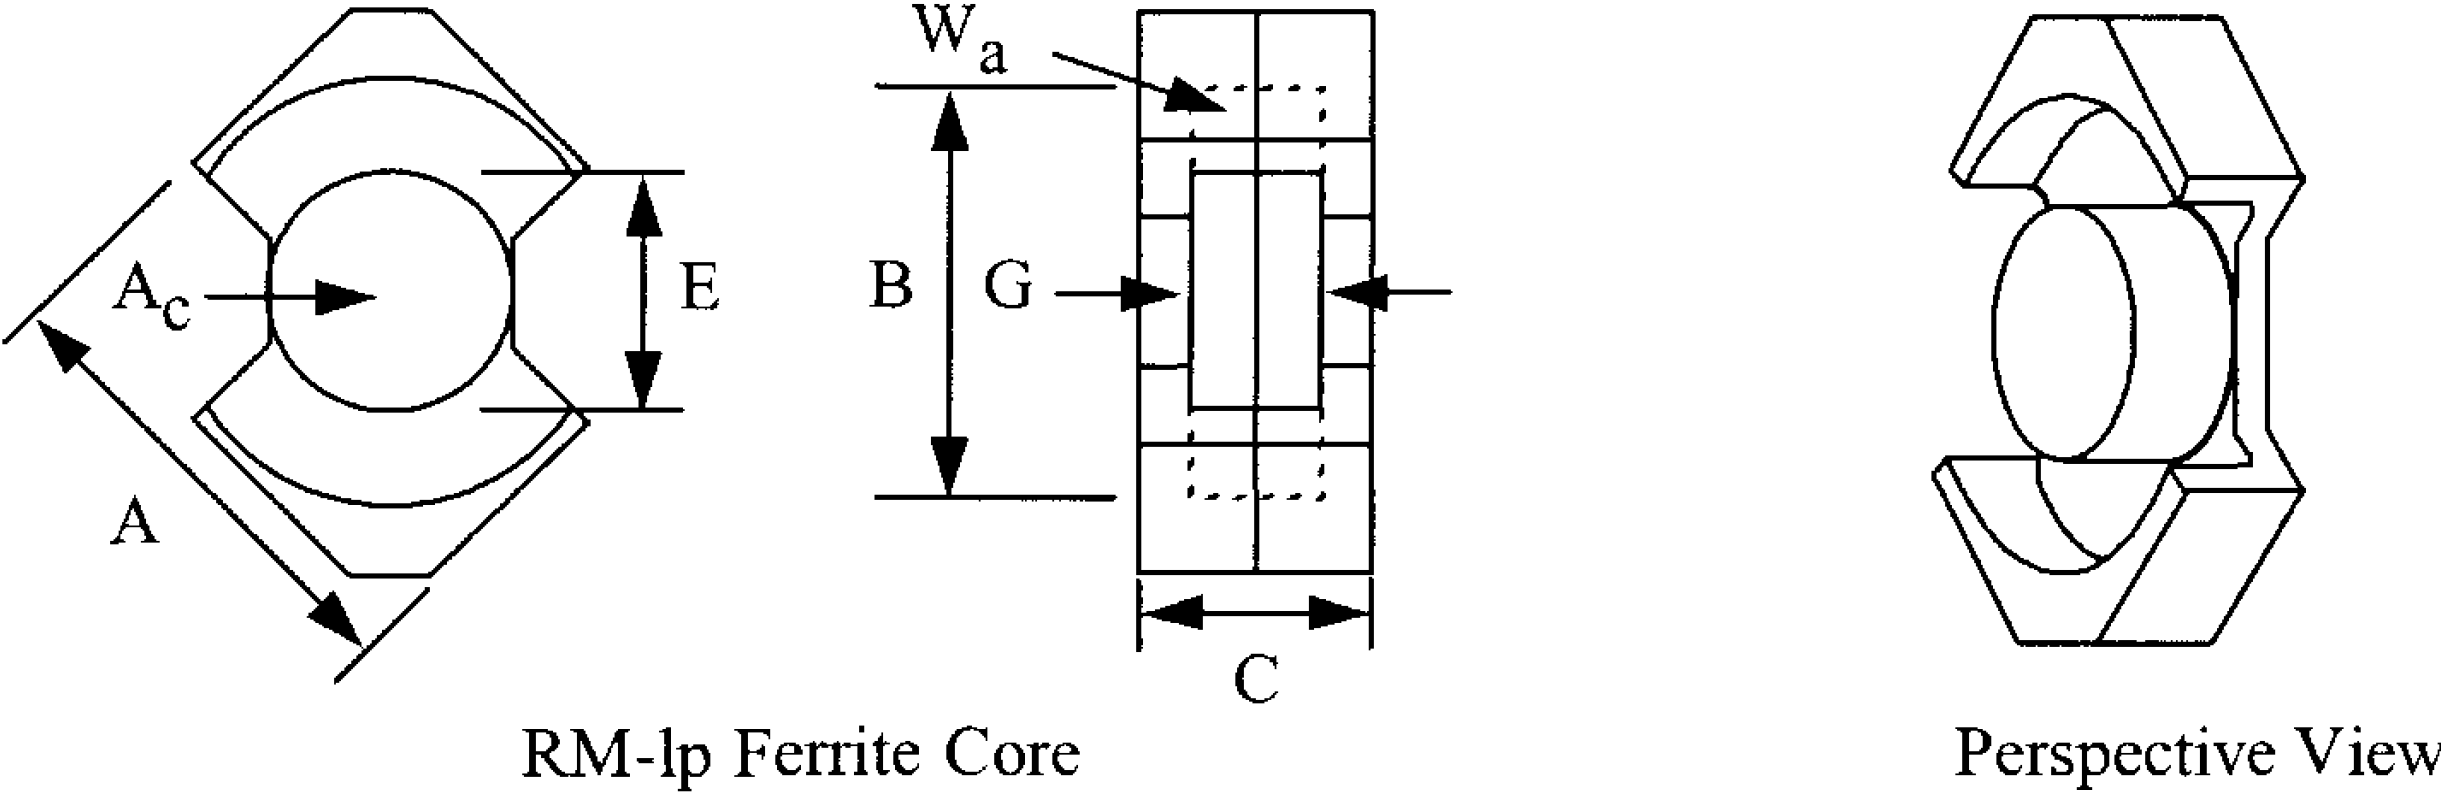
\includegraphics[width=0.5\linewidth]{fig/lec07/RM_core.png}
                \caption{Low-profile planar core geometries including PQ and RM families. Adapted from \textit{Transformer and Inductor Design Handbook}}
            \end{figure}
        \end{column}
    \end{columns}
\end{frame}
%%%%%%%%%%%%%%%%%%%%%%%%%%%%%%%%%%%%%%%%%%%%%%%%%%%%%%%%%%%%%
%% Area product and core size
%%%%%%%%%%%%%%%%%%%%%%%%%%%%%%%%%%%%%%%%%%%%%%%%%%%%%%%%%%%%%
\begin{frame}
    \frametitle{Area Product and Core-Size Selection}

    \begin{columns}
        \begin{column}{0.58\textwidth}
            The core must simultaneously satisfy magnetic and winding-space constraints. The area product is
            \begin{align}
                A_P = A_c A_w
            \end{align}

            where
            \begin{itemize}
                \item $A_c$ supports the required flux,
                \item $A_w$ provides space for the windings.
            \end{itemize}
            For transformer designs where core loss is important, a core geometrical constant $K_{gfe}$ is introduced as a first-pass sizing parameter:
            \begin{align}
                K_{gfe} \geq K_{gfe,\mathrm{req}}
            \end{align}
        \end{column}

        \begin{column}{0.38\textwidth}
            This approach using $K_{gfe}$ accounts for both copper loss and core loss in selecting a suitable core size.
            \begin{block}{Design Interpretation}
                \small
                At high frequency, transformer design is often not saturation-limited. It is frequently core-loss-limited, so the selected $\Delta B$ is much lower than $B_{\mathrm{sat}}$.
            \end{block}
        \end{column}
    \end{columns}
\end{frame}


%%%%%%%%%%%%%%%%%%%%%%%%%%%%%%%%%%%%%%%%%%%%%%%%%%%%%%%%%%%%%
%% Turns ratio and secondary turns
%%%%%%%%%%%%%%%%%%%%%%%%%%%%%%%%%%%%%%%%%%%%%%%%%%%%%%%%%%%%%
\begin{frame}
    \frametitle{Turns Ratio and Secondary Turns}

    \begin{columns}
        \begin{column}{0.58\textwidth}
            The turns ratio is selected from converter voltage gain and device-voltage stress requirements. For an ideal transformer,
            \begin{align}
                \frac{v_2}{v_1}=\frac{N_2}{N_1}=n
            \end{align}
            Once $N_1$ is selected from the volt-second constraint, the secondary turns are $N_2 = nN_1$.
            In practical design:
            \begin{itemize}
                \item $N_1$ and $N_2$ must be rounded to integers.
                \item Rounding changes the actual turns ratio.
                \item The new ratio must be checked against voltage gain and semiconductor stress.
                \item Multi-output transformers require additional secondary turns and regulation checks.
            \end{itemize}
        \end{column}

        \begin{column}{0.38\textwidth}
            \begin{figure}
                \centering
                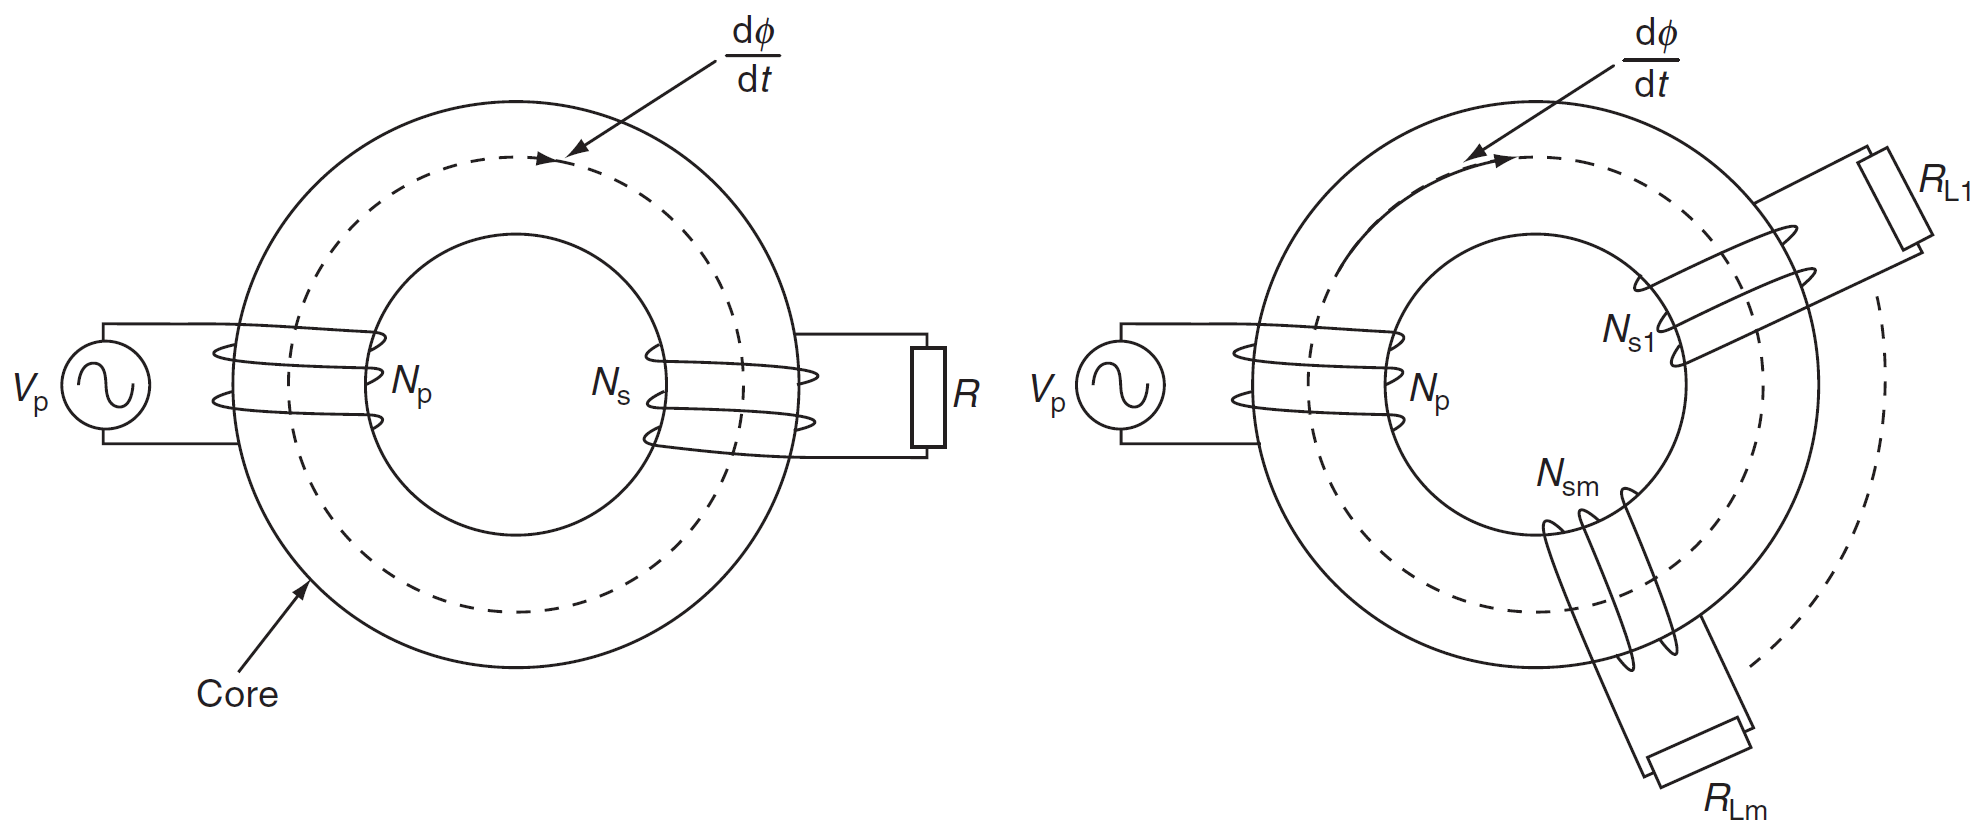
\includegraphics[width=\linewidth]{fig/lec07/trans_sec_winding.png}
                \caption{Single-secondary and multiple-secondary transformer structures. Adapted from Umanand, \textit{Power Electronics: Essentials and Applications}}
            \end{figure}
        \end{column}
    \end{columns}
\end{frame}


%%%%%%%%%%%%%%%%%%%%%%%%%%%%%%%%%%%%%%%%%%%%%%%%%%%%%%%%%%%%%
%% Winding area and current density
%%%%%%%%%%%%%%%%%%%%%%%%%%%%%%%%%%%%%%%%%%%%%%%%%%%%%%%%%%%%%
\begin{frame}
    \frametitle{Winding Area, Fill Factor, and Current Density}

    \begin{columns}
        \begin{column}{0.58\textwidth}
            After determining the turns, the winding must physically fit inside the available window area. The available copper area is $
                A_{\mathrm{Cu,available}} = K_u W_A$, 
            where $K_u$ is the window utilization or fill factor. For each winding,
            \begin{align}
                A_{w,j} \approx \frac{I_{j,\mathrm{rms}}}{J}
            \end{align}
            where $J$ is the allowable current density. The selected winding must satisfy:
            \begin{itemize}
                \item DC resistance limit
                \item AC resistance limit
                \item Temperature-rise limit
                \item Insulation and creepage/clearance limits
            \end{itemize}
        \end{column}

        \begin{column}{0.38\textwidth}
            \begin{figure}
                \centering
                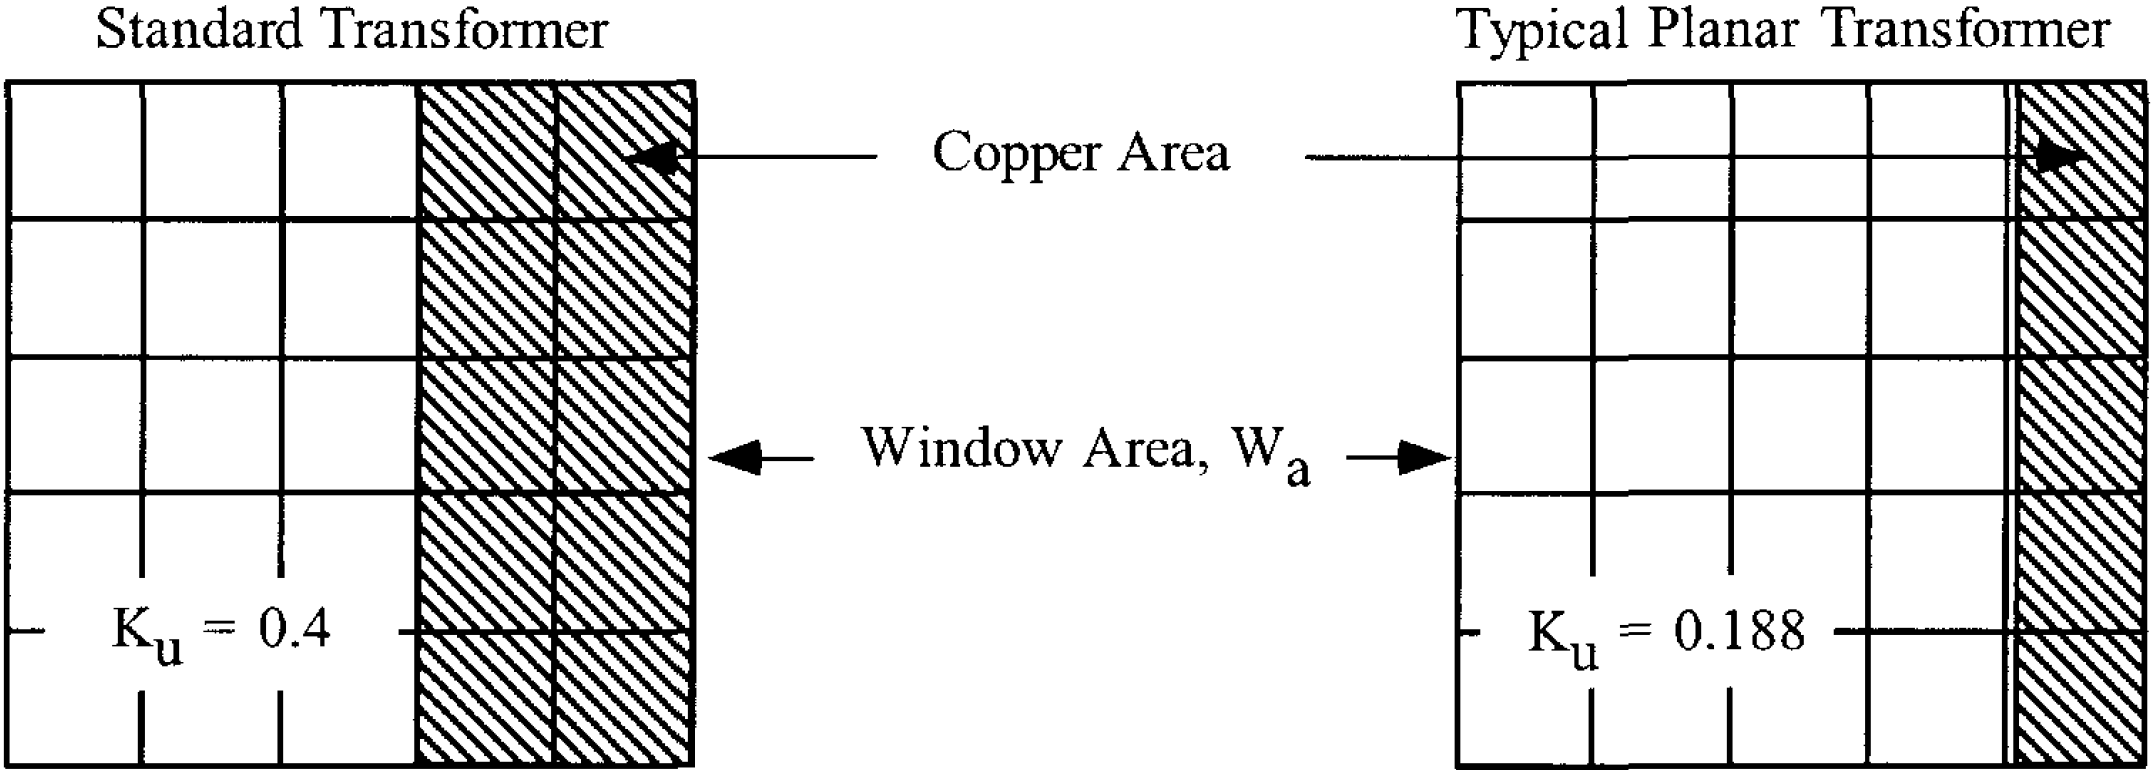
\includegraphics[width=\linewidth]{fig/lec07/window_uti.png}
                \caption{Comparison of window utilization in standard and planar transformers. Adapted from \textit{Transformer and Inductor Design Handbook}}
            \end{figure}
        \end{column}
    \end{columns}
\end{frame}


%%%%%%%%%%%%%%%%%%%%%%%%%%%%%%%%%%%%%%%%%%%%%%%%%%%%%%%%%%%%%
%% Planar transformer winding design
%%%%%%%%%%%%%%%%%%%%%%%%%%%%%%%%%%%%%%%%%%%%%%%%%%%%%%%%%%%%%
\begin{frame}
    \frametitle{Planar Transformer Winding Design}

    \begin{columns}
        \begin{column}{0.58\textwidth}
            In planar transformers, the winding is implemented using PCB copper, flexible PCB, stamped copper, or a hybrid structure.

            \vspace{0.15cm}

            The main winding decisions are:
            \begin{itemize}
                \item Copper thickness: 1 oz, 2 oz, 3 oz, or thicker copper
                \item Track width and spacing
                \item Number of PCB layers
                \item Via current capability
                \item Layer-to-layer insulation
                \item Primary-secondary arrangement
            \end{itemize}

            \vspace{0.15cm}

            Planar windings provide excellent repeatability and controlled parasitics, but they can suffer from low window utilization and high interwinding capacitance.
        \end{column}

        \begin{column}{0.38\textwidth}
            \begin{figure}
                \centering
                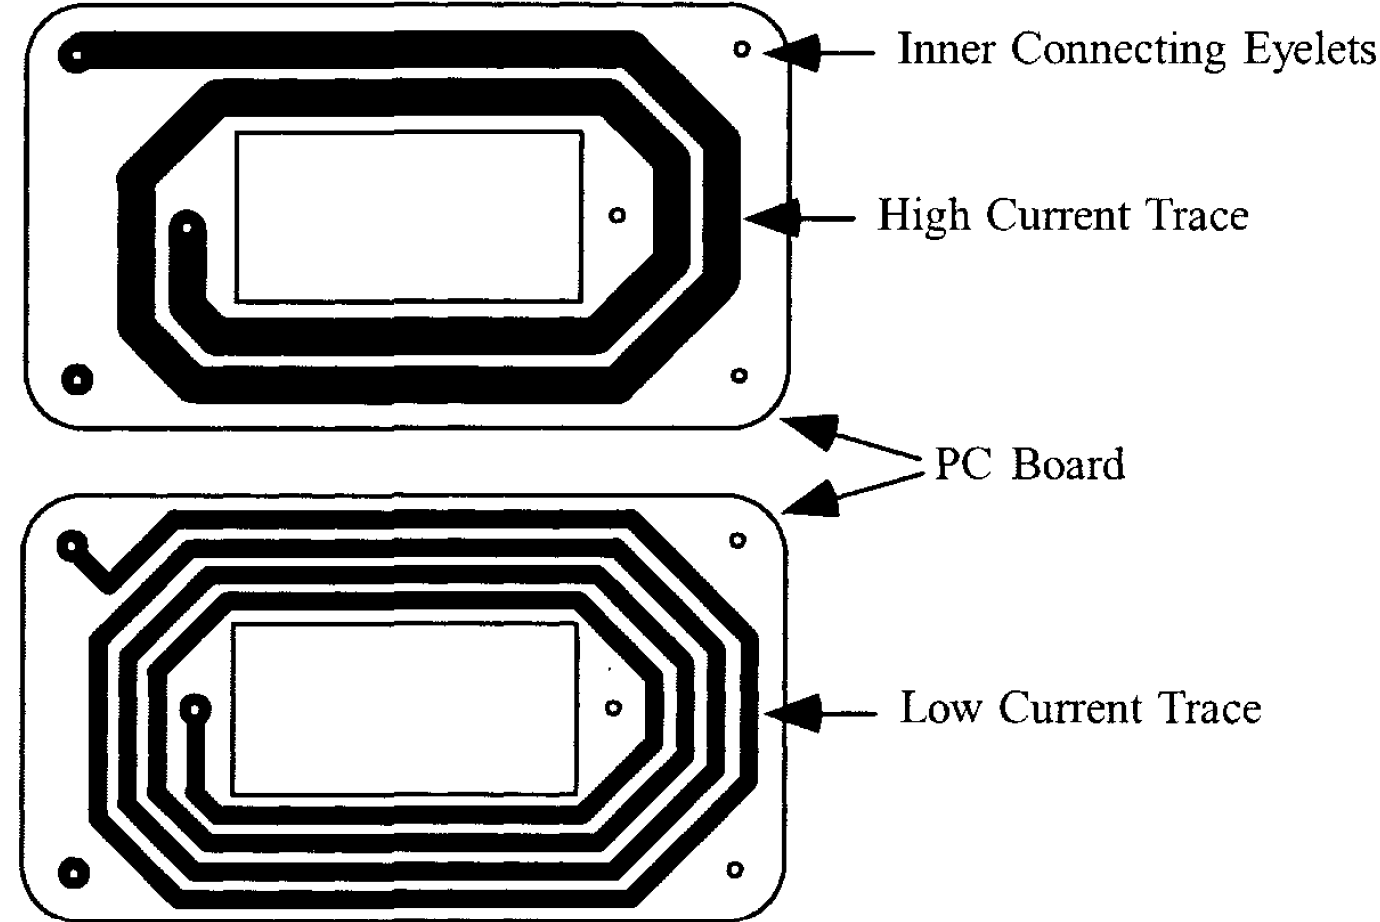
\includegraphics[width=\linewidth]{fig/lec07/planer_E_core_winding.png}
                \caption{Typical planar E-core winding PCB with high-current and low-current traces. Adapted from \textit{Transformer and Inductor Design Handbook}}
            \end{figure}
        \end{column}
    \end{columns}
\end{frame}


%%%%%%%%%%%%%%%%%%%%%%%%%%%%%%%%%%%%%%%%%%%%%%%%%%%%%%%%%%%%%
%% Leakage and magnetizing inductance check
%%%%%%%%%%%%%%%%%%%%%%%%%%%%%%%%%%%%%%%%%%%%%%%%%%%%%%%%%%%%%
\begin{frame}
    \frametitle{Magnetizing and Leakage Inductance Check}

    \begin{columns}
        \begin{column}{0.58\textwidth}
            After the first-pass design, the transformer must be checked using its equivalent circuit. The magnetizing inductance is approximately $L_M = \frac{N_1^2}{\mathcal{R}}$, and determines the magnetizing current:
            \begin{align}
                i_M(t)=\frac{1}{L_M}\int v_1(t)\,dt
            \end{align}
            Leakage inductance appears in series with the windings and affects:
            \begin{itemize}
                \item Voltage spikes
                \item Current transfer
                \item Ringing frequency
                \item Resonant-tank behaviour
                \item Snubber or clamp design
            \end{itemize}
        \end{column}

        \begin{column}{0.38\textwidth}
            \begin{figure}
                \centering
                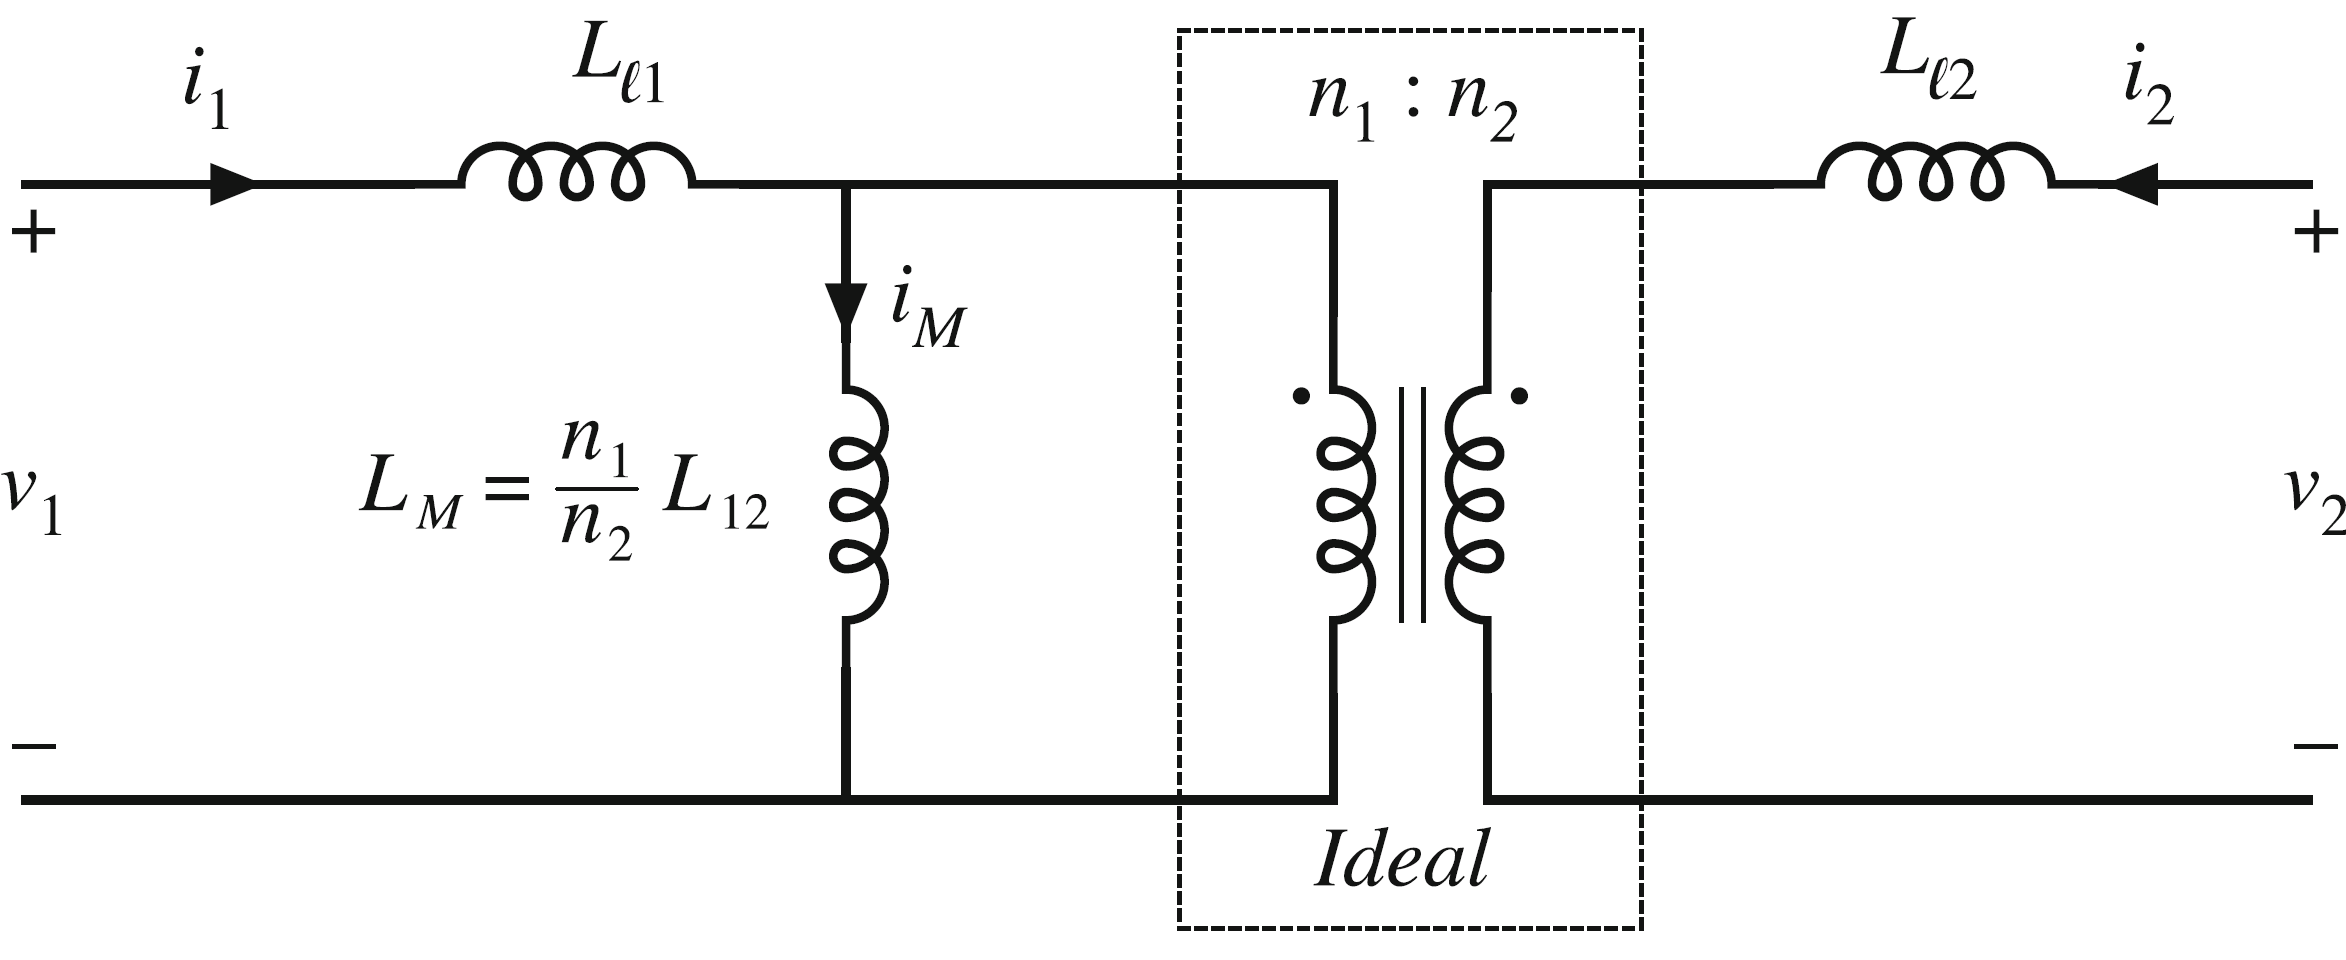
\includegraphics[width=\linewidth]{fig/lec07/transformer_equivalent_circuit.png}
                \caption{Two-winding transformer equivalent circuit including magnetizing inductance and primary/secondary leakage inductances. Adapted from Erickson and Maksimovi\'c, \textit{Fundamentals of Power Electronics}, 3rd edition}
            \end{figure}
        \end{column}
    \end{columns}
\end{frame}


%%%%%%%%%%%%%%%%%%%%%%%%%%%%%%%%%%%%%%%%%%%%%%%%%%%%%%%%%%%%%
%% Design verification and iteration
%%%%%%%%%%%%%%%%%%%%%%%%%%%%%%%%%%%%%%%%%%%%%%%%%%%%%%%%%%%%%
\begin{frame}
    \frametitle{Transformer Design Verification}

    \begin{columns}
        \begin{column}{0.58\textwidth}
            A transformer design is acceptable only after electrical, magnetic, thermal, and insulation checks are satisfied.

            \vspace{0.15cm}

            Minimum verification checklist:
            \begin{itemize}
                \item Flux density:
                \[
                    \Delta B < \Delta B_{\max}
                \]
                \item Core loss from material loss curves or Steinmetz model
                \item DC and AC copper losses
                \item Leakage inductance and parasitic capacitance
                \item Temperature rise at worst-case operation
                \item Isolation, creepage and clearance
                \item Manufacturability and repeatability
            \end{itemize}

        \end{column}

        \begin{column}{0.38\textwidth}
        High-frequency transformers usually require several design iterations.
            \begin{block}{First-Pass Design is Not Final}
                \small
                Analytical equations select a candidate core and turns. Final design requires loss estimation, thermal validation, parasitic extraction, and experimental measurement.
            \end{block}
        \end{column}
    \end{columns}
\end{frame}

%%%%%%%%%%%%%%%%%%%%%%%%%%%%%%%%%%%%%%%%%%%%%%%%%%%%%%%%%%%%%
%% Module 3
%%%%%%%%%%%%%%%%%%%%%%%%%%%%%%%%%%%%%%%%%%%%%%%%%%%%%%%%%%%%%
\begin{frame}
\begin{center}
  \textbf{\Huge{Winding Arrangements}}\\[0.4cm]
  \textbf{\Large{Leakage, AC Resistance, Capacitance, and Manufacturability}}
\end{center}
\end{frame}


%%%%%%%%%%%%%%%%%%%%%%%%%%%%%%%%%%%%%%%%%%%%%%%%%%%%%%%%%%%%%
%% Why winding arrangement matters
%%%%%%%%%%%%%%%%%%%%%%%%%%%%%%%%%%%%%%%%%%%%%%%%%%%%%%%%%%%%%
\begin{frame}
    \frametitle{Why Winding Arrangement Matters}

    \begin{columns}
        \begin{column}{0.58\textwidth}
            In high-frequency magnetic components, the winding arrangement is often as important as the core material. It directly influences:
            \begin{itemize}
                \item Leakage inductance
                \item Proximity-effect loss
                \item Skin-effect loss
                \item Interwinding capacitance
                \item Common-mode noise
                \item Thermal path from copper to ambient
                \item Manufacturability and repeatability
            \end{itemize}
            In low-frequency transformers, winding design is mainly about copper area and insulation. In high-frequency power electronics, it is also about controlling the magnetic field distribution inside the winding window.
        \end{column}

        \begin{column}{0.38\textwidth}
            \begin{block}{Design Message}
                \small
                A transformer with the correct turns ratio can still perform poorly if the winding layout produces excessive leakage inductance, AC resistance, or parasitic capacitance.
            \end{block}
        \end{column}
    \end{columns}
\end{frame}


%%%%%%%%%%%%%%%%%%%%%%%%%%%%%%%%%%%%%%%%%%%%%%%%%%%%%%%%%%%%%
%% Layered winding
%%%%%%%%%%%%%%%%%%%%%%%%%%%%%%%%%%%%%%%%%%%%%%%%%%%%%%%%%%%%%
\begin{frame}
    \frametitle{Layered Winding}

    \begin{columns}
        \begin{column}{0.58\textwidth}
            A layered winding places one winding layer after another inside the core window. This is simple and manufacturable, but it may produce high leakage inductance and high proximity loss. Typical structure:
            \begin{itemize}
                \item Primary layers grouped together
                \item Secondary layers grouped together
                \item Insulation placed between primary and secondary
            \end{itemize}

        \end{column}

        \begin{column}{0.38\textwidth}
            \begin{figure}
                \centering
                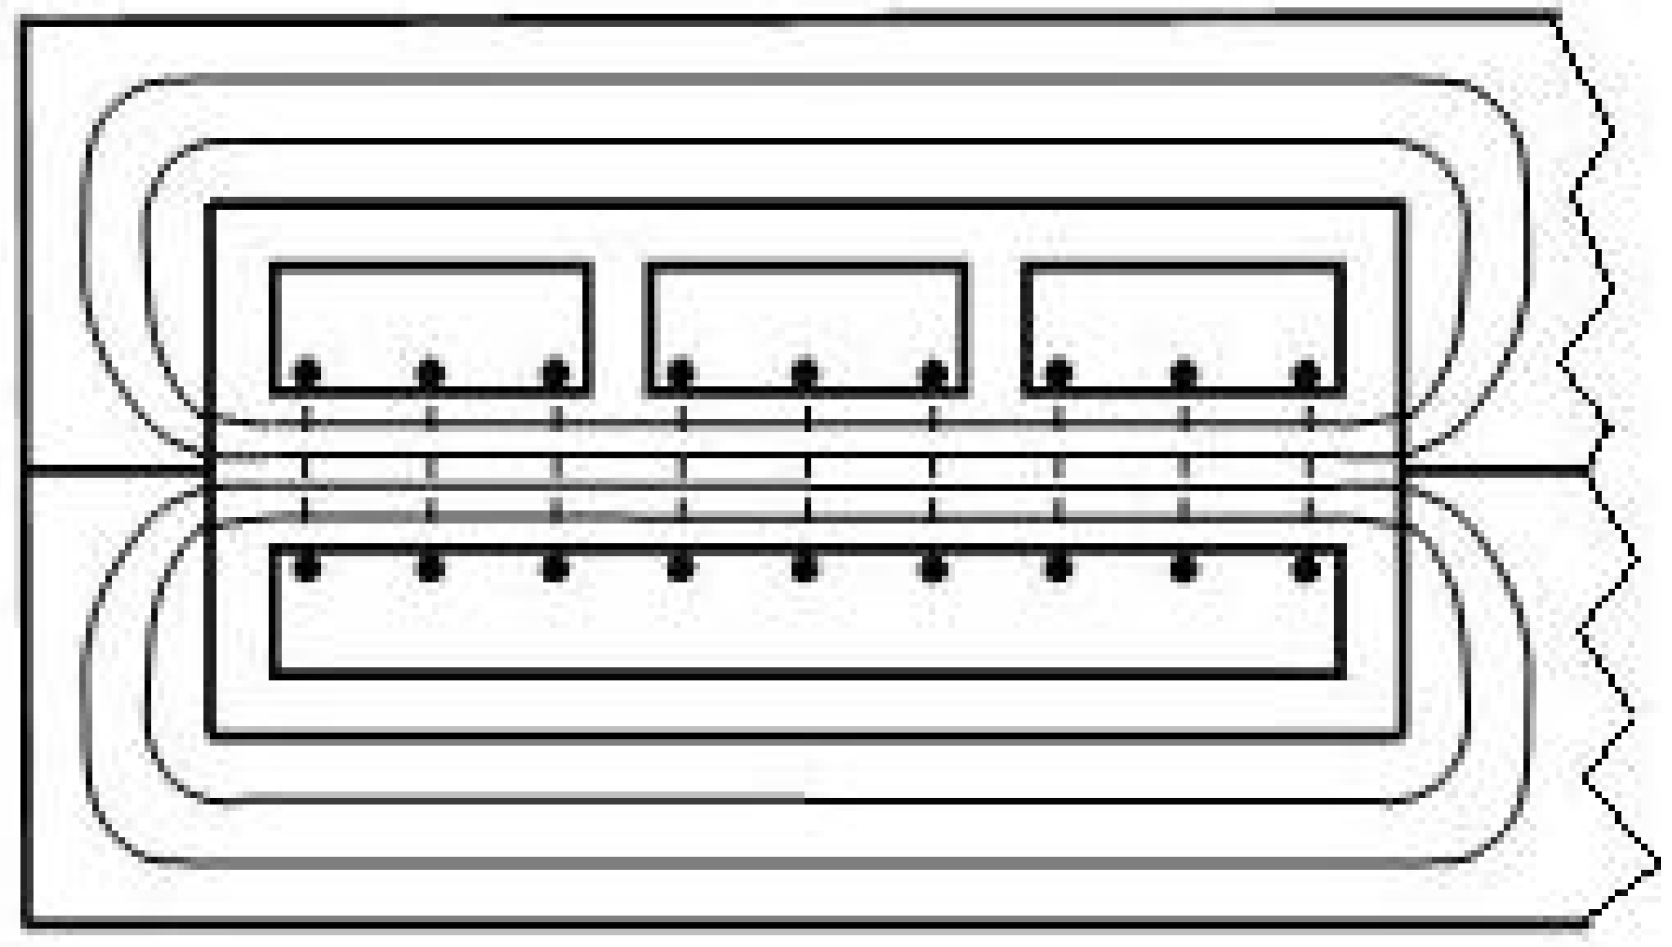
\includegraphics[width=\linewidth]{fig/lec07/planar_transformer_flux.png}
                \caption{Magnetic force equipotentials and leakage flux lines between primary and secondary windings in a planar transformer. Adapted from Dixon, Texas Instruments, \textit{Designing Planar Magnetics}}
            \end{figure}
        \end{column}
    \end{columns}
\end{frame}

%%%%%%%%%%%%%%%%%%%%%%%%%%%%%%%%%%%%%%%%%%%%%%%%%%%%%%%%%%%%%
%% Layered winding
%%%%%%%%%%%%%%%%%%%%%%%%%%%%%%%%%%%%%%%%%%%%%%%%%%%%%%%%%%%%%
\begin{frame}
    \frametitle{Layered Winding}

    \begin{columns}
        \begin{column}{0.58\textwidth}
            Advantages:
            \begin{itemize}
                \item Simple construction
                \item Good insulation control
                \item Easy to manufacture
            \end{itemize}

            Limitations:
            \begin{itemize}
                \item Larger leakage field between winding groups
                \item Increased AC winding resistance
                \item Poorer transient behaviour in hard-switched converters
            \end{itemize}
        \end{column}

        \begin{column}{0.38\textwidth}
            \begin{figure}
                \centering
                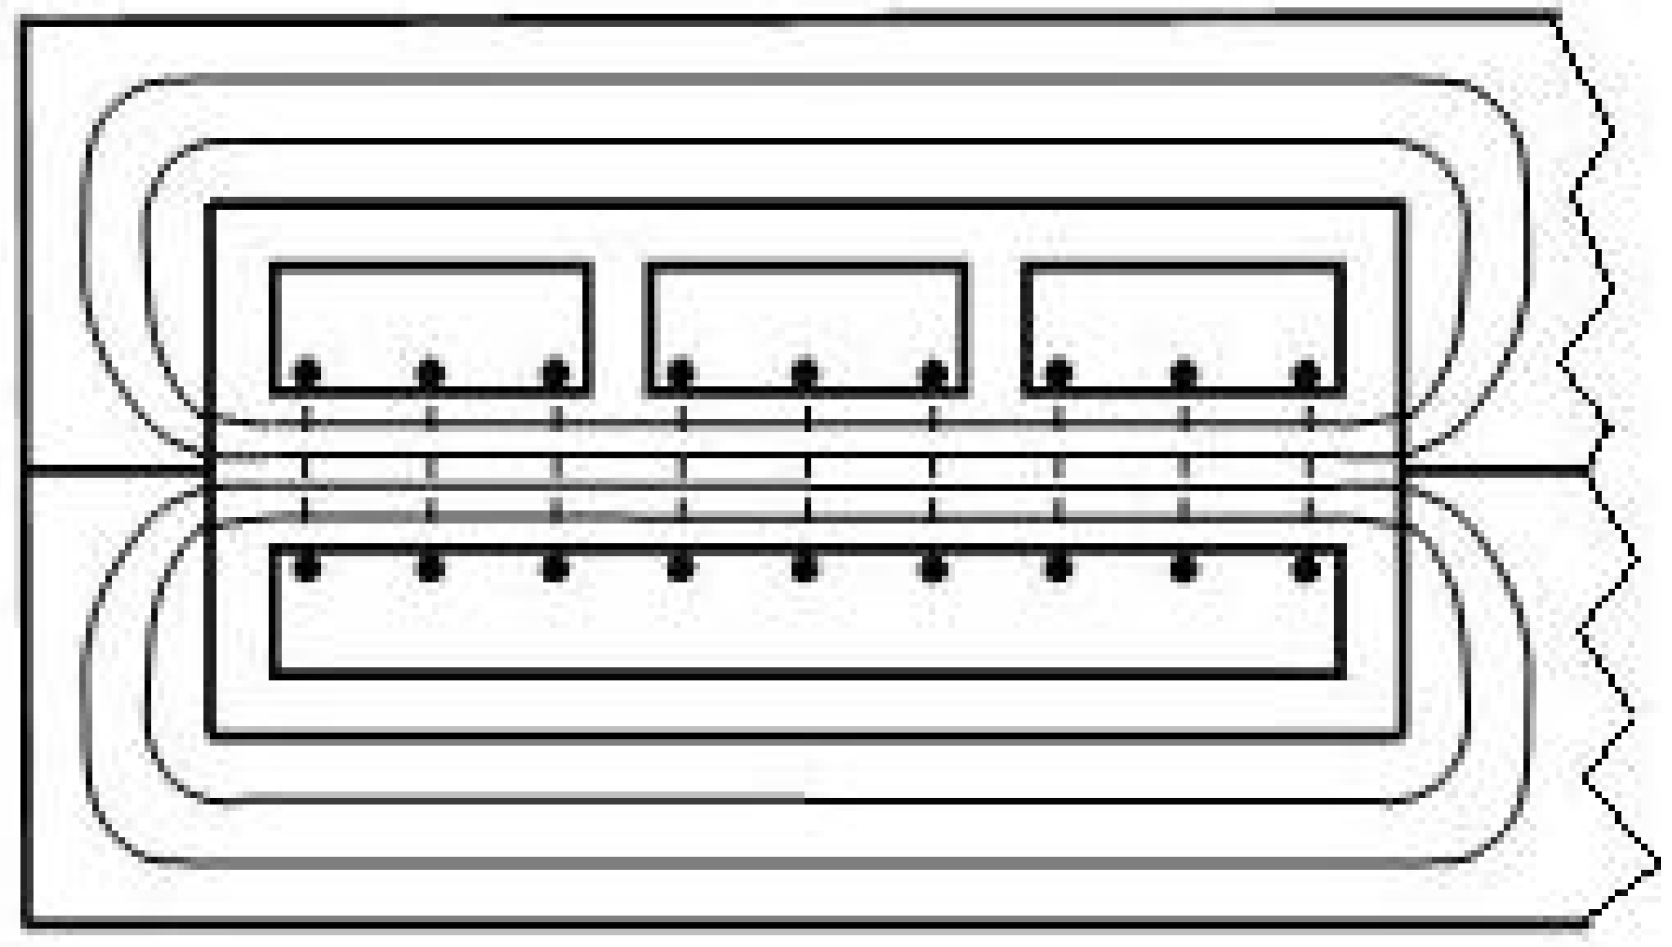
\includegraphics[width=\linewidth]{fig/lec07/planar_transformer_flux.png}
                \caption{Magnetic force equipotentials and leakage flux lines between primary and secondary windings in a planar transformer. Adapted from Dixon, Texas Instruments, \textit{Designing Planar Magnetics}}
            \end{figure}
        \end{column}
    \end{columns}
\end{frame}

%%%%%%%%%%%%%%%%%%%%%%%%%%%%%%%%%%%%%%%%%%%%%%%%%%%%%%%%%%%%%
%% Sectional winding
%%%%%%%%%%%%%%%%%%%%%%%%%%%%%%%%%%%%%%%%%%%%%%%%%%%%%%%%%%%%%
\begin{frame}
    \frametitle{Sectional Winding}

    \begin{columns}
        \begin{column}{0.58\textwidth}
            In sectional winding, the winding is divided into sections rather than being placed as one continuous block. The purpose is to control the spatial distribution of magnetic field and electric field inside the winding window.
            Sectional winding can be useful when:
            \begin{itemize}
                \item High isolation voltage is required
                \item Interwinding capacitance must be reduced
                \item Leakage inductance must be intentionally adjusted
                \item Multiple outputs require physical separation
            \end{itemize}

            Compared with full interleaving, sectional winding may increase leakage inductance, but can reduce capacitance and simplify insulation design.
        \end{column}

        \begin{column}{0.38\textwidth}
            \begin{block}{Engineering Trade-off}
                \small
                Interleaving generally reduces leakage inductance but increases capacitance.

                \vspace{0.15cm}

                Sectionalization generally reduces capacitance and improves insulation control but can increase leakage inductance.
            \end{block}
        \end{column}
    \end{columns}
\end{frame}


%%%%%%%%%%%%%%%%%%%%%%%%%%%%%%%%%%%%%%%%%%%%%%%%%%%%%%%%%%%%%
%% Interleaved winding
%%%%%%%%%%%%%%%%%%%%%%%%%%%%%%%%%%%%%%%%%%%%%%%%%%%%%%%%%%%%%
\begin{frame}
    \frametitle{Interleaved Winding}

    \begin{columns}
        \begin{column}{0.55\textwidth}
            Interleaving alternates primary and secondary winding sections to reduce the magnetic field energy stored between them. Examples:
            \begin{itemize}
                \item P--S--P
                \item S--P--S
                \item P--S--P--S
                \item PCB layer interleaving in planar transformers
            \end{itemize}
            Main benefits:
            \begin{itemize}
                \item Reduced leakage inductance
                \item Reduced voltage overshoot
                \item Better current transfer
                \item Lower proximity-effect loss in many transformer cases
            \end{itemize}
        \end{column}

        \begin{column}{0.44\textwidth}
            \begin{figure}
                \centering
                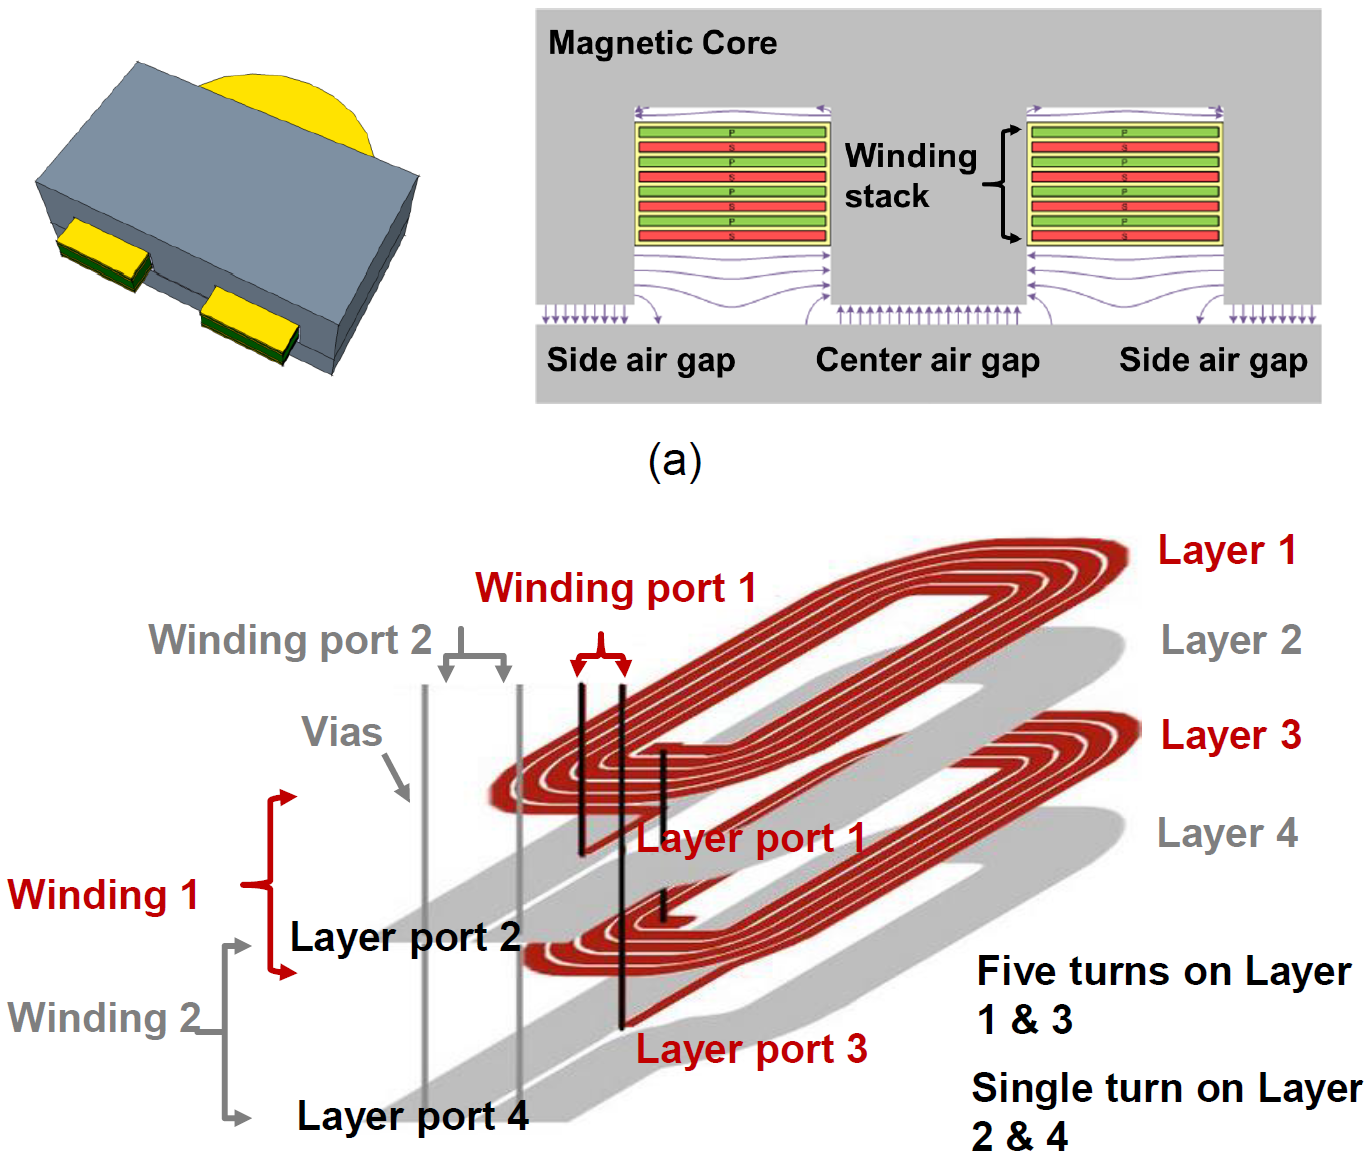
\includegraphics[width=0.8\linewidth]{fig/lec07/planar_winding_stack.png}
                \caption{Planar winding stack with multiple layers, winding ports and vias, illustrating how PCB layers can be connected and interleaved. Adapted from Chen et al., \textit{A Systematic Approach to Modeling Impedances and Current Distribution in Planar Magnetics}}
            \end{figure}
        \end{column}
    \end{columns}
However, interleaving can increase interwinding capacitance and common-mode noise.
\end{frame}


%%%%%%%%%%%%%%%%%%%%%%%%%%%%%%%%%%%%%%%%%%%%%%%%%%%%%%%%%%%%%
%% Foil winding
%%%%%%%%%%%%%%%%%%%%%%%%%%%%%%%%%%%%%%%%%%%%%%%%%%%%%%%%%%%%%
\begin{frame}
    \frametitle{Foil Winding}

    \begin{columns}
        \begin{column}{0.58\textwidth}
            Foil windings use wide, thin copper conductors instead of round wires.

            \vspace{0.15cm}

            They are attractive for high-current windings because:
            \begin{itemize}
                \item DC resistance can be low
                \item Current can be spread over a wide conductor surface
                \item Thermal contact area is large
                \item Winding height can be compact
            \end{itemize}

            \vspace{0.15cm}

            The conductor thickness must be selected carefully. If the foil is much thicker than the skin depth, the inner copper is poorly used at high frequency.

            \begin{align}
                \delta = \sqrt{\frac{2\rho}{\omega \mu}}
            \end{align}
        \end{column}

        \begin{column}{0.38\textwidth}
            Foil windings are therefore useful when the foil thickness is comparable to, or smaller than, the relevant skin depth.
            \begin{block}{Design Rule}
                \small
                Foil width reduces DC resistance, but foil thickness controls high-frequency AC resistance.

                \vspace{0.15cm}

                Thin, wide copper is usually preferable to thick copper for high-frequency transformer windings.
            \end{block}
        \end{column}
    \end{columns}
\end{frame}


%%%%%%%%%%%%%%%%%%%%%%%%%%%%%%%%%%%%%%%%%%%%%%%%%%%%%%%%%%%%%
%% Litz, foil, PCB comparison
%%%%%%%%%%%%%%%%%%%%%%%%%%%%%%%%%%%%%%%%%%%%%%%%%%%%%%%%%%%%%
\begin{frame}
    \frametitle{Comparison of Round Wire, Foil, Litz, and PCB Windings}

    \scriptsize
    \begin{table}
        \centering
        \begin{tabular}{p{0.18\textwidth}p{0.20\textwidth}p{0.25\textwidth}p{0.25\textwidth}}
            \hline
            \textbf{Winding} & \textbf{Main Strength} & \textbf{Main Limitation} & \textbf{Typical Use}\\
            \hline
            Round wire & Simple and low cost & High AC loss at high frequency & Low-frequency and low-power magnetics\\
            Foil & Low DC resistance and good thermal area & Proximity loss if poorly arranged & High-current transformer windings\\
            Litz wire & Reduced skin and proximity effects & Cost, termination complexity & Resonant and MHz-range magnetics\\
            PCB winding & Repeatable and low profile & Low fill factor and high capacitance & Planar transformers and integrated magnetics\\
            \hline
        \end{tabular}
    \end{table}

    \vspace{0.15cm}

    \begin{block}{Message}
        \small
        The best winding technology depends on frequency, current, voltage isolation, manufacturing volume, leakage requirement, and thermal path.
    \end{block}
\end{frame}


%%%%%%%%%%%%%%%%%%%%%%%%%%%%%%%%%%%%%%%%%%%%%%%%%%%%%%%%%%%%%
%% Module 4
%%%%%%%%%%%%%%%%%%%%%%%%%%%%%%%%%%%%%%%%%%%%%%%%%%%%%%%%%%%%%
\begin{frame}
\begin{center}
  \textbf{\Huge{Magnetic Losses}}\\[0.4cm]
  \textbf{\Large{Core Loss, Copper Loss, and High-Frequency Effects}}
\end{center}
\end{frame}


%%%%%%%%%%%%%%%%%%%%%%%%%%%%%%%%%%%%%%%%%%%%%%%%%%%%%%%%%%%%%
%% Loss map
%%%%%%%%%%%%%%%%%%%%%%%%%%%%%%%%%%%%%%%%%%%%%%%%%%%%%%%%%%%%%
\begin{frame}
    \frametitle{Loss Mechanisms in Magnetic Components}

    \begin{center}
    \begin{circuitikz}[scale=0.78, transform shape]
        \tikzstyle{block} = [draw, rounded corners, align=center,
        minimum width=3.0cm, minimum height=0.8cm]

        \node[block] (total) at (4,0) {Total magnetic\\component loss};
        \node[block] (core) at (0,-1.7) {Core loss};
        \node[block] (copper) at (4,-1.7) {Copper loss};
        \node[block] (parasitic) at (8,-1.7) {Parasitic-related\\loss};

        \node[block] (hyst) at (-1.5,-3.4) {Hysteresis};
        \node[block] (eddy) at (1.5,-3.4) {Core eddy\\current};

        \node[block] (dc) at (3,-3.4) {DC winding\\loss};
        \node[block] (ac) at (5.2,-3.4) {AC winding\\loss};

        \node[block] (skin) at (3.8,-5.1) {Skin effect};
        \node[block] (prox) at (6.2,-5.1) {Proximity effect};

        \draw[->, thick] (total) -- (core);
        \draw[->, thick] (total) -- (copper);
        \draw[->, thick] (total) -- (parasitic);
        \draw[->, thick] (core) -- (hyst);
        \draw[->, thick] (core) -- (eddy);
        \draw[->, thick] (copper) -- (dc);
        \draw[->, thick] (copper) -- (ac);
        \draw[->, thick] (ac) -- (skin);
        \draw[->, thick] (ac) -- (prox);
    \end{circuitikz}
    \end{center}

    \vspace{0.1cm}

    \begin{block}{Teaching Message}
        \small
        At low frequency, DC copper loss and saturation may dominate. At high frequency, core loss, skin effect, proximity effect, leakage energy, and capacitance-related effects become increasingly important.
    \end{block}
\end{frame}


%%%%%%%%%%%%%%%%%%%%%%%%%%%%%%%%%%%%%%%%%%%%%%%%%%%%%%%%%%%%%
%% Core loss
%%%%%%%%%%%%%%%%%%%%%%%%%%%%%%%%%%%%%%%%%%%%%%%%%%%%%%%%%%%%%
\begin{frame}
    \frametitle{Core Loss}

    \begin{columns}
        \begin{column}{0.58\textwidth}
            Core loss is the heat generated inside the magnetic material during cyclic magnetization. The main components are:
            \begin{itemize}
                \item Hysteresis loss
                \item Eddy-current loss
                \item Excess or residual loss
            \end{itemize}
            Hysteresis loss is related to the energy required to reverse magnetic domains. Eddy-current loss is caused by induced circulating currents in conductive core material. A common empirical representation is the Steinmetz form:
            \begin{align}
                P_v = k f^{\alpha} B_{\mathrm{pk}}^{\beta}
            \end{align}
            where $P_v$ is the volumetric core-loss density.
        \end{column}

        \begin{column}{0.38\textwidth}
            \begin{block}{Practical Meaning}
                At high switching frequency, the safe operating flux density is often much lower than the saturation flux density.

                \vspace{0.15cm}

                The design may be loss-limited rather than saturation-limited.
            \end{block}
        \end{column}
    \end{columns}
\end{frame}


%%%%%%%%%%%%%%%%%%%%%%%%%%%%%%%%%%%%%%%%%%%%%%%%%%%%%%%%%%%%%
%% Hysteresis loss
%%%%%%%%%%%%%%%%%%%%%%%%%%%%%%%%%%%%%%%%%%%%%%%%%%%%%%%%%%%%%
\begin{frame}
    \frametitle{Hysteresis Loss}

    \begin{columns}
        \begin{column}{0.58\textwidth}
            Hysteresis loss is associated with the non-recoverable energy required to magnetize and demagnetize the core material. The energy lost per cycle is proportional to the area enclosed by the $B$--$H$ loop:

            \begin{align}
                W_{\mathrm{hyst}} = V_c \oint H\,dB
            \end{align}

            The hysteresis power loss is then

            \begin{align}
                P_{\mathrm{hyst}} = f V_c \oint H\,dB
            \end{align}

            Therefore, hysteresis loss increases with frequency and with the size of the flux-density excursion.
        \end{column}

        \begin{column}{0.38\textwidth}
            \begin{figure}
                \centering
                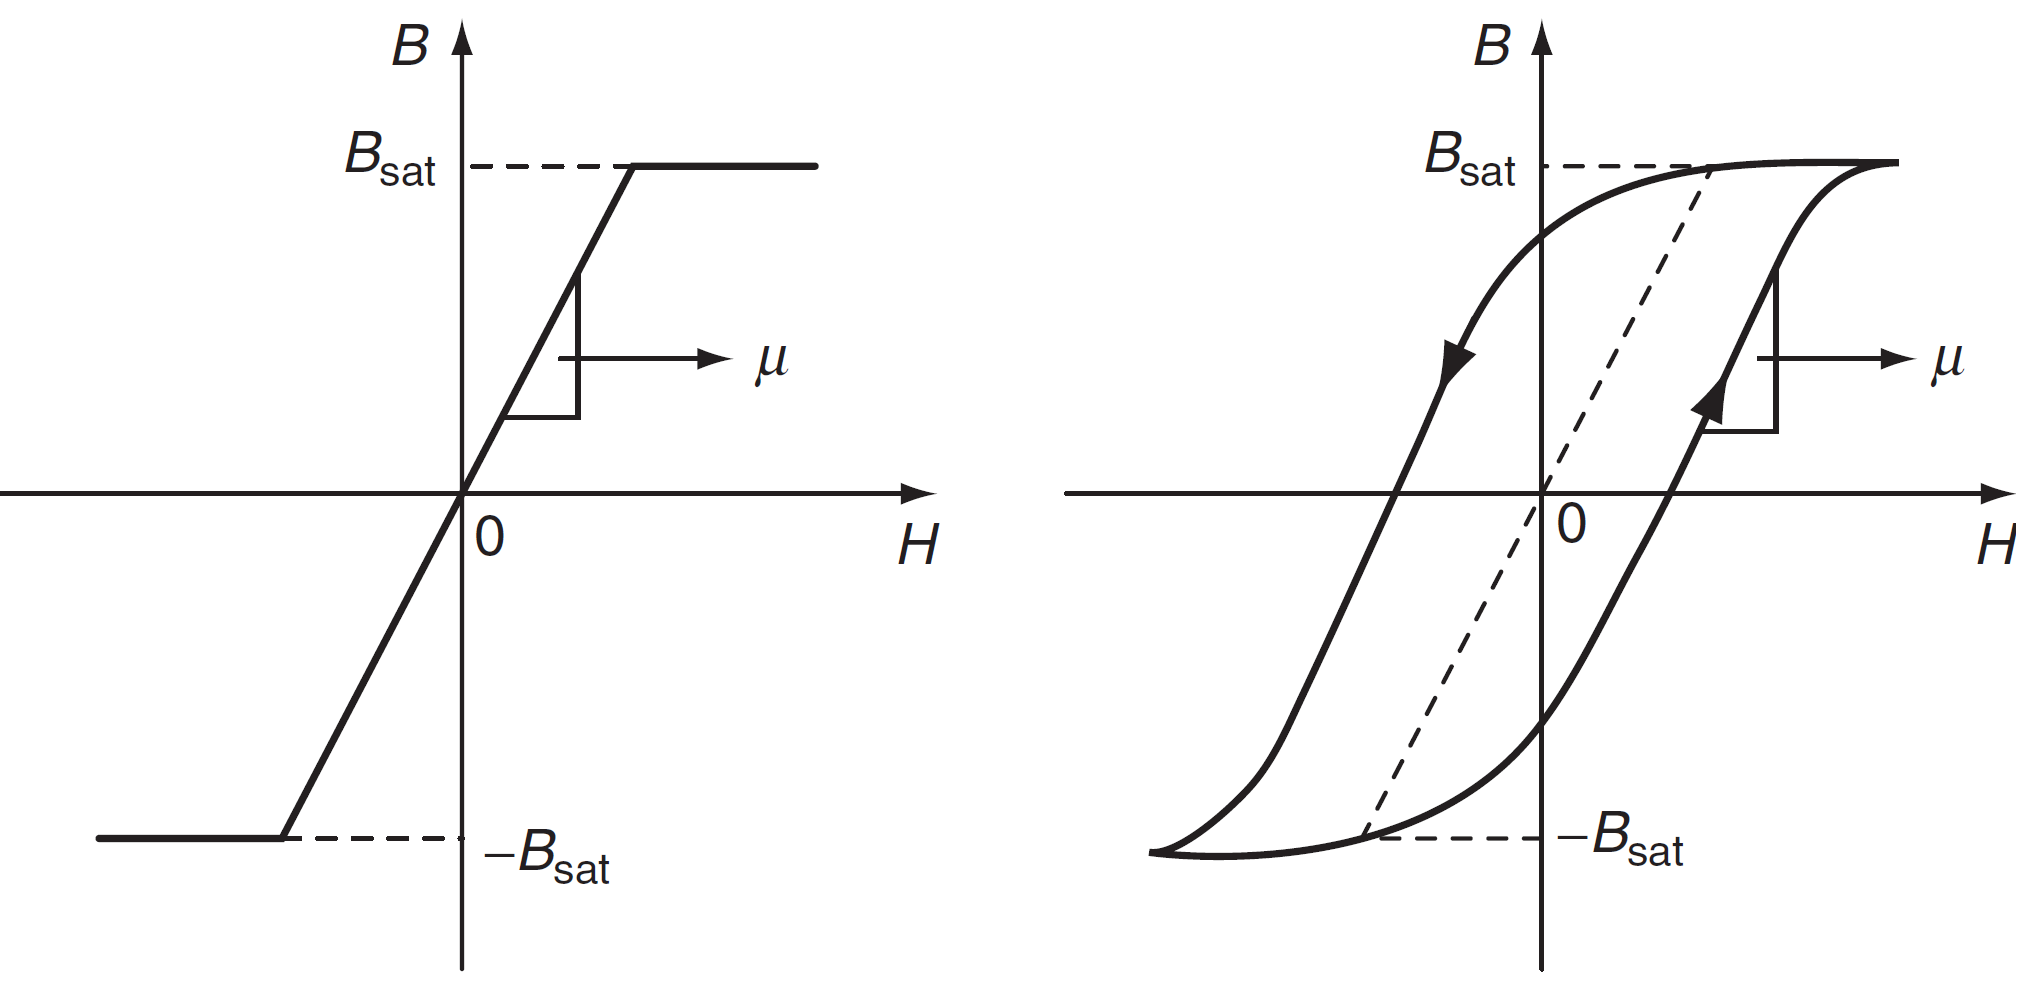
\includegraphics[width=\linewidth]{fig/lec07/BH_loop.png}
                \caption{Piecewise-linear and practical $B$--$H$ characteristics, including hysteresis loop behaviour. Adapted from Umanand, \textit{Power Electronics: Essentials and Applications}}
            \end{figure}
        \end{column}
    \end{columns}
\end{frame}


%%%%%%%%%%%%%%%%%%%%%%%%%%%%%%%%%%%%%%%%%%%%%%%%%%%%%%%%%%%%%
%% Eddy current loss
%%%%%%%%%%%%%%%%%%%%%%%%%%%%%%%%%%%%%%%%%%%%%%%%%%%%%%%%%%%%%
\begin{frame}
    \frametitle{Eddy-Current Loss in the Core}

    \begin{columns}
        \begin{column}{0.58\textwidth}
            A time-varying magnetic flux induces voltage inside conductive magnetic material. This voltage drives circulating currents called eddy currents. Eddy currents cause resistive heating inside the core:
            \begin{align}
                P_{\mathrm{eddy}} \sim i_{\mathrm{eddy}}^2 R_{\mathrm{core}}
            \end{align}
            Eddy-current loss increases strongly with frequency. This is why:
            \begin{itemize}
                \item Laminated steel is used at low line frequency.
                \item Ferrites are preferred at high frequency.
                \item Nanocrystalline and amorphous materials require careful loss evaluation.
            \end{itemize}
            High electrical resistivity of ferrite suppresses core eddy currents.
        \end{column}

        \begin{column}{0.38\textwidth}
            \begin{figure}
                \centering
                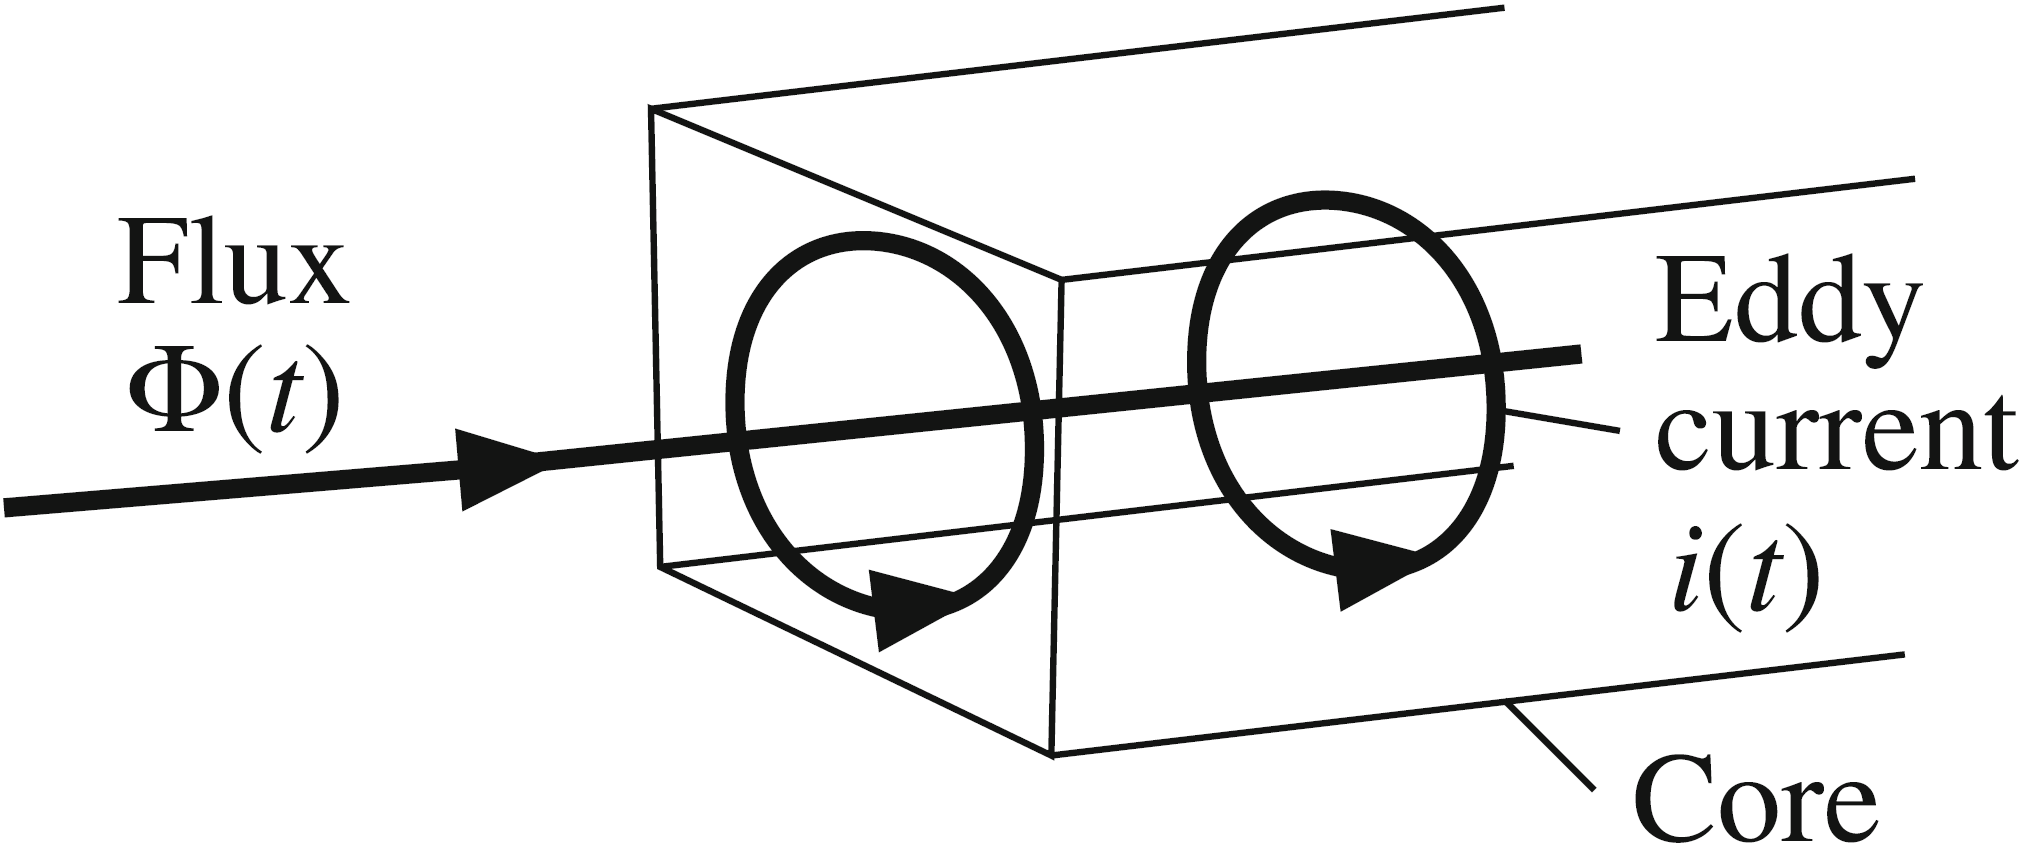
\includegraphics[width=\linewidth]{fig/lec07/eddy_current.png}
                \caption{Eddy currents induced in a magnetic core by time-varying flux. Adapted from Erickson and Maksimovi\'c, \textit{Fundamentals of Power Electronics}, 3rd edition}
            \end{figure}
        \end{column}
    \end{columns}
\end{frame}


%%%%%%%%%%%%%%%%%%%%%%%%%%%%%%%%%%%%%%%%%%%%%%%%%%%%%%%%%%%%%
%% Skin and proximity
%%%%%%%%%%%%%%%%%%%%%%%%%%%%%%%%%%%%%%%%%%%%%%%%%%%%%%%%%%%%%
\begin{frame}
    \frametitle{Skin Effect and Proximity Effect}

    \begin{columns}
        \begin{column}{0.58\textwidth}
            AC winding loss is usually much larger than DC winding loss at high frequency.
            \textbf{Skin effect:}
            \begin{itemize}
                \item Current crowds near the surface of a conductor.
                \item Effective conducting area decreases.
                \item AC resistance increases with frequency.
            \end{itemize}
            \begin{align}
                \delta = \sqrt{\frac{2\rho}{\omega\mu}}
            \end{align}
            \textbf{Proximity effect:}
            \begin{itemize}
                \item Nearby conductors impose additional magnetic fields.
                \item Current distribution becomes non-uniform.
                \item Multilayer windings can suffer severe AC resistance increase.
            \end{itemize}
        \end{column}
        \begin{column}{0.38\textwidth}
            \begin{figure}
                \centering
                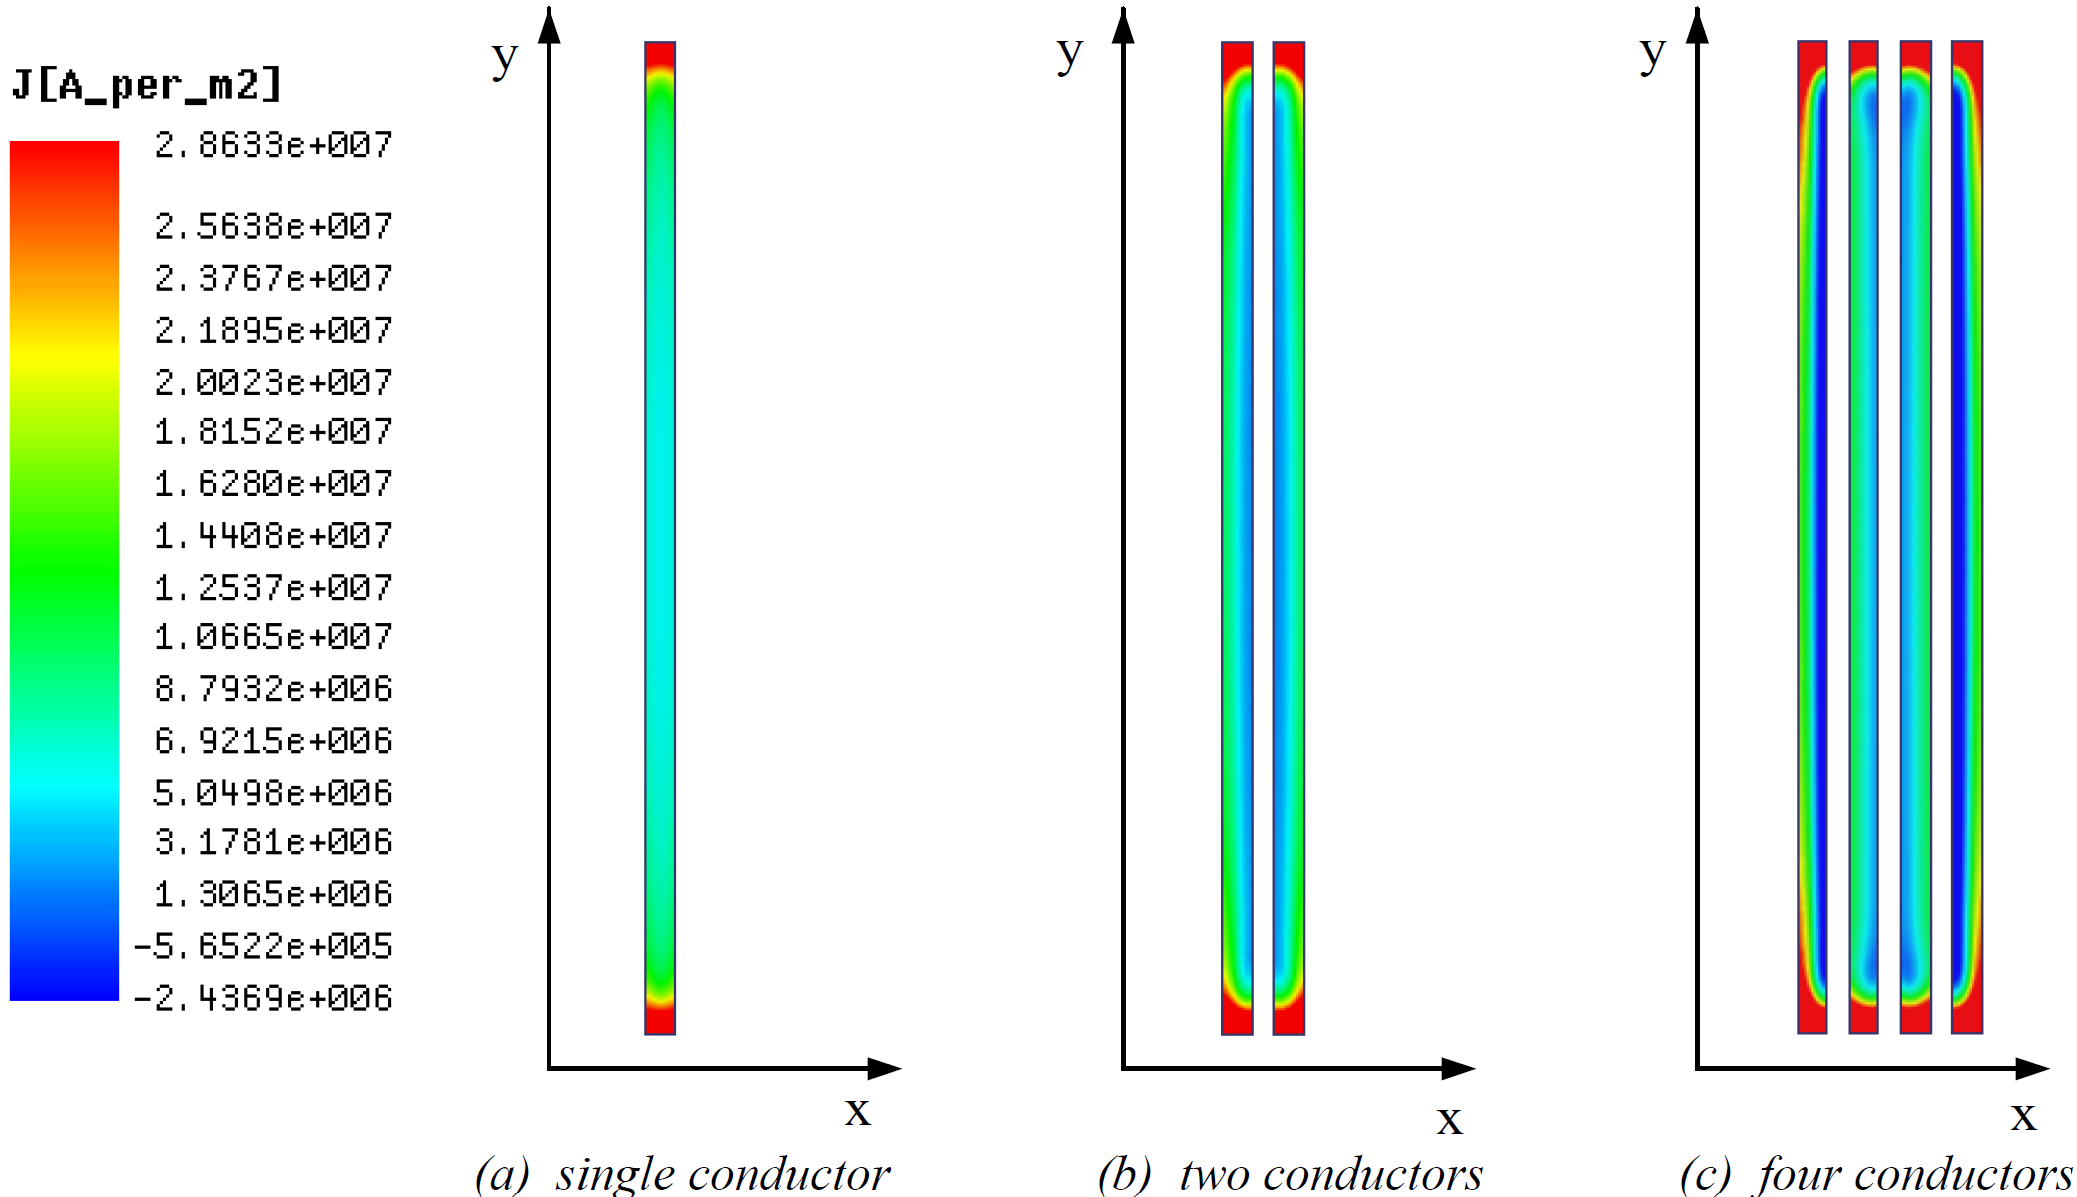
\includegraphics[width=\linewidth]{fig/lec07/current_density_distribution.png}
                \caption{Current-density distribution in single and multiple conductors showing skin and proximity effects. Adapted from Ouyang, \textit{Advances in Planar and Integrated Magnetics}}
            \end{figure}
        \end{column}
    \end{columns}
\end{frame}


%%%%%%%%%%%%%%%%%%%%%%%%%%%%%%%%%%%%%%%%%%%%%%%%%%%%%%%%%%%%%
%% Fringing and gapped inductor loss
%%%%%%%%%%%%%%%%%%%%%%%%%%%%%%%%%%%%%%%%%%%%%%%%%%%%%%%%%%%%%
\begin{frame}
    \frametitle{Fringing-Field Loss in Gapped Inductors}
            In gapped inductors and flyback magnetic components, the air gap stores most of the recoverable magnetic energy.

            \vspace{0.15cm}

            However, the gap also creates fringing flux. This flux can cut nearby windings and induce additional eddy-current loss.

            \vspace{0.15cm}

            Practical consequences:
            \begin{itemize}
                \item Local hot spots near the air gap
                \item Increased AC resistance
                \item Strong dependence on gap location
                \item Need for keep-away regions around the gap
            \end{itemize}

            \vspace{0.15cm}

            Distributed gaps or moving the gap away from windings can reduce fringing-field loss.

\end{frame}

\begin{frame}
    \frametitle{Fringing-Field Loss in Gapped Inductors}
            \begin{figure}
                \centering
                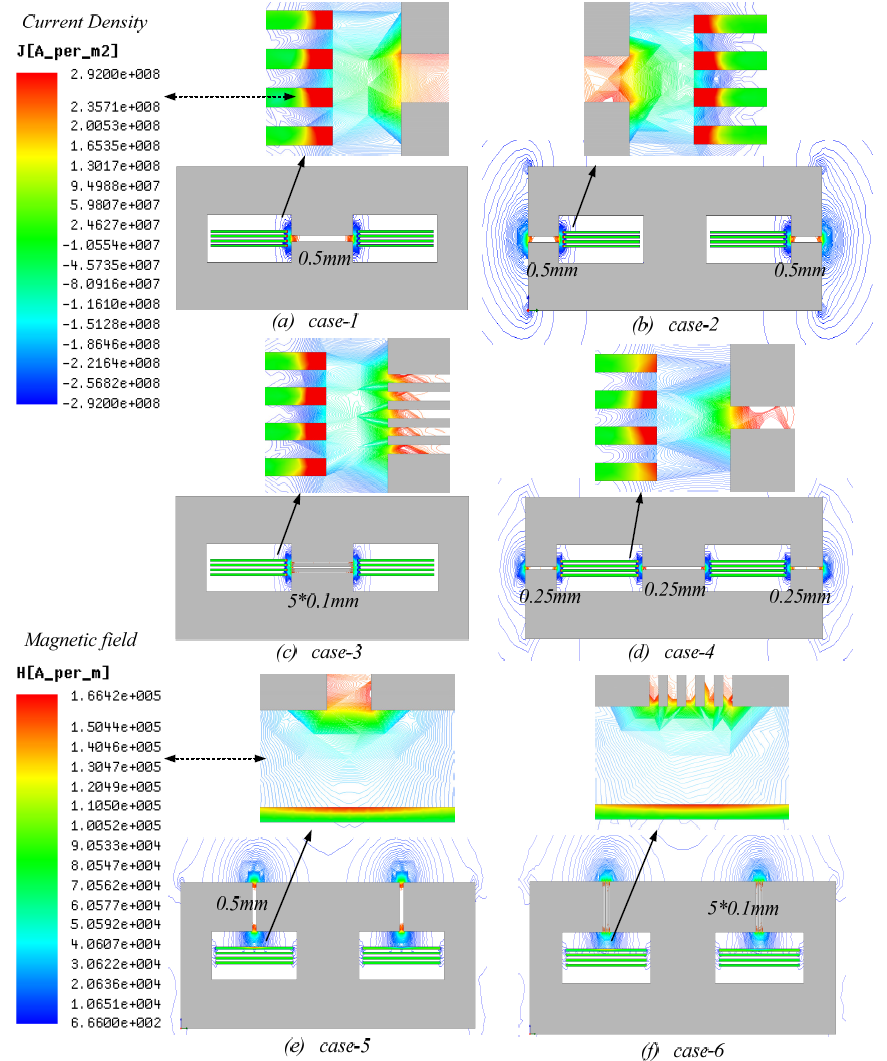
\includegraphics[width=0.3\linewidth]{fig/lec07/fringing_gap_cases.png}
                \caption{Comparison of fringing effects for different air-gap arrangements using 2-D FEA. Adapted from Ouyang, \textit{Advances in Planar and Integrated Magnetics}}
            \end{figure}
\end{frame}
%%%%%%%%%%%%%%%%%%%%%%%%%%%%%%%%%%%%%%%%%%%%%%%%%%%%%%%%%%%%%
%% Copper vs core loss trade-off
%%%%%%%%%%%%%%%%%%%%%%%%%%%%%%%%%%%%%%%%%%%%%%%%%%%%%%%%%%%%%
\begin{frame}
    \frametitle{Copper Loss versus Core Loss Trade-off}

    \begin{columns}
        \begin{column}{0.58\textwidth}
            Magnetic design is an optimization problem, not a single-equation calculation. If the designer increases the flux density:
            \begin{itemize}
                \item Fewer turns are required.
                \item Winding length decreases.
                \item Copper loss may decrease.
                \item Core loss increases.
            \end{itemize}
            If the designer decreases the flux density:
            \begin{itemize}
                \item More turns are required.
                \item Copper loss may increase.
                \item Core loss decreases.
                \item Core may become larger.
            \end{itemize}
        \end{column}

        \begin{column}{0.38\textwidth}
            \begin{align}
                P_{\mathrm{total}} =
                P_{\mathrm{core}} + P_{\mathrm{Cu,dc}} + P_{\mathrm{Cu,ac}}
            \end{align}
            \begin{block}{Design Objective}
                \small
                Do not minimize core loss alone or copper loss alone.

                \vspace{0.15cm}

                Select geometry, turns, flux density, and winding layout to minimize total loss subject to thermal, insulation, and parasitic constraints.
            \end{block}
        \end{column}
    \end{columns}
\end{frame}


%%%%%%%%%%%%%%%%%%%%%%%%%%%%%%%%%%%%%%%%%%%%%%%%%%%%%%%%%%%%%
%% Module 5
%%%%%%%%%%%%%%%%%%%%%%%%%%%%%%%%%%%%%%%%%%%%%%%%%%%%%%%%%%%%%
\begin{frame}
\begin{center}
  \textbf{\Huge{Modern Magnetics}}\\[0.4cm]
  \textbf{\Large{Planar, Integrated, MHz, and Thermally-Aware Designs}}
\end{center}
\end{frame}


%%%%%%%%%%%%%%%%%%%%%%%%%%%%%%%%%%%%%%%%%%%%%%%%%%%%%%%%%%%%%
%% Planar magnetics
%%%%%%%%%%%%%%%%%%%%%%%%%%%%%%%%%%%%%%%%%%%%%%%%%%%%%%%%%%%%%
\begin{frame}
    \frametitle{Planar Magnetics}

    \begin{columns}
        \begin{column}{0.40\textwidth}
            Planar magnetics use flat copper windings and low-profile magnetic cores instead of conventional round-wire windings on bobbins.

            Advantages:
            \begin{itemize}
                \item Low profile
                \item Good repeatability
                \item Improved thermal spreading
                \item Easier interleaving
                \item Controlled parasitics
                \item Suitable for automated manufacturing
            \end{itemize}
        \end{column}

        \begin{column}{0.60\textwidth}
            \begin{figure}
                \centering
                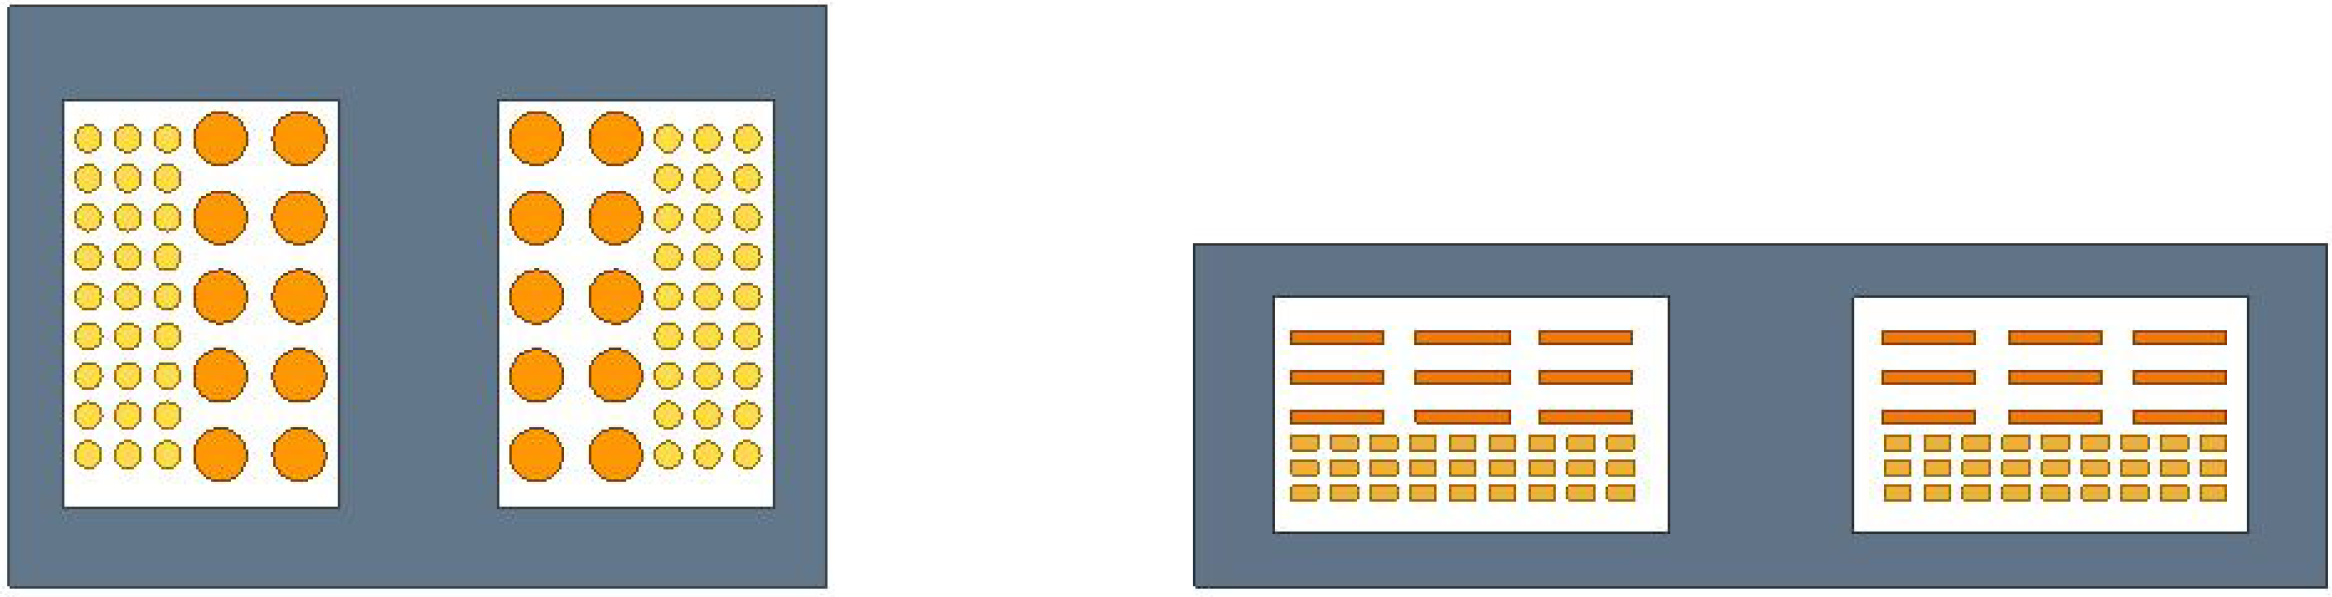
\includegraphics[width=\linewidth]{fig/lec07/standard_vs_planar_cross_section.png}
                \caption{Comparison of standard transformer and planar transformer cross-section structures. Adapted from STMicroelectronics, \textit{How Planar Magnetics Improve Performance in Power Electronics}}
            \end{figure}
        \end{column}
    \end{columns}
\end{frame}


%%%%%%%%%%%%%%%%%%%%%%%%%%%%%%%%%%%%%%%%%%%%%%%%%%%%%%%%%%%%%
%% Planar magnetics
%%%%%%%%%%%%%%%%%%%%%%%%%%%%%%%%%%%%%%%%%%%%%%%%%%%%%%%%%%%%%
\begin{frame}
    \frametitle{Planar Magnetics}
    \begin{columns}
        \begin{column}{0.38\textwidth}
            Drawbacks:
            \begin{itemize}
                \item Larger footprint
                \item Lower copper fill factor
                \item Limited number of turns
                \item Higher interwinding capacitance
                \item PCB manufacturing constraints
            \end{itemize}
        \end{column}

        \begin{column}{0.60\textwidth}
            \begin{figure}
                \centering
                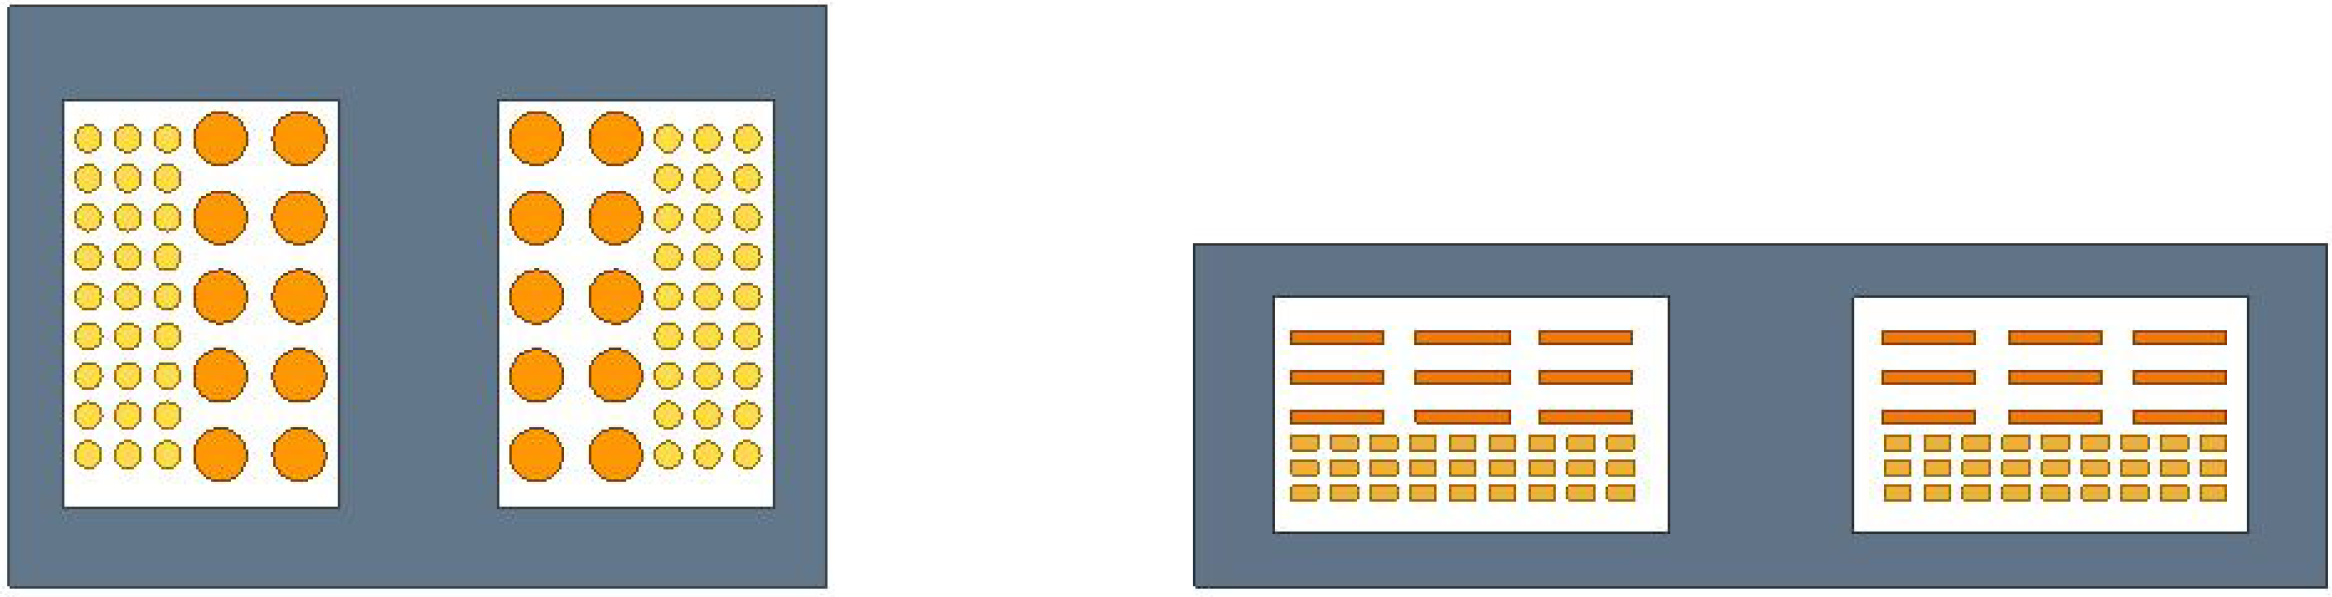
\includegraphics[width=\linewidth]{fig/lec07/standard_vs_planar_cross_section.png}
                \caption{Comparison of standard transformer and planar transformer cross-section structures. Adapted from STMicroelectronics, \textit{How Planar Magnetics Improve Performance in Power Electronics}}
            \end{figure}
        \end{column}
    \end{columns}
\end{frame}


%%%%%%%%%%%%%%%%%%%%%%%%%%%%%%%%%%%%%%%%%%%%%%%%%%%%%%%%%%%%%
%% Planar construction
%%%%%%%%%%%%%%%%%%%%%%%%%%%%%%%%%%%%%%%%%%%%%%%%%%%%%%%%%%%%%
\begin{frame}
    \frametitle{Planar Transformer Construction}

    \begin{columns}
        \begin{column}{0.58\textwidth}
            A planar transformer is usually built from:
            \begin{itemize}
                \item Low-profile ferrite core
                \item PCB or flexible-PCB winding layers
                \item Copper traces or stamped copper turns
                \item Insulation layers
                \item Vias or pins for interconnection
            \end{itemize}

            The geometry fixes the winding positions very precisely. Therefore, leakage inductance, capacitance, and resistance are more repeatable than in manually wound transformers.

            \vspace{0.15cm}

            This is a major advantage in resonant converters, where leakage inductance and parasitic capacitance can strongly affect the gain and EMI behaviour.
        \end{column}

        \begin{column}{0.38\textwidth}
            \begin{figure}
                \centering
                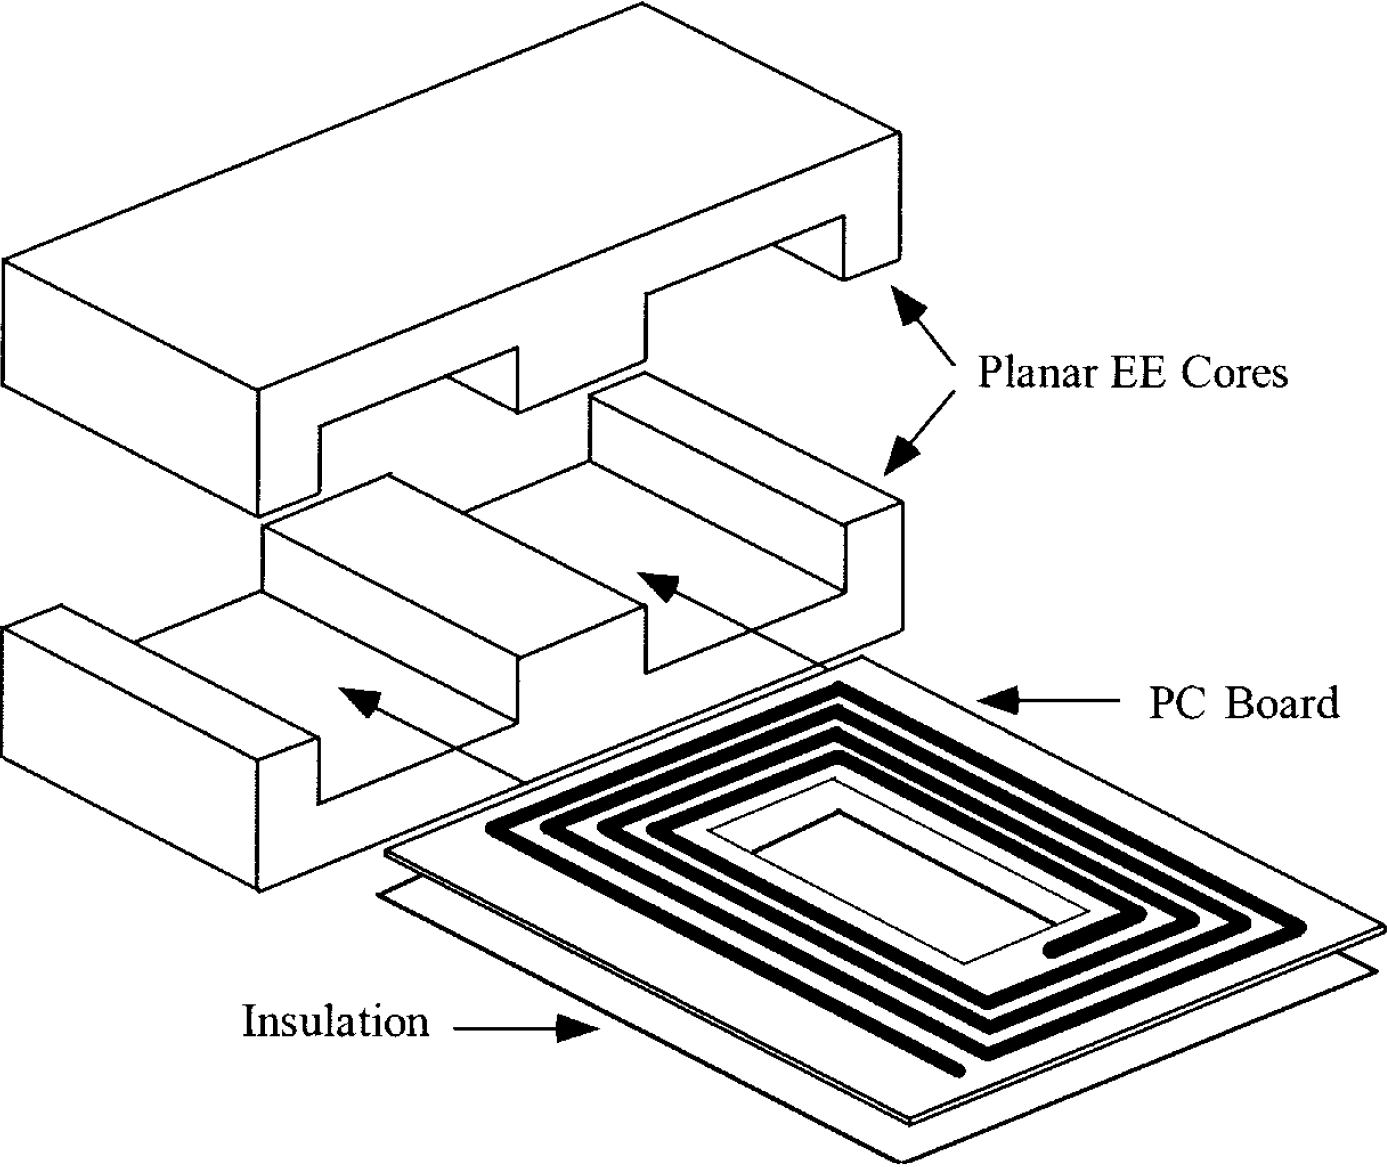
\includegraphics[width=\linewidth]{fig/lec07/planar_EE_perspective.png}
                \caption{Perspective view of a typical EE planar transformer using PC-board windings and planar EE cores. Adapted from \textit{Transformer and Inductor Design Handbook}}
            \end{figure}
        \end{column}
    \end{columns}
\end{frame}


%%%%%%%%%%%%%%%%%%%%%%%%%%%%%%%%%%%%%%%%%%%%%%%%%%%%%%%%%%%%%
%% PCB integrated transformer
%%%%%%%%%%%%%%%%%%%%%%%%%%%%%%%%%%%%%%%%%%%%%%%%%%%%%%%%%%%%%
\begin{frame}
    \frametitle{PCB-Integrated Planar Transformer}

    \begin{columns}
        \begin{column}{0.58\textwidth}
            Planar magnetics can be integrated into the main converter PCB. This reduces separate component count and improves mechanical repeatability.

            \vspace{0.15cm}

            A PCB-integrated transformer typically uses:
            \begin{itemize}
                \item Multiple copper layers for primary and secondary turns
                \item Vias for layer-to-layer connections
                \item Ferrite core halves inserted around the PCB
                \item Controlled insulation layers between primary and secondary
            \end{itemize}
        \end{column}

        \begin{column}{0.38\textwidth}
            \begin{figure}
                \centering
                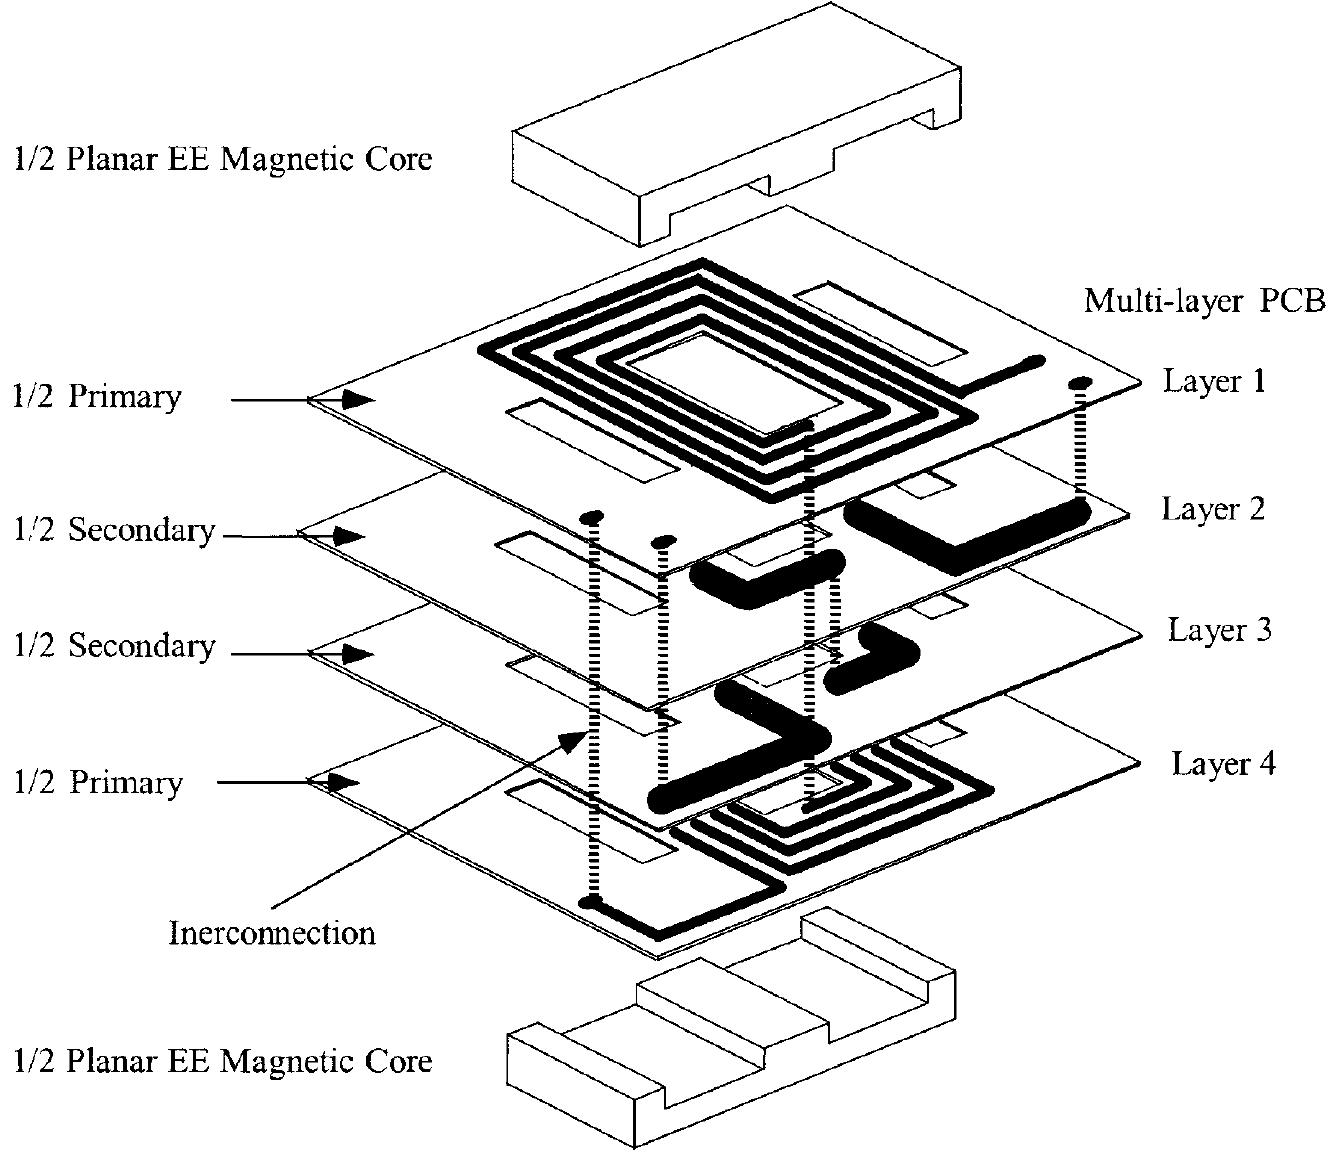
\includegraphics[width=\linewidth]{fig/lec07/planer_trans.png}
                \caption{Planar transformer integrated into the main PC board and final assembly. Adapted from \textit{Transformer and Inductor Design Handbook}, Chapter 20, Figs. 20-5 and 20-6.}
            \end{figure}
        \end{column}
    \end{columns}
\end{frame}



%%%%%%%%%%%%%%%%%%%%%%%%%%%%%%%%%%%%%%%%%%%%%%%%%%%%%%%%%%%%%
%% PCB integrated transformer
%%%%%%%%%%%%%%%%%%%%%%%%%%%%%%%%%%%%%%%%%%%%%%%%%%%%%%%%%%%%%
\begin{frame}
    \frametitle{PCB-Integrated Planar Transformer}

    \begin{columns}
        \begin{column}{0.58\textwidth}
            The design challenge is to simultaneously satisfy:
            \begin{itemize}
                \item Copper loss limit
                \item Core loss limit
                \item Isolation requirement
                \item Leakage and capacitance targets
                \item PCB manufacturing rules
            \end{itemize}
        \end{column}

        \begin{column}{0.38\textwidth}
            \begin{figure}
                \centering
                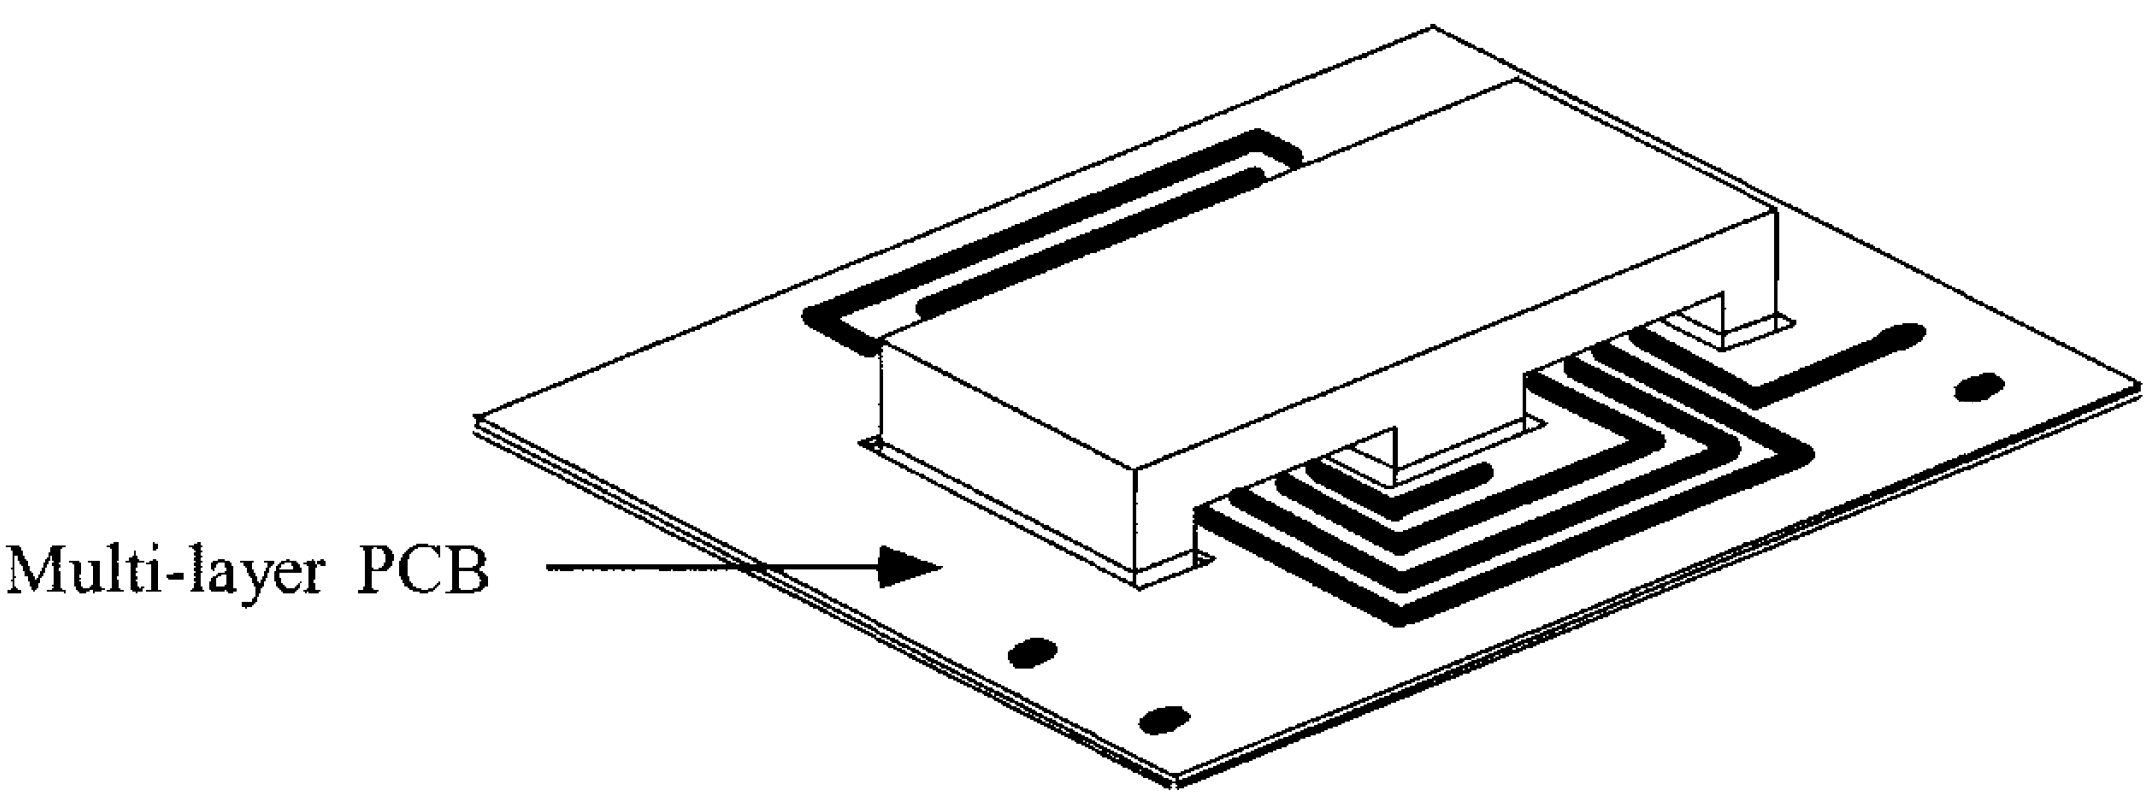
\includegraphics[width=\linewidth]{fig/lec07/planar_trans_assembly.png}
                \caption{Planar transformer integrated into the main PC board and final assembly. Adapted from \textit{Transformer and Inductor Design Handbook}, Chapter 20, Figs. 20-5 and 20-6.}
            \end{figure}
        \end{column}
    \end{columns}
\end{frame}


%%%%%%%%%%%%%%%%%%%%%%%%%%%%%%%%%%%%%%%%%%%%%%%%%%%%%%%%%%%%%
%% Modeling planar magnetics
%%%%%%%%%%%%%%%%%%%%%%%%%%%%%%%%%%%%%%%%%%%%%%%%%%%%%%%%%%%%%
\begin{frame}
    \frametitle{Modeling Planar Magnetics}

    \begin{columns}
        \begin{column}{0.58\textwidth}
            Planar magnetics are attractive, but they require accurate modeling because skin effect, proximity effect, vias, gaps, and layer coupling strongly influence performance.

            The Modular Layer Model represents each PCB layer as an impedance network. This allows the designer to predict:
            \begin{itemize}
                \item Current sharing
                \item AC resistance
                \item Winding impedance
                \item Stored reactive energy
                \item Field distribution
                \item Loss distribution
            \end{itemize}

            \vspace{0.15cm}
        \end{column}

        \begin{column}{0.38\textwidth}
            \begin{figure}
                \centering
                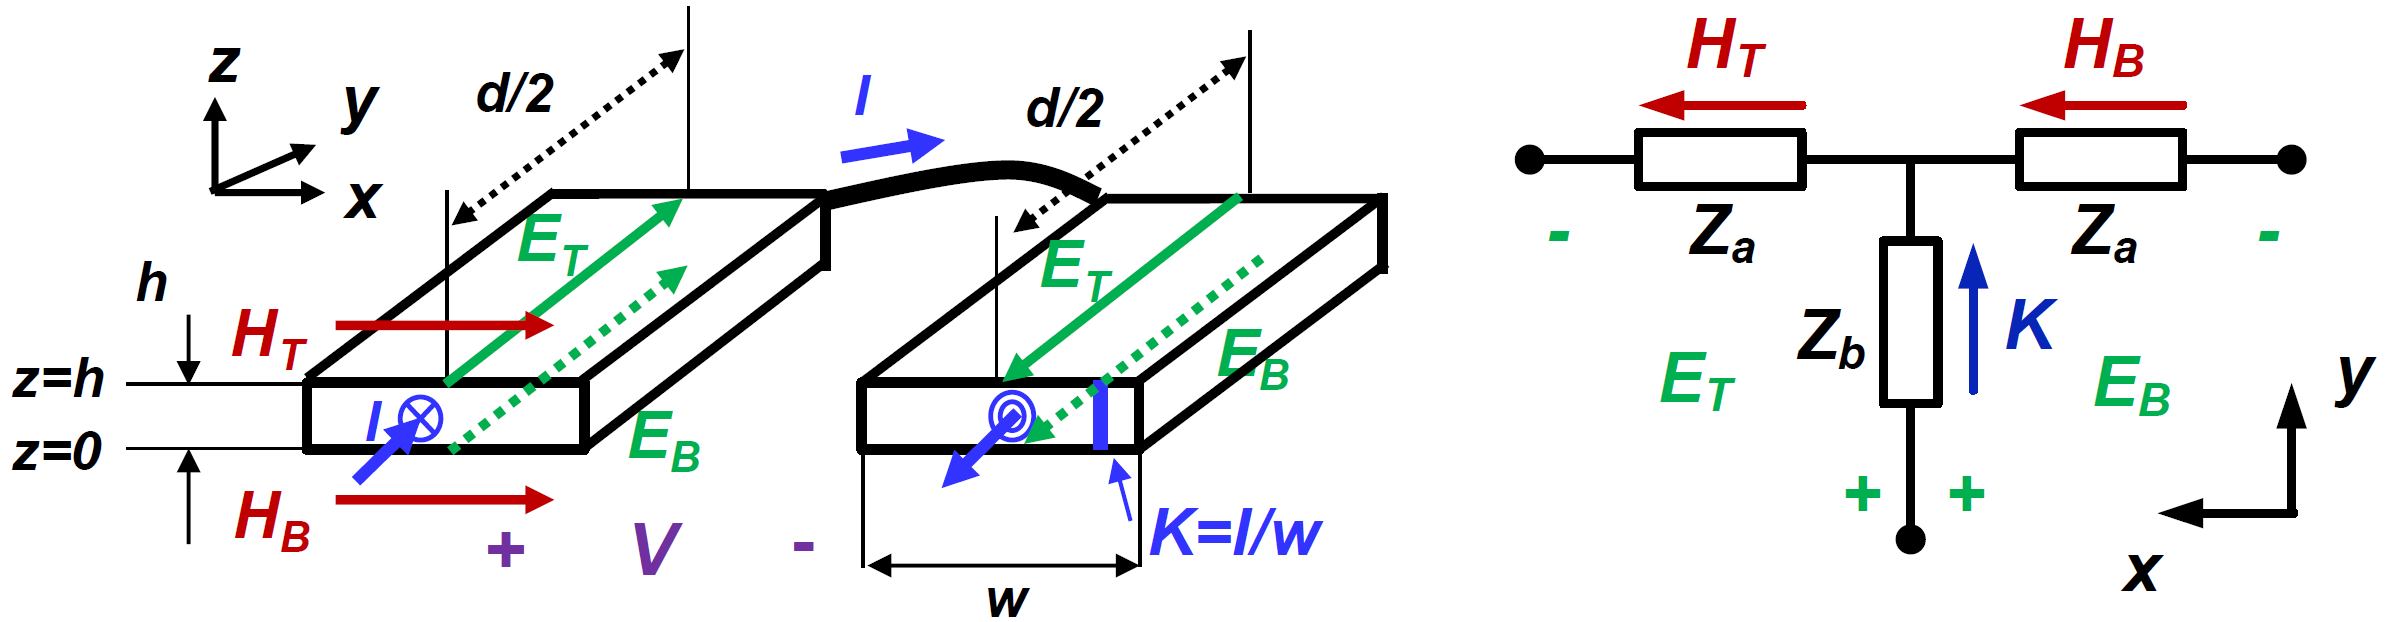
\includegraphics[width=\linewidth]{fig/lec07/one_turn_layer_model.png}
                \caption{One-turn planar layer and its three-terminal impedance network. Adapted from Chen et al., \textit{A Systematic Approach to Modeling Impedances and Current Distribution in Planar Magnetics}}
            \end{figure}
        \end{column}
    \end{columns}
Such models are useful before moving to detailed 2-D or 3-D finite-element simulations.
\end{frame}


%%%%%%%%%%%%%%%%%%%%%%%%%%%%%%%%%%%%%%%%%%%%%%%%%%%%%%%%%%%%%
%% MHz magnetics
%%%%%%%%%%%%%%%%%%%%%%%%%%%%%%%%%%%%%%%%%%%%%%%%%%%%%%%%%%%%%
\begin{frame}
    \frametitle{MHz Magnetics}

    \begin{columns}
        \begin{column}{0.58\textwidth}
            Wide-bandgap devices enable switching frequencies from hundreds of kHz into the MHz range.

            Higher frequency can reduce magnetic size because volt-seconds per cycle decrease:
            \begin{align}
                \Delta B =
                \frac{1}{N A_c}\int v(t)\,dt
            \end{align}
            However, MHz magnetics face severe constraints:
            \begin{itemize}
                \item Core loss rises rapidly with frequency
                \item AC winding resistance increases
                \item Parasitic capacitance becomes circuit-relevant
                \item Thermal paths become critical
                \item Layout and EMI dominate behaviour
            \end{itemize}
        \end{column}
        \begin{column}{0.38\textwidth}
            Ferrites, air-core structures, PCB windings, and thin low-loss cores are often considered.
            \begin{block}{MHz Design Message}
                \small
                Increasing frequency reduces magnetic volume only if core loss, winding loss, thermal rise, and EMI remain controlled.
            \end{block}
        \end{column}
    \end{columns}
\end{frame}


%%%%%%%%%%%%%%%%%%%%%%%%%%%%%%%%%%%%%%%%%%%%%%%%%%%%%%%%%%%%%
%% Integrated magnetics
%%%%%%%%%%%%%%%%%%%%%%%%%%%%%%%%%%%%%%%%%%%%%%%%%%%%%%%%%%%%%
\begin{frame}
    \frametitle{Integrated Magnetics}
            Integrated magnetics combine multiple magnetic functions into one magnetic structure.

            Examples include:
            \begin{itemize}
                \item Transformer plus resonant inductor
                \item Transformer plus output filter inductor
                \item Coupled inductors for multiphase converters
                \item Current balancing transformer plus common inductor
            \end{itemize}

            \vspace{0.15cm}

            Potential benefits:
            \begin{itemize}
                \item Fewer magnetic components
                \item Reduced converter volume
                \item Better power density
                \item Controlled leakage or coupling
                \item Lower assembly cost
            \end{itemize}

            The main challenge is controlling flux paths so that the intended functions are coupled while unwanted interactions are avoided.
\end{frame}


%%%%%%%%%%%%%%%%%%%%%%%%%%%%%%%%%%%%%%%%%%%%%%%%%%%%%%%%%%%%%
%% Cooling
%%%%%%%%%%%%%%%%%%%%%%%%%%%%%%%%%%%%%%%%%%%%%%%%%%%%%%%%%%%%%
\begin{frame}
    \frametitle{Cooling and Thermal Paths in Magnetics}
    \begin{columns}
        \begin{column}{0.58\textwidth}
            Magnetic components must be designed thermally as well as electrically.

            Heat sources:
            \begin{itemize}
                \item Core loss
                \item DC copper loss
                \item AC winding loss
                \item Fringing-induced local loss
                \item Termination and via loss
            \end{itemize}
        \end{column}

        \begin{column}{0.38\textwidth}
            \begin{figure}
                \centering
                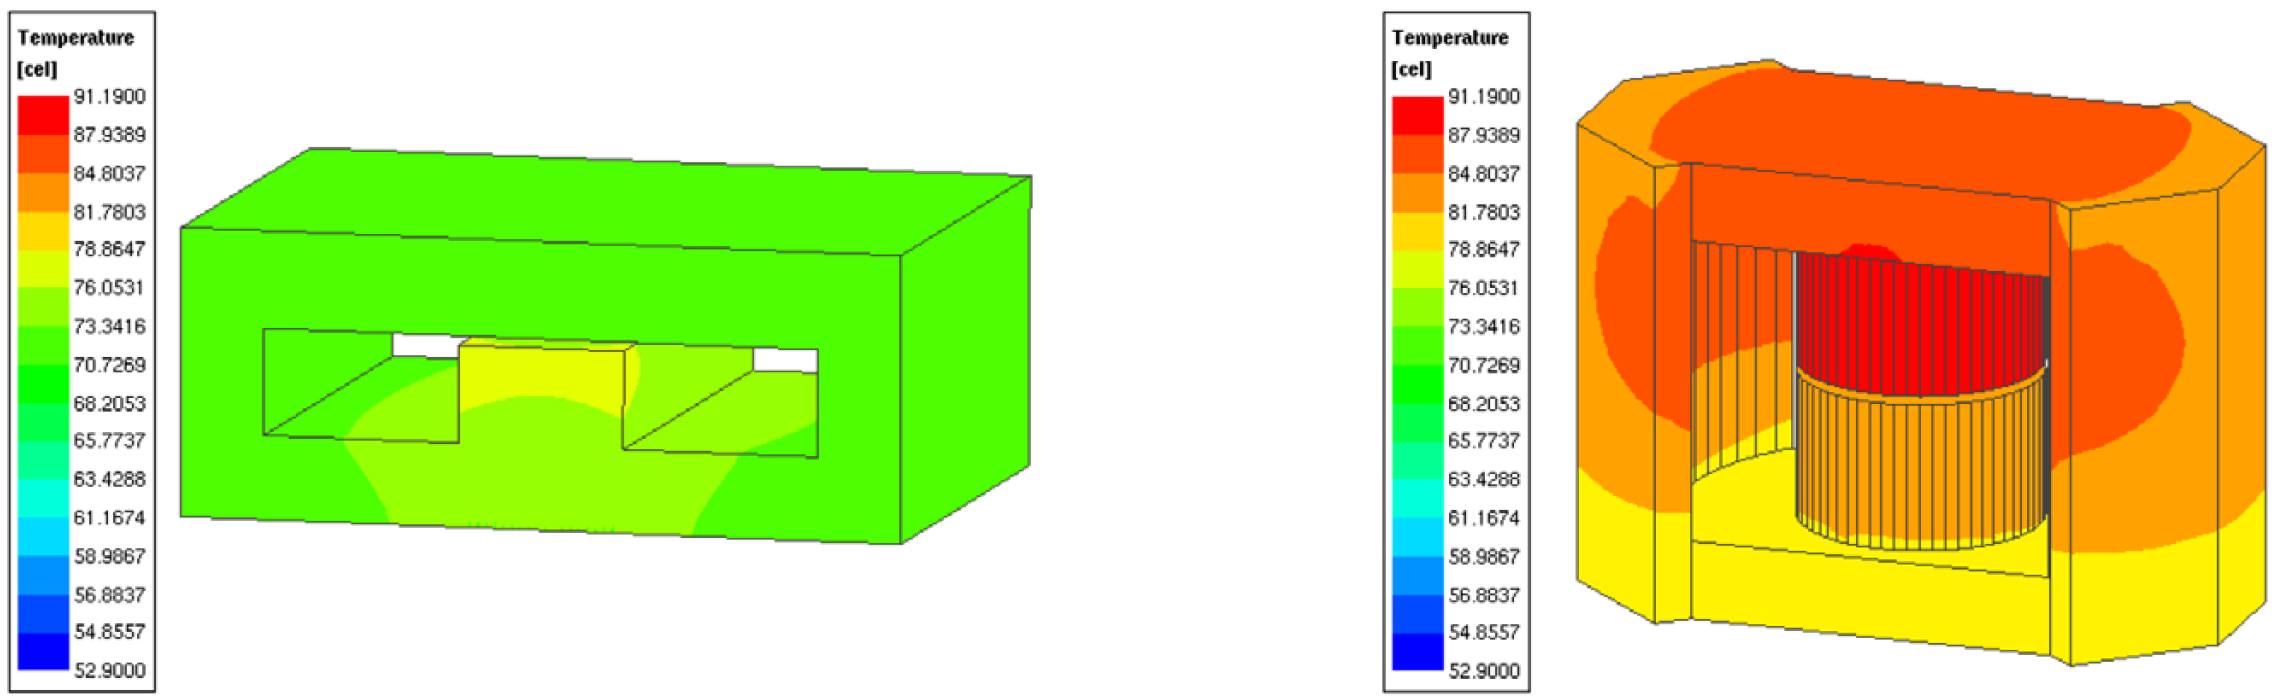
\includegraphics[width=\linewidth]{fig/lec07/thermal_profiles.png}
                \caption{Thermal comparison of planar and concentric transformers, including the effect of an aluminum dissipation plane. Adapted from STMicroelectronics, \textit{How Planar Magnetics Improve Performance in Power Electronics}, Figs. 4 and 5.}
            \end{figure}
        \end{column}
    \end{columns}
\end{frame}


%%%%%%%%%%%%%%%%%%%%%%%%%%%%%%%%%%%%%%%%%%%%%%%%%%%%%%%%%%%%%
%% Cooling
%%%%%%%%%%%%%%%%%%%%%%%%%%%%%%%%%%%%%%%%%%%%%%%%%%%%%%%%%%%%%
\begin{frame}
    \frametitle{Cooling and Thermal Paths in Magnetics}
    \begin{columns}
        \begin{column}{0.58\textwidth}
            Cooling options:
            \begin{itemize}
                \item Natural convection
                \item Forced-air cooling
                \item Heat spreading through PCB copper
                \item Aluminum baseplate or heat spreader
                \item Liquid-cooled cold plate for high power density
            \end{itemize}
            Planar cores often have favourable surface-to-volume ratio, improving heat spreading.
        \end{column}

        \begin{column}{0.38\textwidth}
            \begin{figure}
                \centering
                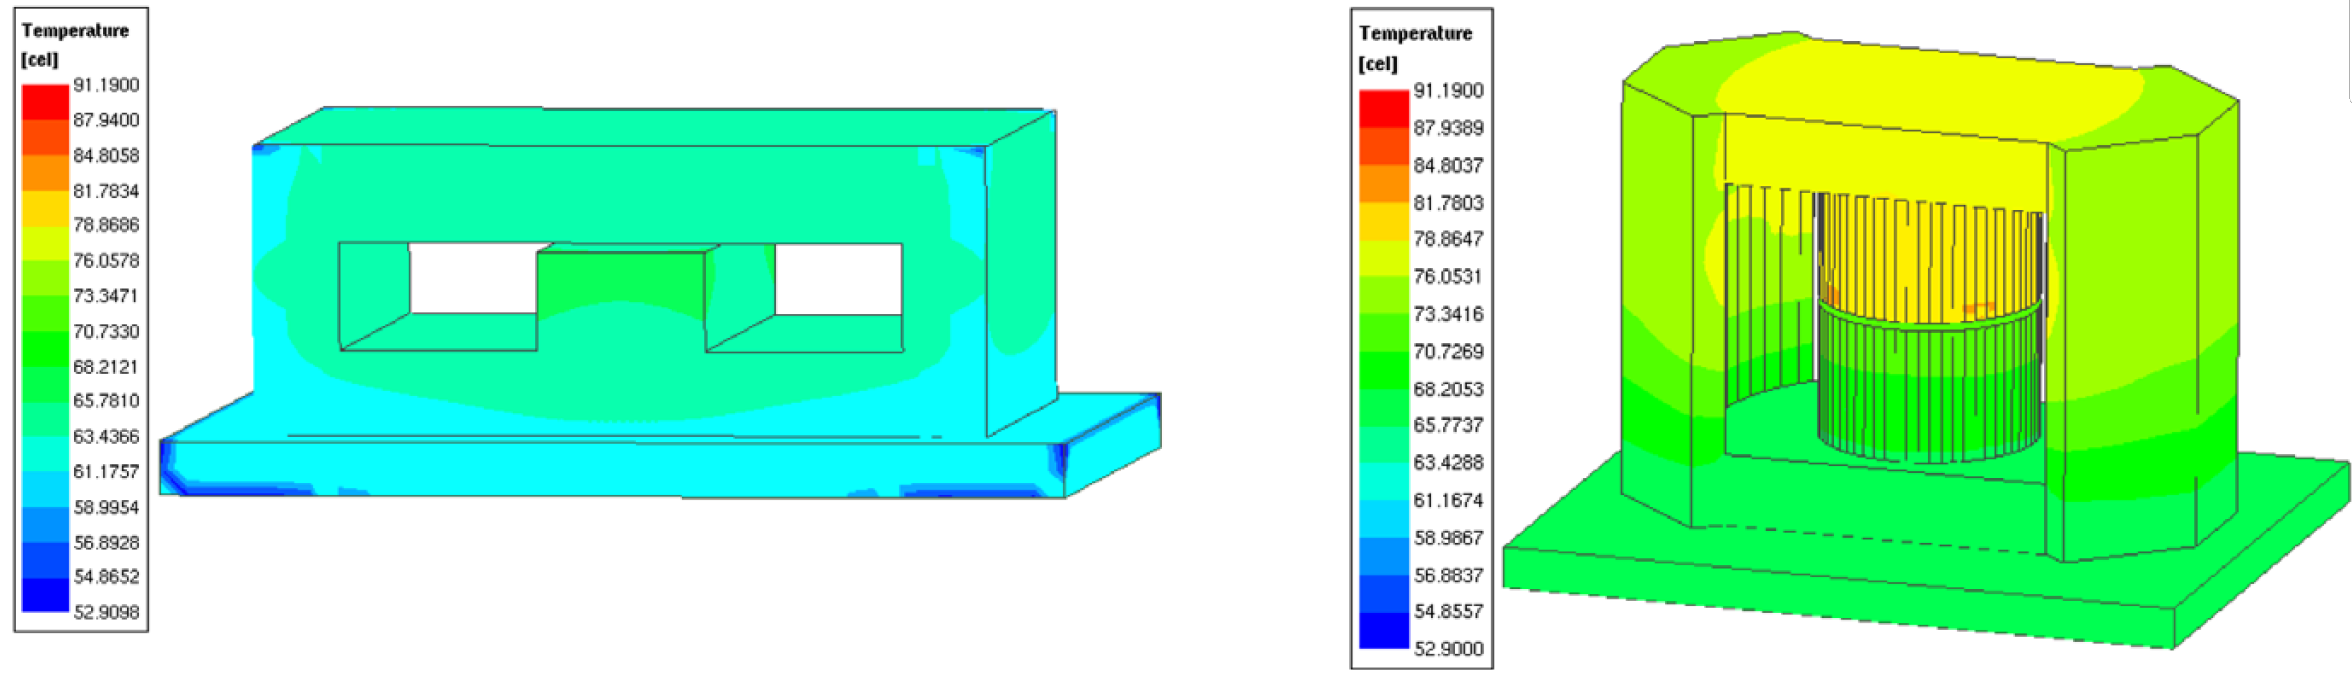
\includegraphics[width=\linewidth]{fig/lec07/thermal_profiles_2.png}
                \caption{Thermal comparison of planar and concentric transformers, including the effect of an aluminum dissipation plane. Adapted from STMicroelectronics, \textit{How Planar Magnetics Improve Performance in Power Electronics}, Figs. 4 and 5.}
            \end{figure}
        \end{column}
    \end{columns}
\end{frame}

%%%%%%%%%%%%%%%%%%%%%%%%%%%%%%%%%%%%%%%%%%%%%%%%%%%%%%%%%%%%%
%% Conventional to future magnetics
%%%%%%%%%%%%%%%%%%%%%%%%%%%%%%%%%%%%%%%%%%%%%%%%%%%%%%%%%%%%%
\begin{frame}
    \frametitle{Evolution of Magnetic Components}

    \scriptsize
    \begin{table}
        \centering
        \begin{tabular}{p{0.18\textwidth}p{0.23\textwidth}p{0.26\textwidth}p{0.22\textwidth}}
            \hline
            \textbf{Technology} & \textbf{Main Feature} & \textbf{Strength} & \textbf{Challenge}\\
            \hline
            Conventional wire-wound & Round wire on bobbin & Mature, flexible, low cost & Large size and variable parasitics\\
            Foil / Litz magnetics & Optimized conductor geometry & Lower AC loss & Manufacturing and termination complexity\\
            Planar magnetics & PCB or flat copper winding & Low profile, repeatable, good thermal spreading & Low fill factor and capacitance\\
            Integrated magnetics & Multiple magnetic functions in one core & Higher power density & Complex flux-path design\\
            Future 3-D / additive magnetics & Geometrically optimized cores and windings & Custom field shaping & Material, cost, and qualification issues\\
            \hline
        \end{tabular}
    \end{table}

    \vspace{0.15cm}

    \begin{block}{Conclusion}
        \small
        Modern magnetic design is moving from component selection toward co-design of core, winding, layout, thermal path, converter topology, and switching frequency.
    \end{block}
\end{frame}


%%%%%%%%%%%%%%%%%%%%%%%%%%%%%%%%%%%%%%%%%%%%%%%%%%%%%%%%%%%%%
%% Final magnetics summary
%%%%%%%%%%%%%%%%%%%%%%%%%%%%%%%%%%%%%%%%%%%%%%%%%%%%%%%%%%%%%
\begin{frame}
    \frametitle{Concluding Remarks on Magnetics}

    \begin{itemize}
        \item Magnetic components are not auxiliary parts; they often define the achievable efficiency, size, EMI performance, and thermal limit of a converter.

        \item Inductors, transformers, coupled inductors, flyback magnetics, and current transformers have different design objectives.

        \item Transformer design begins from volt-seconds, turns ratio, current waveforms, isolation, and thermal constraints.

        \item Winding arrangement controls leakage inductance, proximity effect, capacitance, and cooling.

        \item At high frequency, losses are dominated by core loss, skin effect, proximity effect, fringing fields, and parasitics.

        \item Planar and integrated magnetics are powerful technologies for high-power-density converters, but they require careful electromagnetic, thermal, and manufacturing co-design.

        \item For GaN and SiC converters, the magnetic component is often the bottleneck that determines whether MHz operation is practically useful.
    \end{itemize}
\end{frame}

